\documentclass[12pt,oneside,openany]{book}

\usepackage[utf8]{inputenc}
\usepackage[T1]{fontenc}
\usepackage[english]{babel}
\usepackage[a4paper,margin=1in]{geometry}
\usepackage{setspace}
\usepackage{amsmath,amssymb,amsfonts}
\usepackage{graphicx}
\usepackage{booktabs}
\usepackage{array}
\usepackage{longtable}
\usepackage{float}
\usepackage{subcaption}
\usepackage{enumitem}
\usepackage[hidelinks]{hyperref}

\setstretch{1.5}

\renewcommand{\bibname}{References}

\newcommand{\ThesisTitleText}{Target-Driven Memory-Attention-Enhanced Humanoid Parkour}
\newcommand{\ThesisAuthorText}{Your Name}
\newcommand{\ThesisProgramText}{[Name of Program]}
\newcommand{\ThesisThrustText}{[Full Name of Your Thrust]}
\newcommand{\ThesisCompletionDateText}{[Month Year]}
\newcommand{\ThesisAbstractText}{[Abstract text, 300 words or less]}
\newcommand{\SupervisorName}{[Supervisor Name]}
\newcommand{\CoSupervisorName}{[Co-Supervisor Name]}
\newcommand{\ThrustHeadName}{[Thrust Head Name]}

\begin{document}

\frontmatter

\clearpage
\thispagestyle{plain}
\vspace*{25mm}
\begin{center}
{\Large\bfseries \ThesisTitleText\par}
\vspace{5\baselineskip}
by\par
\vspace{1\baselineskip}
{\Large \ThesisAuthorText\par}
\vspace{5\baselineskip}
A Thesis Submitted to\par
The Hong Kong University of Science and Technology (Guangzhou)\par
in Partial Fulfillment of the Requirements for\par
the Degree of Master of Philosophy\par
\ThesisThrustText\par
in \ThesisProgramText\par
\vfill
\ThesisCompletionDateText, Guangzhou\par
\end{center}

\clearpage
\thispagestyle{plain}
\vspace*{25mm}
\begin{center}
{\Large\bfseries \ThesisTitleText\par}
\vspace{1em}
by \ThesisAuthorText\par
\vspace{1em}
\ThesisThrustText\par
The Hong Kong University of Science and Technology (Guangzhou)\par
\vspace{2em}
Abstract\par
\vspace{1em}
\ThesisAbstractText\par
\end{center}

\clearpage
\thispagestyle{plain}
\vspace*{25mm}
Authorization\par
\vspace{1em}
I hereby declare that I am the sole author of the thesis.\par
I authorize the Hong Kong University of Science and Technology (Guangzhou) to lend this thesis to other institutions or individuals for the purpose of scholarly research.\par
I further authorize the Hong Kong University of Science and Technology (Guangzhou) to reproduce the thesis by photocopying or by other means, in total or in part, at the request of other institutions or individuals for the purpose of scholarly research.\par
\vfill
\noindent \ThesisAuthorText\par
\vspace{2\baselineskip}
[Date]\par

\clearpage
\thispagestyle{plain}
\vspace*{25mm}
\begin{center}
{\Large\bfseries \ThesisTitleText\par}
\vspace{1em}
by\par
\vspace{1\baselineskip}
{\Large \ThesisAuthorText\par}
\end{center}
\vspace{2em}
This is to certify that I have examined the above MPhil thesis and have found that it is complete and satisfactory in all respects, and that any and all revisions required by the thesis examination committee have been made.\par
\vspace{3em}
\noindent \SupervisorName, Thesis Supervisor\par
\vspace{1.5em}
\noindent \CoSupervisorName, Thesis Co-Supervisor\par
\vspace{1.5em}
\noindent \ThrustHeadName, Head of Thrust\par
\vfill
\noindent [Date]\par

\tableofcontents
\listoffigures
\listoftables

\mainmatter

\chapter{Introduction and Motivation}

With the continued development of embodied intelligence and humanoid robotics, research has gradually moved from locomotion in structured environments toward operation in complex, dynamic, and uncertain settings. Among the many challenging benchmarks in this direction, humanoid parkour stands out as a representative task because it requires the robot to step over obstacles, climb stairs, traverse gaps, absorb impacts, and recover balance in rapid succession. Compared with standard flat-ground walking, parkour places much stronger demands on perception, planning, control, and whole-body coordination. A robot must not only remain stable, but also maintain motion continuity under changing terrain and respond in real time to disturbances. For this reason, humanoid parkour has become an important testbed for evaluating the agility, robustness, and environmental adaptability of humanoid robots.

From the perspective of control, humanoid parkour is not a single locomotion problem, but a long-horizon decision-making problem that couples sensing, temporal reasoning, and motion generation. During traversal, the robot must continuously interpret partial terrain information, assess the feasibility of upcoming actions, and adjust posture and contact strategy accordingly. The state at one moment influences the range of feasible states in the future, which means that successful control requires an explicit understanding of temporal dependencies rather than only instantaneous observations. In real-world environments, however, observations are often incomplete, noisy, and time-varying. Terrain geometry may change, targets may shift, and unexpected disturbances may occur. These factors make it difficult for conventional methods based on fixed trajectories, short-term optimization, or manually designed rules to achieve reliable performance in complex parkour scenarios.

The difficulty is further amplified in non-structured environments with uncertain friction, irregular footholds, dynamic obstacles, and imperfect model parameters. Under such conditions, the robot must do more than remain upright: it must jump accurately, land safely, transition smoothly between motion primitives, and maintain task progress toward a desired goal. This requires a policy that can identify which historical information is still relevant, attend to the most informative environmental cues, and generate coherent actions under goal constraints. Existing control approaches often struggle to balance stability, flexibility, and generalization when the task involves multi-stage behaviors and frequent contact changes. As a result, a more expressive and temporally aware framework is needed to support robust parkour execution.

Motivated by these challenges, this thesis investigates target-driven humanoid robot parkour and explores the integration of goal conditioning, memory augmentation, and attention mechanisms into the control framework. The target-driven formulation encourages the robot to organize intermediate behaviors around a high-level objective, rather than optimizing only for short-term stability. Memory augmentation helps preserve key information across time, enabling the policy to exploit historical context in long-horizon tasks and reducing the risk of forgetting task-relevant state transitions. Attention mechanisms further improve the model's ability to focus on critical motion cues and salient environmental features, allowing it to distinguish useful information from background noise in rapidly changing scenes. By combining these components, the proposed approach aims to produce motions that are more continuous, adaptive, and robust across diverse parkour conditions.

Beyond methodological contributions, this work also has clear practical value. In applications such as disaster response, infrastructure inspection, exploration of confined spaces, and navigation across unstructured terrain, humanoid robots may encounter stairs, slopes, gaps, rubble, and irregular landing surfaces. In such settings, planar walking alone is insufficient. A humanoid robot with parkour capability can make faster decisions, traverse obstacles more effectively, and reach target locations with greater autonomy. Therefore, research on target-driven humanoid parkour not only advances dynamic control and motion generalization, but also contributes to the broader development of embodied intelligence and real-world robotic deployment.

This thesis focuses on the design and evaluation of a target-driven, memory-attention-enhanced control framework for humanoid parkour. The central objective is to investigate how a robot can achieve stable and efficient traversal under complex terrain conditions and dynamic goal constraints. By addressing this problem, the thesis seeks to provide a new perspective for high-agility humanoid locomotion and to support the future deployment of humanoid robots in practical, safety-critical environments.
\chapter{Related Work}

\section{Humanoid Locomotion and Parkour}
\section{Memory-Augmented Policies}
\section{Attention and Mixture-of-Experts in Robot Learning}
\section{Adversarial Motion Priors}
\section{Summary}

This chapter will survey prior research on humanoid locomotion, parkour, memory-enhanced policies, attention-based control, mixture-of-experts methods, and adversarial motion priors. The goal is to position the proposed framework with respect to existing work and highlight the gap it addresses.
\chapter{Related Work}

This chapter surveys the research landscape that underpins the proposed framework for target-driven, memory-attention-enhanced humanoid parkour. We organize the review into four thematic areas: humanoid locomotion and parkour (Section~2.1), memory-augmented policies (Section~2.2), attention and mixture-of-experts mechanisms in robot learning (Section~2.3), and adversarial motion priors (Section~2.4). Section~2.5 summarizes the key limitations of existing work and identifies the research gap that this thesis aims to fill.

%% ============================================================
\section{Humanoid Locomotion and Parkour}
\label{sec:rw_locomotion}
%% ============================================================

\subsection{Background and Motivation}

Humanoid robots, by virtue of their anthropomorphic morphology, hold the promise of operating in environments originally designed for humans---climbing stairs, traversing uneven terrain, squeezing through narrow passages, and performing dynamic maneuvers that require whole-body coordination. The quest to endow humanoid robots with agile locomotion capabilities has thus become one of the central challenges in robotics research~\cite{gu2024humanoidlocomotion}. Unlike wheeled or tracked platforms, legged systems must continuously manage balance, contact sequencing, and terrain interaction, all while respecting the underactuated nature of floating-base dynamics. These challenges are amplified in parkour scenarios, where the robot must execute highly dynamic, acrobatic skills---such as vaulting, climbing, leaping, and crawling---in rapid succession across complex, often unstructured environments.

The term ``parkour'' in the robotics context refers to the ability of a legged robot to navigate through obstacle-laden environments using a repertoire of dynamic whole-body skills, drawing inspiration from the human discipline of traversing urban and natural obstacles with speed and efficiency. While traditional locomotion research has focused on steady-state walking and running on flat or mildly uneven terrain, parkour demands far more aggressive dynamics, diverse contact modes (hands, knees, torso), and perceptive awareness of the surrounding geometry. As surveyed by Gu et al.~\cite{gu2024humanoidlocomotion}, the field of humanoid locomotion has evolved from model-based control approaches toward learning-based methods that can handle the complexity of whole-body coordination, and parkour represents the frontier of this evolution.

\subsection{Reinforcement Learning for Legged Locomotion}

Reinforcement learning (RL) has emerged as the dominant paradigm for training locomotion controllers, owing to its ability to discover complex control policies through trial-and-error interaction with simulated environments. The foundational algorithm Proximal Policy Optimization (PPO)~\cite{schulman2017ppo} has become the de facto standard for continuous-control RL in robotics due to its stability, scalability, and ease of implementation. PPO's clipped surrogate objective ensures monotonic policy improvement, making it well-suited for the high-dimensional action spaces of humanoid robots.

Rudin et al.~\cite{rudin2016walk} demonstrated that massively parallel simulation enables training quadrupedal locomotion policies in mere minutes, a breakthrough that dramatically reduced the computational barrier to RL-based locomotion. By leveraging thousands of simulated environments running concurrently, their approach showed that sample-efficient training is possible even for high-dimensional legged systems. This insight has been foundational for subsequent work on humanoid locomotion, where the action space is even larger and the dynamics more complex.

Xie et al.~\cite{xie2024leggedlocomotion} provided a comprehensive survey of reinforcement learning for legged robot locomotion, identifying key design choices including reward shaping, observation space design, domain randomization strategies, and sim-to-real transfer techniques. They highlighted that the success of RL-based locomotion hinges on careful engineering of the training pipeline---particularly the formulation of reward functions that balance tracking accuracy, energy efficiency, and robustness to perturbations. Their analysis underscored that while RL has achieved impressive results on quadrupedal platforms, extending these methods to humanoid robots with more degrees of freedom and more complex contact dynamics remains an open challenge.

Margolis et al.~\cite{margolis2024rapidlocomotion} proposed a rapid locomotion framework that combines reinforcement learning with a set of carefully designed reward components to achieve agile running and turning behaviors on quadrupedal robots. Their approach demonstrated that simple reward structures, when combined with appropriate domain randomization, can produce policies that transfer effectively to real hardware. The principles established in this work---modular reward design, extensive randomization, and efficient simulation---have been widely adopted in subsequent humanoid locomotion research.

DreamWaQ~\cite{nahraendra2024dreamwaq} introduced the concept of implicit terrain imagination for robust quadrupedal locomotion. By training a latent representation that implicitly encodes terrain properties, DreamWaQ enables the policy to make informed locomotion decisions even when explicit terrain observations are noisy or incomplete. The key insight is that the policy's internal representation can serve as a ``mental model'' of the terrain, allowing it to adapt its gait and foothold selection without requiring explicit terrain reconstruction. This idea of implicit terrain understanding has influenced subsequent work on perceptive humanoid locomotion, where the complexity of the terrain demands richer internal representations.

Ai et al.~\cite{ai2024embodimentscaling} investigated embodiment scaling laws in robot locomotion, studying how policy performance scales with model capacity, training data, and embodiment complexity. Their findings suggested that larger models and more diverse training environments lead to better generalization, but that the relationship is not purely monotonic---certain architectural choices and training strategies can yield disproportionate improvements. This work provides important context for understanding the trade-offs involved in designing humanoid locomotion policies with varying levels of model complexity.

\subsection{Perceptive Locomotion on Challenging Terrains}

A critical capability for real-world deployment is the ability to perceive and adapt to terrain geometry. Blind locomotion policies, while effective on flat ground, fail catastrophically when confronted with stairs, gaps, slopes, or sparse footholds. The integration of perceptual information---typically from depth cameras or LiDAR---into the locomotion control loop has thus become a major research direction.

Bank et al.~\cite{bank2024hybrid} proposed a hybrid autoencoder for robust heightmap generation from fused LiDAR and depth data, specifically designed for humanoid robot locomotion. Their method addresses the challenge of combining heterogeneous sensor modalities---LiDAR providing sparse but accurate long-range measurements and depth cameras providing dense but noisy short-range data---into a unified heightmap representation suitable for policy consumption. The hybrid autoencoder architecture learns to fuse these modalities in a way that is robust to sensor noise, occlusion, and varying point densities, producing heightmaps that enable more reliable foot placement decisions. This work highlights the importance of perceptual preprocessing in the locomotion pipeline, as the quality of the terrain representation directly impacts the policy's ability to make safe and efficient locomotion decisions.

RPL~\cite{zhang2024rpl} presented a framework for learning robust humanoid perceptive locomotion on challenging terrains. Their approach combines a privileged information encoder that processes terrain heightmaps during training with a student policy that relies on proprioceptive history and exteroceptive observations during deployment. The key contribution is a carefully designed curriculum that progressively increases terrain difficulty, enabling the policy to develop robust locomotion strategies that generalize to unseen terrain configurations. RPL demonstrated successful sim-to-real transfer on a Unitree G1 humanoid robot navigating slopes, stairs, and rough terrain, establishing a strong baseline for perceptive humanoid locomotion.

Miki et al.~\cite{miki2024confinedspaces} addressed the problem of learning to walk in confined spaces using 3D representations. Unlike open-terrain locomotion where the primary concern is ground geometry, confined-space navigation requires awareness of overhead and lateral obstacles---walls, ceilings, and narrow passages that constrain the robot's whole-body posture. Their method employs a 3D voxel-based representation of the surrounding environment, enabling the policy to plan body-level maneuvers such as crouching, side-stepping, and crawling. This work is particularly relevant to parkour scenarios, where the robot must frequently navigate through tight spaces such as tunnels, gaps, and under obstacles.

Zhang et al.~\cite{zhang2024riskyterrain} focused on learning agile locomotion on risky terrains, where a single misstep can lead to catastrophic failure. Their approach emphasizes the importance of risk-aware foot placement, training the policy to prioritize safe footholds while maintaining forward progress. By incorporating a risk metric into the reward function and using a terrain difficulty curriculum, their method achieves reliable locomotion on terrains with sparse footholds, narrow ridges, and large gaps. The concept of risk-aware locomotion is central to parkour, where the robot must balance aggressive maneuver execution with safety constraints.

\subsection{Humanoid and Legged Parkour}

The extension from steady-state locomotion to dynamic parkour represents a qualitative leap in capability. Parkour requires the robot to chain multiple dynamic skills---jumping, climbing, vaulting, crawling---in rapid succession, adapting to the specific geometry of each obstacle. This subsection reviews the major works in legged and humanoid parkour.

Cheng et al.~\cite{cheng2024extremeparkour} introduced Extreme Parkour for legged robots, demonstrating that quadrupedal robots can execute highly dynamic maneuvers including high jumps, long jumps, and tilting ramps. Their approach trains separate skills for each maneuver type and uses a high-level policy to select and parameterize skills based on the perceived terrain. The key insight is that decomposing parkour into a library of specialized skills, each trained with a tailored reward structure, is more effective than attempting to learn a single monolithic parkour policy. This skill-chaining paradigm has been widely adopted in subsequent humanoid parkour work.

Robot Parkour Learning~\cite{zhuang2024robotparkour} extended the parkour framework to quadrupedal robots with a focus on learning a diverse repertoire of parkour skills through reinforcement learning. Their method employs a two-level hierarchy: a low-level controller that executes individual skills and a high-level planner that sequences skills based on terrain perception. The training procedure uses extensive domain randomization and a progressive difficulty curriculum to ensure that the learned skills are robust to sim-to-real transfer gaps. This work demonstrated that quadrupedal robots can perform parkour maneuvers such as leaping over gaps, climbing onto platforms, and crawling under barriers with reliable real-world performance.

Humanoid Parkour Learning~\cite{zhuang2024humanoidparkour} brought the parkour paradigm to humanoid robots, addressing the additional challenges posed by the humanoid morphology---more degrees of freedom, a higher center of mass, and the need for whole-body coordination including upper-body movements. Their approach trains a unified policy that can execute diverse parkour skills including jumping, climbing, and crawling, using a single reinforcement learning framework. A key contribution is the design of a reward function that encourages dynamic whole-body motion while maintaining balance and respecting joint limits. The method was validated on a Unitree H1 humanoid robot, demonstrating successful execution of parkour courses in both simulation and the real world.

Deep Whole-body Parkour~\cite{zhuang2024deepwholebody} further advanced humanoid parkour by proposing an end-to-end learning framework that directly maps terrain observations to whole-body actions, eliminating the need for explicit skill decomposition. Their method trains a single deep policy that learns to perform a wide variety of parkour maneuvers---from precision jumping to wall-climbing to rolling---by leveraging a large-scale simulated training environment with diverse obstacle configurations. The policy architecture incorporates a terrain encoder that processes heightmap observations and a proprioceptive encoder that processes the robot's state history, with both streams fused before the action head. This work demonstrated that end-to-end training can produce more fluid and adaptive parkour behaviors compared to skill-chaining approaches, at the cost of requiring significantly more training data and compute.

Wu et al.~\cite{wu2024perceptiveparkour} proposed Perceptive Humanoid Parkour, which chains dynamic human skills via motion matching. Their approach combines motion capture data of human parkour athletes with reinforcement learning to train a humanoid robot to replicate dynamic parkour behaviors. The motion matching component retrieves the most appropriate reference motion from a library based on the current terrain and robot state, while the RL policy tracks this reference while adapting to the specific dynamics of the robot and terrain. This hybrid approach leverages the richness of human motion data while maintaining the adaptability of learned policies, achieving parkour behaviors that are both natural-looking and physically feasible.

Hiking in the Wild~\cite{zhu2024hiking} presented a scalable perceptive parkour framework for humanoids that emphasizes generalization to diverse, unstructured outdoor environments. Unlike previous works that primarily evaluate on structured obstacle courses, this framework is designed to handle the variability of natural terrain---loose rocks, steep slopes, dense vegetation, and irregular surfaces. The method employs a perceptive encoder that processes depth observations into a compact terrain representation, combined with a locomotion policy trained on a large-scale terrain curriculum. A key contribution is the use of automated terrain generation that produces diverse training environments, enabling the policy to develop robust locomotion strategies that transfer to real outdoor settings.

TTT-Parkour~\cite{zhu2024tttparkour} introduced rapid test-time training for perceptive robot parkour, addressing the challenge of generalizing to terrain types not seen during training. Their method leverages the test-time training paradigm: at deployment, the policy rapidly adapts to the local terrain by performing a few gradient steps on a self-supervised objective. This enables the policy to quickly calibrate its terrain understanding to novel environments without requiring additional supervised data or human intervention. TTT-Parkour demonstrated that test-time adaptation can significantly improve parkour performance on out-of-distribution terrains, suggesting that static policies may be insufficient for truly general parkour and that adaptive mechanisms are necessary.

PIE~\cite{luo2024pie} proposed a parkour framework with implicit-explicit learning for legged robots. The implicit component learns a latent terrain representation that captures the essential features of the environment, while the explicit component directly processes terrain heightmaps. By combining both streams, PIE achieves robust perceptive locomotion that is both data-efficient and generalizable. The implicit representation enables the policy to make informed decisions even when explicit terrain observations are degraded, while the explicit representation provides precise geometric information for foot placement and obstacle avoidance. This dual-stream approach has influenced subsequent work on multi-modal terrain processing for parkour.

\subsection{Specialized Parkour Skills and Platforms}

Beyond the general parkour frameworks discussed above, several works have focused on developing specialized skills that are essential components of a complete parkour repertoire.

APEX~\cite{wang2024apex} addressed the problem of learning adaptive high-platform traversal for humanoid robots. Climbing onto high platforms is one of the most challenging parkour skills, requiring precise coordination of arm pull-up, leg push-off, and body rotation. APEX trains a hierarchical policy where a high-level planner determines the approach trajectory and a low-level controller executes the climbing motion. The training employs a curriculum that starts with low platforms and progressively increases the height, enabling the policy to develop the strength and coordination needed for high-platform traversal. APEX demonstrated successful climbing onto platforms up to 1.5 times the robot's leg length on a Unitree H1 humanoid.

BeamDojo~\cite{wang2024beamdojo} focused on learning agile humanoid locomotion on sparse footholds, a critical capability for parkour scenarios where the robot must traverse narrow beams, stepping stones, or thin rails. The challenge lies in the precision required for foot placement---even small errors can lead to falls. BeamDojo employs a dual-stream observation architecture that processes both local foothold geometry and global terrain context, enabling the policy to plan precise stepping sequences. The training uses a specialized reward that heavily penalizes foot placement errors and a curriculum that gradually reduces foothold size and increases spacing. This work demonstrated reliable locomotion on beams as narrow as 10\,cm and stepping stones with gaps up to 40\,cm.

Walk the PLANC~\cite{dai2024walkplanc} proposed physics-guided reinforcement learning for agile humanoid locomotion on constrained footholds. Their method integrates physics-based priors---specifically, a model-predictive control (MPC) formulation that provides approximate solutions for foot placement and center-of-mass trajectory---into the RL training loop. The physics guidance serves as an inductive bias that accelerates learning and improves sample efficiency, while the RL component refines the policy beyond the accuracy limits of the simplified model. This hybrid approach achieved superior performance on narrow ridges, stepping stones, and discontinuous surfaces compared to pure RL methods.

Learning Visual Parkour from Generated Images~\cite{yu2024visualparkour} addressed the data scarcity problem in visual parkour by training policies using synthetically generated terrain images. Their method uses a generative model to produce diverse terrain images with associated depth maps, enabling large-scale training of visual parkour policies without requiring real-world data collection. The generated images span a wide distribution of terrain types, obstacles, and lighting conditions, providing the policy with exposure to scenarios that would be difficult or dangerous to encounter during physical training. This data augmentation strategy significantly improved the policy's ability to generalize to novel terrain configurations at deployment.

Let Humanoids Hike!~\cite{lin2024lethumanoids} proposed an integrative skill development framework for humanoid robots on complex hiking trails. Their approach decomposes the hiking task into a set of fundamental locomotion skills---walking, climbing, descending, and balancing---and trains each skill independently before integrating them through a high-level skill selector. The key insight is that complex trail navigation requires not only individual skill competence but also smooth transitions between skills, which is achieved through a transition-aware training procedure that explicitly optimizes for skill-switching stability. This work demonstrated that integrative skill development can produce more robust and natural hiking behaviors compared to monolithic policy approaches.

ASAP~\cite{he2024asap} focused on aligning simulation and real-world physics for learning agile humanoid whole-body skills. The sim-to-real gap---the discrepancy between simulated and real-world dynamics---is a fundamental challenge for RL-based locomotion, as policies trained in simulation often fail when deployed on physical hardware. ASAP proposes a systematic approach to closing this gap through a combination of system identification, dynamics randomization, and adaptive control. By carefully calibrating the simulation environment to match the real robot's dynamics and training the policy to be robust to residual discrepancies, ASAP achieved reliable transfer of agile whole-body skills including jumping, spinning, and waving from simulation to a real Unitree G1 humanoid.

FALCON~\cite{zhang2024falcon} extended the locomotion paradigm to loco-manipulation, learning force-adaptive humanoid control that coordinates locomotion with object interaction. While traditional parkour focuses on terrain traversal without object manipulation, many real-world scenarios require the robot to interact with objects---pushing doors, carrying tools, or manipulating levers---while navigating. FALCON trains a unified policy that simultaneously controls locomotion and manipulation, with a force-adaptive module that adjusts the robot's interaction force based on the object's physical properties. This work demonstrated that integrating locomotion and manipulation in a single policy can produce more efficient and robust behaviors compared to separate locomotion and manipulation controllers.

\subsection{Discussion and Limitations of Current Approaches}

The works reviewed in this section collectively demonstrate significant progress in humanoid locomotion and parkour, progressing from basic walking on flat terrain to dynamic whole-body parkour on complex obstacles. However, several important limitations remain.

First, most existing parkour policies are \emph{reactive} rather than \emph{predictive}: they respond to the current terrain observation without maintaining an internal model of the environment that supports long-horizon planning. This limits their ability to anticipate upcoming obstacles, prepare appropriate skills in advance, and chain skills smoothly over extended parkour courses. The implicit terrain imagination introduced by DreamWaQ~\cite{nahraendra2024dreamwaq} and the implicit-explicit learning of PIE~\cite{luo2024pie} represent steps toward predictive terrain understanding, but these approaches are primarily designed for quadrupedal locomotion and have not been extended to the full complexity of humanoid parkour with diverse skill repertoires.

Second, the \emph{target-driven} aspect of parkour---where the robot must navigate toward a specific goal while selecting appropriate skills---has received limited attention. Most existing frameworks assume that the robot follows a predefined course or receives direct velocity commands, rather than autonomously planning a path through the environment toward a distant target. The absence of target-driven planning limits the applicability of current parkour systems in scenarios where the robot must make high-level navigation decisions, such as choosing between alternative paths or determining the optimal sequence of skills to reach a goal.

Third, the \emph{memory} requirements of parkour have been largely overlooked. Parkour courses often span tens of meters, and the robot must remember previously observed terrain features---such as the location of a gap it passed earlier or the height of a wall it saw from a distance---to make informed decisions later in the course. Current policies typically rely on a short history of proprioceptive and exteroceptive observations, which may be insufficient for maintaining the spatial awareness needed for complex parkour navigation.

These limitations motivate the exploration of memory-augmented and attention-based policy architectures, which we review in the following sections.

%% ============================================================
\section{Memory-Augmented Policies}
\label{sec:rw_memory}
%% ============================================================

\subsection{The Need for Memory in Robot Control}

Standard reinforcement learning policies for locomotion are typically Markovian: they map the current observation (or a short history of recent observations) directly to an action. This Markovian assumption is reasonable for simple locomotion tasks such as walking on flat terrain, where the current observation contains sufficient information for decision-making. However, for complex tasks such as parkour, the Markovian assumption breaks down for several reasons.

First, the robot's sensors provide only a local, partial view of the environment. A depth camera mounted on the robot's head captures the terrain within a limited field of view and range, but terrain features outside this view---such as obstacles behind the robot or around corners---are invisible. To navigate effectively, the robot must accumulate observations over time to build a more complete understanding of the environment. This requires memory that extends beyond the immediate sensory horizon.

Second, many locomotion decisions depend on the history of the robot's interaction with the environment. For example, the appropriate gait for descending a slope depends on whether the robot just climbed a wall or walked across a flat surface, because the robot's momentum, joint configurations, and fatigue state differ in these scenarios. Similarly, the decision to jump across a gap may depend on whether the robot has already observed a safe landing surface on the other side during a previous pass. These history-dependent decisions require the policy to maintain and access information from previous time steps.

Third, in target-driven navigation, the robot must maintain a representation of its goal and its progress toward that goal. This requires persistent memory that stores the target location and updates the robot's estimated position relative to the target as it moves through the environment. Without such memory, the robot cannot make coherent navigation decisions over extended horizons.

The importance of memory in robot control has been recognized in several recent works, which we review below. These works can be broadly categorized into two approaches: (1) recurrent memory, where the policy maintains a hidden state that is updated at each time step through a recurrent neural network (RNN), and (2) external memory, where the policy reads from and writes to an explicit memory buffer that stores information over longer time scales.

\subsection{Recurrent Memory in Locomotion Policies}

The most common approach to incorporating memory into locomotion policies is through recurrent architectures, particularly Long Short-Term Memory (LSTM) networks and Gated Recurrent Units (GRUs). These networks maintain a hidden state that is updated at each time step based on the current observation and the previous hidden state, enabling the policy to accumulate information over time.

RPL~\cite{zhang2024rpl} employed a recurrent policy architecture for perceptive humanoid locomotion, where the hidden state of the RNN encodes a compressed representation of the terrain history. This hidden state enables the policy to make decisions that depend not only on the current terrain observation but also on the sequence of observations received over the past several steps. The RNN-based memory was shown to improve locomotion performance on terrains with occluded or partially observed features, where the robot must infer the terrain geometry from a sequence of limited observations.

DreamWaQ~\cite{nahraendra2024dreamwaq} also utilized a recurrent architecture, but with a specific focus on implicit terrain imagination. The recurrent hidden state in DreamWaQ serves as an implicit terrain model that encodes the essential features of the terrain encountered so far. This implicit model enables the policy to ``imagine'' terrain properties even when direct observations are unavailable, such as when the robot's sensors are temporarily occluded or when the terrain is partially outside the sensor's field of view. The key insight is that the recurrent hidden state can serve as more than just a short-term memory buffer---it can encode structured, task-relevant information about the environment that supports decision-making under partial observability.

However, recurrent memory has inherent limitations. The hidden state of an RNN has a fixed dimensionality, which limits the amount of information that can be stored. Moreover, RNNs are known to struggle with long-range dependencies: while LSTMs and GRUs mitigate the vanishing gradient problem to some extent, they still have difficulty retaining information over hundreds or thousands of time steps. For parkour scenarios that span extended courses, these limitations can result in the loss of critical information about terrain features observed early in the episode.

\subsection{Sequence Modeling and Next-Token Prediction}

A recent paradigm shift in memory-augmented locomotion has been inspired by the success of large language models (LLMs) in natural language processing. The key insight is that locomotion can be framed as a sequence prediction problem: given a sequence of observations and actions, predict the next action. This framing enables the use of powerful sequence modeling architectures---such as Transformers---that have demonstrated exceptional ability to capture long-range dependencies in sequential data.

Radosavovic et al.~\cite{radosavovic2024nexttoken} proposed Humanoid Locomotion as Next Token Prediction, a groundbreaking work that applies the Transformer architecture to humanoid locomotion control. Their method treats the sequence of proprioceptive observations and actions as a ``language'' of locomotion, and trains a Transformer model to predict the next action in this sequence, analogous to how language models predict the next token in a text sequence. The Transformer's self-attention mechanism enables the policy to attend to any previous time step in the sequence, providing effectively unlimited memory horizon. This approach demonstrated remarkable generalization: a single Transformer policy trained on diverse locomotion data could walk, run, turn, and navigate various terrains without any task-specific tuning. The success of this approach suggests that the sequence modeling paradigm, with its inherent long-range memory capabilities, is a powerful framework for locomotion control.

LocoFormer~\cite{liu2024locoformer} extended the Transformer-based locomotion paradigm with a focus on long-context adaptation. Their method employs a Transformer architecture with a long context window that can process hundreds of observation-action pairs, enabling the policy to adapt its behavior based on extensive history. The key contribution is a context adaptation mechanism that allows the policy to dynamically adjust its behavior based on the accumulated context, rather than simply processing the entire history uniformly. LocoFormer demonstrated that long-context Transformers can serve as generalist locomotion controllers that adapt to diverse terrains and tasks within a single policy, achieving state-of-the-art performance on multiple locomotion benchmarks.

The sequence modeling approach offers several advantages over recurrent memory. First, Transformers can attend to arbitrary positions in the sequence, eliminating the information bottleneck of fixed-dimensional hidden states. Second, the attention mechanism provides interpretable insights into which past observations the policy considers most relevant for the current decision. Third, the parallelizable nature of Transformer training enables more efficient computation compared to the sequential processing required by RNNs.

However, the sequence modeling approach also has limitations. The computational cost of self-attention scales quadratically with the sequence length, which can be prohibitive for very long episodes. While efficient attention variants (e.g., linear attention, sliding window attention) can mitigate this cost, they may sacrifice the ability to attend to distant time steps. Furthermore, the Transformer's reliance on a fixed context window means that information beyond the window is completely lost, which can be problematic for very long parkour courses.

\subsection{World Models and Ego-Centric Memory}

Another approach to memory-augmented locomotion leverages world models---learned models of the environment dynamics that enable the policy to simulate future outcomes and plan accordingly. World models inherently require memory, as they must maintain an internal state that represents the current belief about the environment.

Liu et al.~\cite{liu2024egovision1,liu2024egovision2} proposed an Ego-Vision World Model for humanoid contact planning, which combines a world model with ego-centric visual observations. Their method trains a generative model that predicts future visual observations given the current observation and a sequence of actions, enabling the policy to ``imagine'' the consequences of its actions before executing them. The ego-centric perspective---where observations are captured from the robot's own viewpoint---is particularly natural for contact planning, as the robot must reason about where and how its body will make contact with the environment. The world model serves as a form of predictive memory: it encodes not just what the robot has observed, but what it expects to observe in the future, enabling more informed decision-making in contact-rich scenarios.

The ego-vision world model approach has several notable properties. First, by predicting future observations in the robot's own reference frame, the model naturally handles the egocentric nature of embodied perception---the robot does not need to maintain a global map of the environment, but rather a local, action-conditioned prediction of what it will see next. Second, the generative nature of the world model enables diverse predictions, capturing the stochasticity and uncertainty inherent in real-world environments. Third, the world model can be trained in a self-supervised manner from interaction data, making it scalable to large datasets.

However, world models also introduce significant challenges. The accuracy of the model's predictions degrades over longer horizons, as small errors compound through recursive prediction. This limits the effective planning horizon of world-model-based approaches. Furthermore, training a generative world model that produces high-fidelity visual predictions is computationally expensive and requires large amounts of training data. For parkour scenarios, where the visual complexity of the environment is high and the robot must reason over extended time horizons, these challenges are particularly acute.

\subsection{Memory in the Context of Parkour}

The memory requirements of parkour present unique challenges that are not fully addressed by existing memory-augmented approaches. Parkour courses are typically long---spanning tens of meters with multiple obstacles---and the robot must maintain spatial awareness of the entire course to make effective navigation decisions. This requires memory that is both long-range (spanning hundreds of time steps) and spatially structured (encoding the geometry of the environment in a way that supports path planning and skill selection).

Existing recurrent approaches~\cite{zhang2024rpl,nahraendra2024dreamwaq} provide short-to-medium range memory but struggle with the long-range dependencies needed for extended parkour courses. The sequence modeling approaches~\cite{radosavovic2024nexttoken,liu2024locoformer} offer longer memory horizons through attention mechanisms, but their computational cost grows with sequence length and they lack explicit spatial structure that would facilitate terrain understanding. The world model approach~\cite{liu2024egovision1,liu2024egovision2} provides predictive memory but is limited by prediction accuracy over long horizons.

A particularly important gap is the lack of memory architectures that combine long-range temporal memory with spatially structured terrain representations for humanoid parkour. The ideal memory system for parkour would maintain a persistent, spatially organized representation of the terrain that the robot has observed, enabling it to recall terrain features from any point in its trajectory and use this information for planning and skill selection. This combination of temporal persistence and spatial structure is not well-served by any existing approach, motivating the development of new memory architectures specifically designed for perceptive parkour.

%% ============================================================
\section{Attention and Mixture-of-Experts in Robot Learning}
\label{sec:rw_attention}
%% ============================================================

\subsection{Attention Mechanisms: From NLP to Robotics}

The attention mechanism, originally introduced in the context of neural machine translation, has become one of the most influential architectural innovations in deep learning. At its core, attention enables a model to dynamically focus on the most relevant parts of its input, assigning different weights to different elements based on their relevance to the current task. This capability is particularly valuable in settings where the input is high-dimensional and the relevant information is sparse---a characteristic that is shared by both natural language processing and robot perception.

In the context of robot locomotion, attention mechanisms serve two primary purposes. First, they enable the policy to selectively focus on the most relevant terrain features when processing high-dimensional perceptual inputs such as heightmaps or depth images. Not all parts of the terrain are equally important for locomotion decisions: the region immediately ahead of the robot's feet is far more critical than distant terrain, and obstacles that are directly in the robot's path require more attention than those on the periphery. Attention mechanisms allow the policy to learn this selectivity automatically, rather than relying on hand-crafted feature extraction.

Second, attention mechanisms enable the policy to integrate information from multiple modalities or multiple time steps in a flexible, data-dependent manner. For example, when combining proprioceptive observations (joint angles, velocities, IMU readings) with exteroceptive observations (terrain heightmaps, depth images), attention can learn to weight each modality according to its current relevance---relying more on proprioception when the terrain is flat and predictable, and more on exteroception when the terrain is complex and uncertain.

\subsection{Attention-Based Terrain Encoding for Locomotion}

He et al.~\cite{he2024attentionmap} proposed attention-based map encoding for learning generalized legged locomotion, a pioneering work that directly applies attention mechanisms to terrain representation for locomotion control. Their method replaces the conventional convolutional neural network (CNN) encoder for heightmap processing with an attention-based encoder that can selectively focus on the most terrain-relevant regions of the heightmap.

The key insight of this work is that CNN-based terrain encoders, while effective at extracting local geometric features, have limited receptive fields that may not capture the global terrain context needed for locomotion planning. For example, a CNN with a small kernel may detect a local step or gap but fail to capture the overall terrain profile---whether the robot is approaching a staircase, navigating a ridge, or traversing a slope. Attention-based encoding, by contrast, can capture both local and global terrain features by assigning attention weights across the entire heightmap, enabling the policy to make more informed locomotion decisions.

He et al.~\cite{he2024attentionmap} demonstrated that attention-based map encoding significantly improves locomotion generalization compared to CNN-based encoding, particularly on terrains with complex global structure. The attention maps learned by the policy are interpretable: they reveal which terrain regions the policy attends to when making locomotion decisions, providing insights into the policy's decision-making process. This interpretability is a valuable property for safety-critical applications, as it enables developers to verify that the policy is attending to the correct terrain features and not relying on spurious correlations.

The attention-based approach also offers advantages in terms of parameter efficiency. Because attention mechanisms can dynamically select the most relevant features, they can achieve comparable or superior performance with fewer parameters than CNN-based encoders. This is particularly important for deployment on resource-constrained robot hardware, where computational budget is limited.

\subsection{Attention in Sequence Modeling for Locomotion}

As discussed in Section~2.2, the Transformer architecture---which is built entirely on attention mechanisms---has been applied to locomotion control through the sequence modeling paradigm. Both Humanoid Locomotion as Next Token Prediction~\cite{radosavovic2024nexttoken} and LocoFormer~\cite{liu2024locoformer} rely on self-attention to capture dependencies between observations and actions at different time steps.

In the context of sequence modeling for locomotion, attention serves a dual role. At the temporal level, self-attention enables the policy to identify and focus on the most relevant past observations when predicting the next action. For example, when the robot is about to step onto a new terrain type, the policy may attend to previous observations where it encountered similar terrain, using that experience to inform its current decision. At the feature level, attention within each observation enables the policy to focus on the most relevant components of the observation vector---for example, attending more to joint velocities when the robot is losing balance, or more to terrain features when the robot is approaching an obstacle.

The combination of temporal and feature-level attention in Transformer-based locomotion policies provides a powerful mechanism for adaptive control. However, this power comes at the cost of increased computational requirements, particularly for the self-attention computation which scales quadratically with the sequence length. This trade-off between attention capacity and computational efficiency is a central design consideration for attention-based locomotion policies.

\subsection{Mixture-of-Experts Architectures}

The Mixture-of-Experts (MoE) paradigm offers a complementary approach to attention for achieving adaptive, task-dependent processing. In an MoE architecture, the model consists of multiple ``expert'' sub-networks, each specializing in a different aspect of the input or task, and a ``gating'' network that dynamically selects which experts to activate for each input. This enables the model to allocate its computational resources adaptively---using different experts for different terrain types, locomotion modes, or skill requirements.

While MoE architectures have not been extensively explored in the locomotion literature reviewed here, the concept of expert specialization is implicitly present in several works. The skill-chaining approaches of Extreme Parkour~\cite{cheng2024extremeparkour} and Robot Parkour Learning~\cite{zhuang2024robotparkour} can be viewed as a form of MoE, where each skill is an ``expert'' and the high-level planner serves as the ``gate'' that selects the appropriate expert for the current terrain. Similarly, the implicit-explicit learning of PIE~\cite{luo2024pie} employs two parallel processing streams---implicit and explicit---that can be seen as two experts with different specializations, combined through a learned fusion mechanism.

The attention mechanism itself can be interpreted through the lens of MoE: each attention head specializes in capturing a particular type of dependency or relationship in the input, and the multi-head attention architecture combines these specializations to produce a rich, multi-faceted representation. This connection between attention and MoE suggests that hybrid architectures---combining explicit expert modules with attention-based routing---could offer the best of both worlds: the interpretability and modularity of MoE with the flexibility and data-dependence of attention.

\subsection{Attention for Multi-Modal Fusion in Locomotion}

A particularly important application of attention in locomotion is multi-modal fusion---combining information from different sensor modalities (proprioception, exteroception, terrain maps) into a unified representation for decision-making. The challenge of multi-modal fusion lies in the heterogeneity of the modalities: proprioceptive signals are low-dimensional, high-frequency, and directly related to the robot's state, while exteroceptive signals are high-dimensional, lower-frequency, and provide information about the external environment.

Bank et al.~\cite{bank2024hybrid} addressed multi-modal fusion in the context of heightmap generation, combining LiDAR and depth camera data through a hybrid autoencoder. While their method does not explicitly use attention for fusion, the challenge they address---combining heterogeneous sensor modalities with different noise characteristics and spatial resolutions---is precisely the type of problem where attention-based fusion excels. An attention-based fusion mechanism could learn to weight each modality according to its reliability and relevance for the current terrain region, producing more robust heightmaps than fixed-weight fusion.

DreamWaQ~\cite{nahraendra2024dreamwaq} implicitly performs multi-modal fusion through its recurrent hidden state, which combines proprioceptive history with implicit terrain imagination. The recurrent architecture learns to balance the influence of current proprioceptive observations against the accumulated terrain model, but this balance is implicit and may not be optimal for all situations. An explicit attention-based fusion mechanism could provide more flexible and interpretable multi-modal integration, dynamically adjusting the balance between proprioception and terrain understanding based on the current locomotion context.

\subsection{Limitations and Open Questions}

Despite the promising results of attention-based approaches in locomotion, several open questions remain.

First, the computational cost of attention remains a significant concern for real-time deployment. Locomotion policies must operate at high control frequencies (typically 50--1000\,Hz), and the quadratic complexity of self-attention can be prohibitive at these frequencies. Efficient attention mechanisms---such as linear attention, flash attention, or sparse attention---are necessary to make attention-based policies practical for real-time control, but their impact on locomotion performance has not been thoroughly evaluated.

Second, safety guarantees for attention-based locomotion policies remain an open problem. While control barrier functions (CBFs) provide formal safety guarantees for continuous control systems~\cite{tan2024distributed}, integrating such safety constraints with learned attention-based policies is challenging. CBFs enforce safety by ensuring that the system state remains within a safe set, but the high-dimensional, nonlinear dynamics of humanoid locomotion make it difficult to construct CBFs that are both valid and permissive enough to allow agile parkour maneuvers. The distributed implementation of CBFs for multi-agent systems~\cite{tan2024distributed} demonstrates that safety constraints can be enforced in a scalable manner, but extending this approach to the single-agent, high-dimensional setting of humanoid parkour---where the ``agents'' are the individual joints or body segments that must coordinate to maintain whole-body safety---remains an open research question.

Third, the interaction between attention and memory in locomotion policies is not well understood. Attention mechanisms provide a natural way to access memory (by attending to stored representations), but the design of memory systems that are optimized for attention-based access---particularly for spatially structured terrain representations---remains an open problem. The attention-based map encoding of He et al.~\cite{he2024attentionmap} processes a single heightmap observation, but extending this approach to attend over a sequence of accumulated terrain observations (i.e., a memory-augmented terrain map) has not been explored.

Fourth, the combination of attention with MoE for locomotion is largely unexplored. While the individual benefits of attention (flexible, data-dependent feature selection) and MoE (modular, scalable expert specialization) are well-established, their synergy in the context of locomotion control---particularly for parkour with diverse skill requirements---has not been investigated. A unified architecture that uses attention for terrain encoding and MoE for skill-dependent processing could offer significant advantages for humanoid parkour, but designing and training such an architecture presents substantial challenges.

%% ============================================================
\section{Adversarial Motion Priors}
\label{sec:rw_amp}
%% ============================================================

\subsection{Motion Imitation and Style Transfer: Foundations}

The goal of producing natural, human-like motion in simulated and robotic characters has been a longstanding challenge in computer graphics and robotics. Early approaches relied on tracking-based methods, where a physics-based character is controlled to follow reference motion trajectories as closely as possible. While effective for reproducing specific motions, tracking-based methods are inherently limited: they can only replicate motions that are explicitly provided as reference, and they struggle to generalize to new situations that require deviations from the reference trajectory.

DeepMimic~\cite{peng2018deepmimic} represented a major advance in motion imitation by combining deep reinforcement learning with reference motion tracking. Their method trains a policy that is rewarded for both imitating a reference motion and accomplishing a task objective (e.g., reaching a target location, performing a backflip). The key innovation is the use of a reference motion reward that encourages the simulated character to match the pose and velocity of the reference motion at each time step, while the task reward provides the motivation for goal-directed behavior. DeepMimic demonstrated that this combination of imitation and task rewards can produce highly natural and task-appropriate motions for a wide range of skills, including walking, running, jumping, and acrobatics.

However, DeepMimic has an important limitation: it requires a separate reference motion for each skill, and the quality of the learned motion is directly tied to the quality and coverage of the reference data. This means that the policy cannot produce motions that are not represented in the reference dataset, limiting its ability to generalize to novel situations or blend between different motion styles. This limitation motivates the development of methods that can learn a general notion of motion style from data, rather than requiring explicit reference motions for each skill.

\subsection{Adversarial Motion Priors (AMP)}

Adversarial Motion Priors (AMP)~\cite{peng2021amp} addressed the fundamental limitation of DeepMimic by introducing an adversarial learning framework that encodes motion style as a learned prior, rather than requiring explicit reference motion tracking. The key idea is to train a discriminator network that distinguishes between ``real'' motions (drawn from a dataset of reference motions) and ``fake'' motions (produced by the policy). The policy is then trained to generate motions that fool the discriminator, effectively learning to produce motions that are stylistically consistent with the reference dataset without explicitly tracking any single reference trajectory.

The AMP framework offers several important advantages over DeepMimic. First, it does not require temporal alignment between the policy's motion and the reference data: the discriminator evaluates motion style based on local pose statistics rather than frame-by-frame correspondence, allowing the policy to produce motions that are stylistically similar to the reference data but temporally unconstrained. This is crucial for robotics applications, where the robot's dynamics may not match the timing of the reference motion. Second, AMP can learn from a diverse dataset of reference motions spanning multiple skills and styles, enabling the policy to produce a wide range of behaviors from a single training procedure. Third, the adversarial reward provides a dense, continuous signal that guides the policy toward natural-looking motion, complementing the sparse task reward that guides the policy toward goal-directed behavior.

The AMP framework has become the standard approach for incorporating motion style into physics-based character control, and its influence extends well beyond the original computer graphics setting. In the robotics context, AMP provides a principled way to ensure that learned locomotion policies produce motions that are not only functional but also natural and energy-efficient, which is critical for real-world deployment where unnatural motions can lead to excessive energy consumption, joint wear, and instability.

\subsection{Improved Discriminator Designs}

The quality of AMP-trained policies depends critically on the design of the discriminator. A poorly designed discriminator may fail to capture important aspects of motion style, leading to policies that produce motions that are technically ``realistic'' according to the discriminator but visually or physically unsatisfactory. Several works have proposed improvements to the discriminator design.

Zhang et al.~\cite{zhang2024advdiscriminators} introduced adversarial differential discriminators for physics-based motion imitation. Their key insight is that the standard AMP discriminator evaluates motion style based on individual poses, without considering the temporal derivatives (velocities, accelerations) that are crucial for motion quality. By incorporating differential features---comparing not just the current pose but also the rate of change of the pose---the differential discriminator can more accurately distinguish between natural and unnatural motions. This leads to policies that produce smoother, more physically plausible motions, particularly for dynamic skills such as running and jumping where the temporal characteristics of the motion are as important as the spatial pose.

The differential discriminator approach also addresses a common failure mode of standard AMP: mode collapse, where the policy converges to a narrow range of motions that fool the discriminator but lack diversity. By evaluating motion style across multiple temporal scales---instantaneous pose, short-term velocity, and longer-term acceleration---the differential discriminator provides a richer training signal that encourages the policy to explore a wider range of motion styles, resulting in more diverse and adaptive behaviors.

\subsection{Motion Retargeting for Humanoid Robots}

A critical challenge in applying AMP and motion imitation to humanoid robots is the mismatch between the human motion reference data and the robot's embodiment. Human motion capture data is captured from human actors with different body proportions, joint limits, and actuation capabilities than those of a humanoid robot. Directly applying human motion as a reference for robot training can lead to infeasible or unsafe motions that exceed the robot's physical capabilities.

Araujo et al.~\cite{araujo2024retargeting} addressed this challenge with General Motion Retargeting for Humanoid Motion Tracking. Their method learns a retargeting function that maps human motion capture data to the robot's motion space, accounting for differences in body proportions, joint limits, and actuation models. The retargeting is trained jointly with the motion tracking policy, enabling end-to-end optimization that produces motions that are both faithful to the human reference and physically feasible for the robot. This work demonstrated that proper retargeting is essential for successful motion imitation learning: without retargeting, the policy may attempt to track infeasible human motions, leading to training instability and poor sim-to-real transfer.

The retargeting problem is particularly acute for humanoid parkour, where the reference motions may include extreme poses and dynamic maneuvers that push the boundaries of the robot's capabilities. A retargeting function that can adapt these motions to the robot's morphology while preserving the essential dynamics and style is crucial for enabling the robot to learn parkour skills from human demonstration.

Yang et al.~\cite{yang2024omniretarget} proposed OmniRetarget, an interaction-preserving data generation framework for humanoid whole-body loco-manipulation and scene interaction. Unlike previous retargeting methods that focus solely on kinematic correspondence, OmniRetarget preserves the interaction patterns between the human and the environment---how the hands contact objects, how the feet contact the ground, and how the body navigates through spaces. This interaction-preserving retargeting is essential for loco-manipulation tasks where the robot must not only move like a human but also interact with the environment in a human-like manner. For parkour, this means preserving the contact patterns---how the hands grip a wall, how the feet land on a narrow surface---that are critical for successful maneuver execution.

\subsection{Teleoperation and Motion Tracking}

An alternative to learning from pre-recorded motion capture data is to collect motion data directly from the robot through teleoperation. Teleoperation enables a human operator to control the robot in real time, producing motion demonstrations that are inherently feasible for the robot's embodiment because they are generated through the robot's own actuators and sensors.

TWIST~\cite{ze2024twist} proposed a Teleoperated Whole-Body Imitation System that enables whole-body motion collection for humanoid robots through teleoperation. Their system allows a human operator to control the humanoid's upper body through a VR-based interface while the lower body is controlled autonomously to maintain balance and execute locomotion. The collected teleoperation data is then used to train an imitation learning policy that can reproduce the demonstrated behaviors autonomously. TWIST demonstrated that teleoperation-based data collection can produce high-quality whole-body motions that are more feasible and natural for the robot than motions retargeted from human motion capture, because the demonstrations are generated through the robot's own kinematic and dynamic structure.

Chen et al.~\cite{chen2024gmt} proposed GMT (General Motion Tracking) for humanoid whole-body control, which trains a policy to track arbitrary reference motions in a general-purpose manner. Unlike task-specific motion tracking approaches, GMT learns a universal tracking controller that can follow any reference motion within the robot's capability, without requiring per-motion tuning. The key technical contribution is a progressive training procedure that starts with easy motions (slow walking) and gradually increases the difficulty (running, jumping, acrobatics), enabling the controller to develop the full range of tracking capabilities. GMT demonstrated that a single tracking controller can reproduce diverse human motions on a humanoid robot, providing a flexible foundation for whole-body control.

The combination of teleoperation data with AMP-style adversarial training represents a promising direction for humanoid parkour. Teleoperation provides robot-feasible reference motions, while AMP provides the style prior that enables the policy to generalize beyond the specific demonstrations. However, teleoperation of dynamic parkour maneuvers is extremely challenging, as the operator must execute precise, high-speed whole-body motions through an interface with inherent latency and limited dexterity. This limits the diversity and quality of parkour demonstrations that can be collected through teleoperation.

A complementary approach to teleoperation-based data collection is imitation learning from demonstration, where the policy learns to replicate expert behavior through supervised training on demonstration data. Ross et al.~\cite{ross2024reduction} showed that naive imitation learning suffers from compounding errors: small deviations from the expert's trajectory lead the policy into states not covered by the demonstration data, where it has no guidance and errors accumulate. They proposed DAgger, a no-regret online learning algorithm that iteratively queries the expert for corrective actions in the states visited by the learned policy, thereby covering the distribution of states the policy will encounter at deployment. This reduction of imitation learning to no-regret online learning provides theoretical guarantees on the policy's performance and has been widely adopted in robot learning. For humanoid parkour, where the state space is vast and the consequences of errors are severe, the DAgger-style approach of iteratively refining the policy with expert corrections is particularly relevant.

Luo et al.~\cite{luo2024grasping} addressed the problem of grasping diverse objects with simulated humanoids, demonstrating that whole-body humanoid control can be extended beyond locomotion to include dexterous manipulation. Their method trains a humanoid to approach, reach, and grasp a wide variety of objects using a combination of reinforcement learning and motion priors. While grasping is not directly a parkour skill, the technical challenges---coordinating whole-body movement with precise hand positioning, adapting to diverse object geometries, and maintaining balance during manipulation---are closely related to the challenges of parkour maneuvers that involve hand contact, such as wall-climbing and vaulting. The grasping framework demonstrates that AMP-style motion priors can be effectively combined with task-specific rewards for whole-body humanoid control, a principle that extends naturally to parkour.

\subsection{Beyond Imitation: Guided Diffusion and Masked Motion Inpainting}

Recent work has explored generative models beyond the adversarial framework for motion synthesis, offering new ways to produce diverse, high-quality motions for physics-based characters.

BeyondMimic~\cite{liao2024beyondmimic} proposed a framework that goes beyond simple motion mimicry by using guided diffusion to generate versatile humanoid control. Their method trains a diffusion model on a dataset of reference motions, learning to generate new motions that are stylistically consistent with the training data but not identical to any single example. The diffusion model is conditioned on task-level commands (e.g., ``walk to the target,'' ``jump over the obstacle''), enabling it to generate task-appropriate motions on demand. The generated motions are then tracked by a physics-based controller, which adapts the kinematic motion to the physical constraints of the simulated character. This two-stage approach---generative motion synthesis followed by physics-based tracking---decouples the creative motion generation from the physical execution, enabling more diverse and creative behaviors than direct RL training.

MaskedMimic~\cite{tessler2024maskedmimic} introduced unified physics-based character control through masked motion inpainting. Inspired by the masked language modeling objective used in BERT-style language models, MaskedMimic trains a policy to ``inpaint'' missing portions of a motion sequence given the observed portions. This enables flexible control at test time: the user can specify any subset of the motion (e.g., the upper body pose, the foot placement, the overall trajectory) and the policy fills in the remaining degrees of freedom in a way that is consistent with the learned motion prior. MaskedMimic demonstrated that this inpainting-based approach can unify diverse control modalities---keyframe tracking, trajectory following, goal-directed navigation---within a single policy, providing unprecedented flexibility for physics-based character control.

PARC~\cite{xu2024parc} proposed physics-based augmentation with reinforcement learning for character controllers. Their method uses physics simulation to augment a dataset of reference motions with physically plausible variations, increasing the diversity and robustness of the training data. The augmented data is then used to train an RL policy that can track the reference motions while adapting to perturbations and environmental variations. PARC demonstrated that physics-based data augmentation significantly improves the robustness of motion tracking controllers, enabling them to maintain motion quality under external disturbances and terrain variations that were not present in the original reference data.

\subsection{Learning from Video: Animal and Human Motion as Reference}

An emerging direction in motion learning is the use of video data as a source of motion reference, eliminating the need for motion capture systems or teleoperation setups.

Zhao et al.~\cite{zhao2024aggressivelocomotion} proposed learning aggressive animal locomotion skills for quadrupedal robots solely from monocular videos. Their method extracts motion features from YouTube videos of animals performing dynamic maneuvers (running, jumping, turning) and uses these features as a style prior for RL training. The key challenge is that video provides only 2D visual information, not the 3D joint positions needed for motion tracking. Their approach addresses this by using a pose estimation model to extract approximate 3D joint positions from the video, then training a policy to match the extracted motion style through an AMP-like adversarial objective. This work demonstrated that video-based motion learning can produce dynamic, animal-like locomotion on quadrupedal robots, opening the door to learning from the vast amount of animal and human motion video available online.

The video-based approach has significant implications for humanoid parkour. Parkour videos---featuring human athletes performing wall runs, vaults, precision jumps, and other dynamic maneuvers---are abundantly available online and could serve as a rich source of motion reference for training humanoid parkour policies. However, extracting useful motion information from parkour videos is challenging due to the fast dynamics, frequent occlusions, and complex camera angles. Developing robust methods for video-to-motion extraction in the parkour context remains an open problem.

\subsection{AMP in the Context of Parkour}

The application of AMP to humanoid parkour introduces several unique challenges and opportunities that are not present in the standard motion imitation setting.

First, parkour motions are highly dynamic and contact-rich, involving frequent transitions between different contact modes (feet-only, hands-and-feet, full-body contact). The AMP discriminator must be able to evaluate the style of these diverse contact modes, which requires training on a reference dataset that spans the full range of parkour motions. Collecting such a dataset---whether through motion capture, teleoperation, or video extraction---is challenging due to the physical risk and technical complexity of capturing dynamic parkour maneuvers.

Second, the adversarial training objective of AMP can conflict with the safety constraints of parkour. The discriminator rewards motions that look like the reference data, but the reference data may include motions that are at the boundary of the robot's physical capabilities. A policy that is too aggressive in matching the reference style may produce motions that exceed the robot's safety limits, leading to falls or hardware damage. Balancing the style reward from the discriminator with the safety constraints from the task reward is a delicate trade-off that requires careful tuning.

Third, the generalization capability of AMP is both a strength and a weakness for parkour. On one hand, AMP's ability to produce motions that are stylistically consistent with the reference data but not identical to any specific example enables the policy to adapt its motions to the specific terrain and obstacle configuration encountered during parkour. On the other hand, this generalization can lead to motions that are stylistically plausible but physically suboptimal---for example, a jump that looks like a parkour jump but does not achieve the necessary height or distance. Ensuring that the AMP-trained policy produces motions that are both stylistically appropriate and functionally effective is an ongoing challenge.

Several of the parkour works reviewed in Section~2.1 incorporate AMP-style adversarial training. Humanoid Parkour Learning~\cite{zhuang2024humanoidparkour} and Deep Whole-body Parkour~\cite{zhuang2024deepwholebody} both use adversarial motion priors to encourage natural-looking whole-body motion during parkour skill training. Perceptive Humanoid Parkour~\cite{wu2024perceptiveparkour} combines AMP with motion matching to ensure that the policy's motions are both stylistically consistent with human parkour demonstrations and physically feasible for the robot. Embrace Collisions~\cite{zhuang2024embrace} employs AMP to encourage contact-rich motions that leverage the robot's whole body for parkour maneuvers.

These works demonstrate that AMP is a valuable component of the parkour training pipeline, but they also reveal that AMP alone is insufficient for producing high-quality parkour behaviors. The adversarial style prior must be complemented by strong task rewards, safety constraints, and perceptive understanding to achieve reliable and effective parkour performance.

%% ============================================================
\section{Summary}
\label{sec:rw_summary}
%% ============================================================

This chapter has surveyed four major research areas relevant to target-driven, memory-attention-enhanced humanoid parkour. While each area has achieved significant progress, a critical examination reveals several important gaps that the proposed framework aims to address.

\subsection{Gaps in Humanoid Locomotion and Parkour}

The humanoid parkour literature, reviewed in Section~2.1, has demonstrated increasingly dynamic and diverse whole-body skills on real humanoid hardware. Frameworks such as Humanoid Parkour Learning~\cite{zhuang2024humanoidparkour}, Deep Whole-body Parkour~\cite{zhuang2024deepwholebody}, and Perceptive Humanoid Parkour~\cite{wu2024perceptiveparkour} have shown that RL-trained policies can execute jumping, climbing, and crawling maneuvers on complex obstacle courses. However, these works share several fundamental limitations:

\begin{enumerate}[leftmargin=2em]
\item \textbf{Reactive rather than predictive control.} Existing parkour policies process the current terrain observation and produce an immediate action, without maintaining a persistent model of the environment that supports anticipatory planning. The robot cannot prepare for upcoming obstacles or adjust its approach trajectory based on terrain observed earlier in the episode. While DreamWaQ~\cite{nahraendra2024dreamwaq} and PIE~\cite{luo2024pie} introduce implicit terrain representations, these are designed for quadrupedal locomotion and lack the spatial structure and memory horizon needed for humanoid parkour.

\item \textbf{Absence of target-driven navigation.} Current parkour systems assume that the robot follows a predefined course or receives velocity commands from an external operator. No existing framework enables the robot to autonomously navigate toward a specified target while selecting appropriate parkour skills. This target-driven capability is essential for real-world deployment, where the robot must make high-level navigation decisions---choosing paths, sequencing skills, and adapting its strategy---to reach distant goals.

\item \textbf{Limited spatial memory.} Parkour courses span tens of meters with multiple obstacles, requiring the robot to remember terrain features observed earlier in its trajectory. Current policies rely on short proprioceptive-exteroceptive histories that are insufficient for maintaining the spatial awareness needed for complex parkour navigation. The recurrent hidden states used in RPL~\cite{zhang2024rpl} and DreamWaQ~\cite{nahraendra2024dreamwaq} provide limited memory capacity, while the Transformer-based approaches of Radosavovic et al.~\cite{radosavovic2024nexttoken} and LocoFormer~\cite{liu2024locoformer} lack explicit spatial structure.
\end{enumerate}

\subsection{Gaps in Memory-Augmented Policies}

The memory architectures reviewed in Section~2.2 offer complementary strengths but none fully addresses the memory requirements of humanoid parkour:

\begin{enumerate}[leftmargin=2em]
\item \textbf{Recurrent memory}~\cite{zhang2024rpl,nahraendra2024dreamwaq} provides continuous, low-latency state updates but suffers from fixed-dimensional bottlenecks and difficulty retaining long-range dependencies. The hidden state cannot efficiently encode the spatial structure of a large terrain map.

\item \textbf{Sequence modeling}~\cite{radosavovic2024nexttoken,liu2024locoformer} provides flexible attention over long histories but incurs quadratic computational cost and lacks explicit spatial organization. The flat token sequence does not naturally represent the 2D spatial structure of terrain observations.

\item \textbf{World models}~\cite{liu2024egovision1,liu2024egovision2} provide predictive memory but suffer from compounding prediction errors over long horizons and high computational cost for visual prediction. Their ego-centric formulation does not easily support the accumulation of a global terrain map.
\end{enumerate}

The key gap is the absence of a memory architecture that combines \emph{long-range temporal persistence} with \emph{spatially structured terrain representation}, enabling the robot to maintain and query a growing map of observed terrain features throughout an extended parkour episode.

\subsection{Gaps in Attention and Mixture-of-Experts}

The attention and MoE mechanisms reviewed in Section~2.3 have shown promise for locomotion but have not been fully exploited for parkour:

\begin{enumerate}[leftmargin=2em]
\item \textbf{Attention-based terrain encoding}~\cite{he2024attentionmap} has been demonstrated for single-observation heightmap processing, but has not been extended to attend over accumulated terrain memory. The natural synergy between attention mechanisms and memory-augmented terrain maps---where attention selectively queries the most relevant terrain features from a persistent spatial representation---remains unexplored.

\item \textbf{Multi-modal fusion} via attention has not been systematically studied for parkour, where the policy must integrate proprioceptive feedback, exteroceptive terrain observations, target information, and motion style cues. Existing approaches either concatenate modalities without learned fusion~\cite{zhuang2024humanoidparkour} or use implicit recurrent fusion~\cite{nahraendra2024dreamwaq} that lacks the flexibility of explicit attention-based fusion.

\item \textbf{Mixture-of-Experts} for skill-dependent processing has not been combined with attention-based terrain encoding in a unified architecture. The skill-chaining approaches of Extreme Parkour~\cite{cheng2024extremeparkour} and Robot Parkour Learning~\cite{zhuang2024robotparkour} use hard skill selection at the planner level, while a soft MoE architecture with attention-based routing could enable smoother skill blending and more efficient parameter utilization.
\end{enumerate}

\subsection{Gaps in Adversarial Motion Priors}

The AMP framework and its extensions, reviewed in Section~2.4, provide powerful tools for learning natural-looking motions, but several gaps remain in their application to parkour:

\begin{enumerate}[leftmargin=2em]
\item \textbf{Motion reference diversity.} Existing AMP-based parkour methods~\cite{zhuang2024humanoidparkour,zhuang2024deepwholebody,wu2024perceptiveparkour} train on limited motion reference datasets that may not span the full range of parkour skills. The quality and diversity of the reference data directly limits the style diversity of the learned policy. Methods for scaling AMP to large, diverse motion datasets---potentially sourced from video~\cite{zhao2024aggressivelocomotion} or generative augmentation~\cite{xu2024parc}---have not been fully explored in the parkour context.

\item \textbf{Safety-style trade-off.} The adversarial style reward can conflict with safety constraints, particularly for dynamic parkour maneuvers that operate near the robot's physical limits. The differential discriminator of Zhang et al.~\cite{zhang2024advdiscriminators} improves motion quality but does not explicitly address the safety-style trade-off. A principled method for balancing style fidelity with safety guarantees is needed.

\item \textbf{Retargeting for parkour.} While general motion retargeting~\cite{araujo2024retargeting} and interaction-preserving retargeting~\cite{yang2024omniretarget} have been proposed, retargeting methods specifically designed for the extreme poses and contact-rich motions of parkour are lacking. Parkour motions involve unconventional body configurations (e.g., wall-climbing poses, vaulting arcs) that challenge standard retargeting assumptions.
\end{enumerate}

\subsection{The Research Gap Addressed by This Thesis}

The gaps identified above collectively point to a central research challenge: \emph{how to design a humanoid parkour policy that is target-driven, maintains spatially structured long-range memory of the terrain, uses attention to selectively process terrain and motion information, and produces natural-looking whole-body motions through adversarial motion priors.}

No existing work addresses all of these requirements simultaneously. The parkour frameworks of Section~2.1 achieve dynamic whole-body skills but lack target-driven navigation and long-range memory. The memory architectures of Section~2.2 provide various forms of temporal memory but lack the spatial structure needed for terrain accumulation. The attention mechanisms of Section~2.3 enable selective processing but have not been integrated with memory for terrain-aware parkour. The AMP methods of Section~2.4 ensure motion naturalness but do not address the perceptual and navigational challenges of parkour.

This thesis proposes a unified framework---Target-Driven Memory-Attention-Enhanced Humanoid Parkour---that addresses these gaps by integrating: (1)~a spatially structured terrain memory that accumulates observations over the entire parkour episode, (2)~an attention-based terrain encoder that selectively processes the most relevant terrain features from memory, (3)~a target-driven navigation module that guides skill selection toward a specified goal, and (4)~an adversarial motion prior that ensures natural, human-like whole-body motion. The design and evaluation of this framework are presented in the subsequent chapters.
\chapter{Proposed Method}
\label{chap:proposed_method}

This chapter presents the proposed control framework for target-driven humanoid parkour in detail. The framework integrates five key components---a temporal-subsampled depth perception module, a GRU-based memory module, a cross-attention module, a mixture-of-experts (MoE) action head, and an adversarial motion prior (AMP) module---into a unified policy architecture that enables a humanoid robot to navigate complex obstacle-laden environments with natural, adaptive locomotion. We describe each component in terms of its design motivation, network architecture, and qualitative behavioral effects, and compare the proposed design choices against existing approaches reviewed in Chapter~\ref{sec:rw_locomotion}. Implementation details including reward functions, environment configurations, and training procedures are provided at the end of this chapter.

%% ============================================================
\section{Overview}
\label{sec:method_overview}
%% ============================================================

The central challenge addressed by the proposed framework is enabling a humanoid robot to perform target-driven parkour---navigating toward a sequence of goal positions across diverse, obstacle-rich terrain---using only onboard proprioceptive and depth-camera observations. This challenge demands three capabilities that existing methods fail to provide simultaneously: (1)~rich temporal-spatial terrain understanding from depth images, (2)~long-horizon terrain memory that persists across control steps, and (3)~adaptive skill selection for diverse terrain types.

Existing perceptive locomotion methods typically rely on one of two terrain representations: height scanners that cast rays downward to produce a one-dimensional height profile~\cite{zhang2024rpl,cheng2024extremeparkour}, or single-frame depth images processed through a convolutional encoder~\cite{zhu2024hiking,zhuang2024humanoidparkour}. Height scanners provide geometrically precise but spatially limited information---they capture only the terrain directly beneath the robot and cannot represent vertical obstacles such as walls or overhangs. Single-frame depth images provide richer spatial coverage but lack temporal context: the policy cannot distinguish whether an obstacle is approaching or receding, nor can it accumulate terrain information over time. Both representations suffer from a fundamental limitation---they treat terrain perception as a instantaneous snapshot rather than a temporal process, which is insufficient for parkour where the robot must anticipate upcoming obstacles and remember terrain features it has already traversed.

The proposed framework addresses these limitations through the architecture illustrated in Figure~\ref{fig:overall_architecture}. The policy receives two categories of observations: proprioceptive observations (joint positions, velocities, base orientation, and velocity commands) and depth image observations from an onboard camera. These observations are processed by a \emph{Memory-Attention Encoder} that produces four output streams: (1)~a memory latent vector from a GRU-based recurrent module, (2)~an attention latent vector from a cross-attention module, (3)~a depth latent vector from a convolutional encoder, and (4)~the raw proprioceptive observations. These four streams are concatenated and fed into a Mixture-of-Experts (MoE) actor-critic network, which outputs joint position targets. The entire policy is trained with PPO augmented by an AMP discriminator that encourages natural, human-like motion style.

\begin{figure}[t]
    \centering
    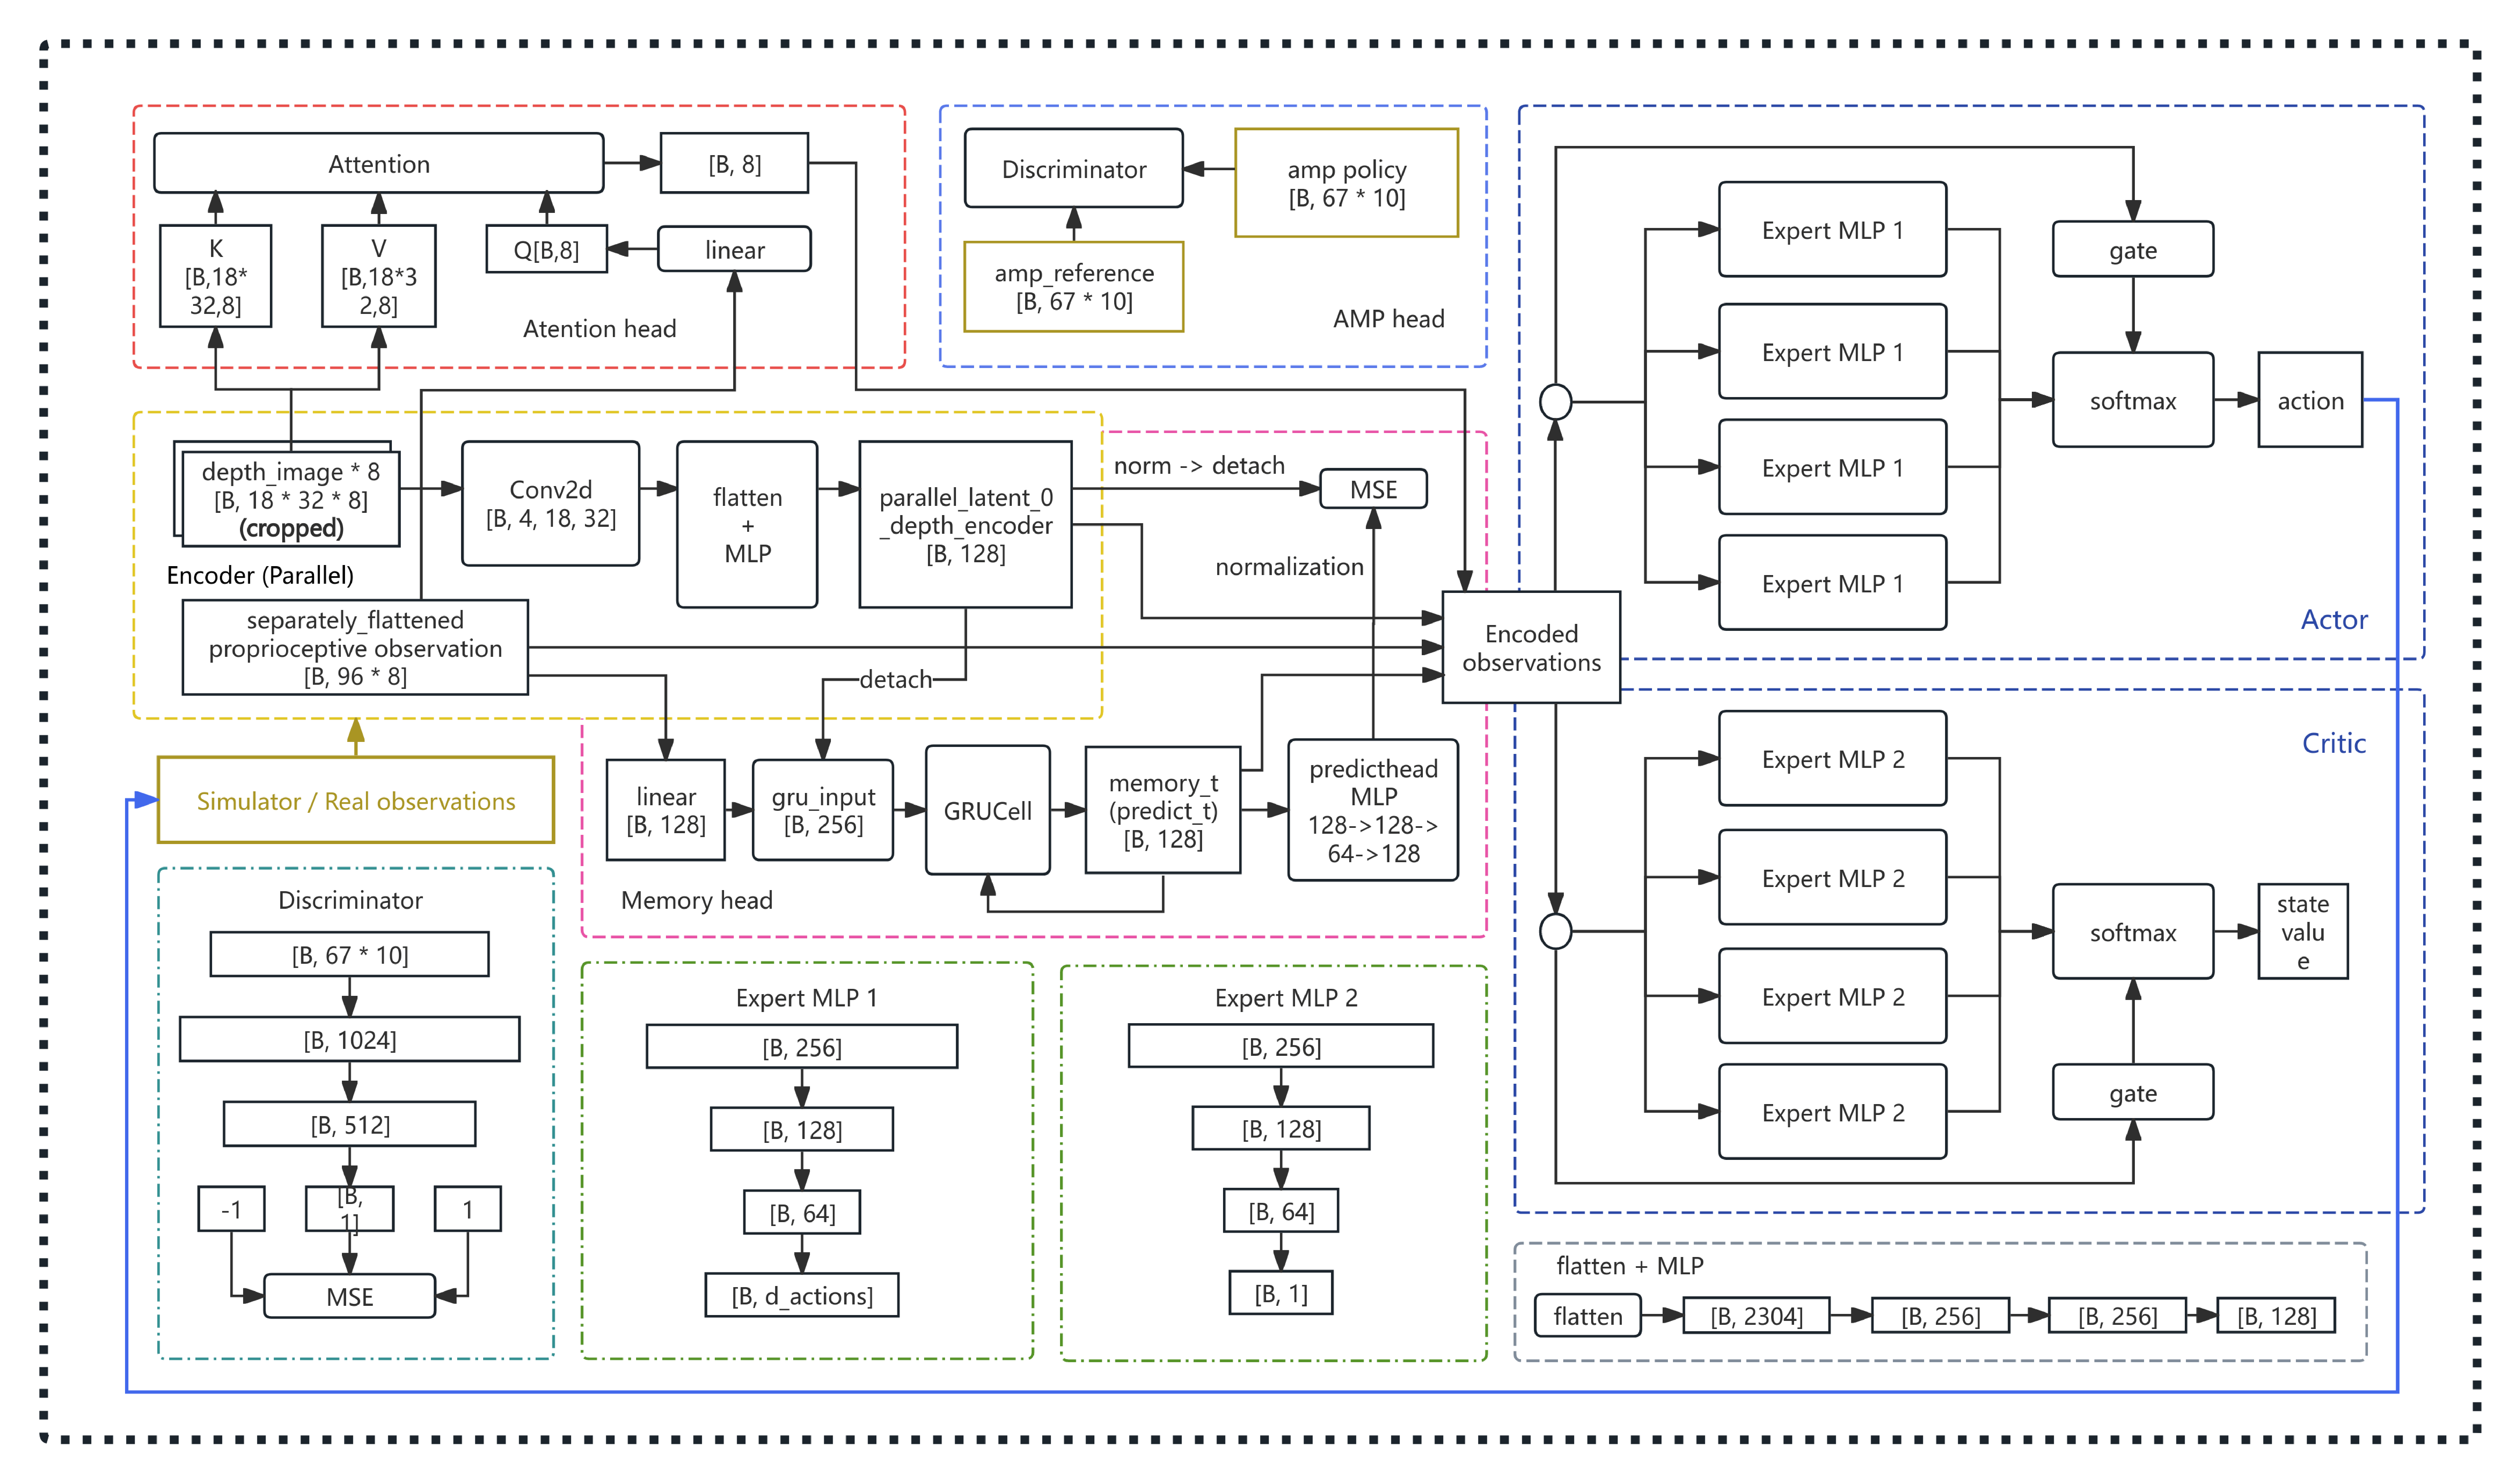
\includegraphics[width=\textwidth]{figures/ch3_overall_architecture.pdf}
    \caption{Overall architecture of the proposed framework. Proprioceptive observations and temporal-subsampled depth images are processed by the Memory-Attention Encoder, which produces four output streams: memory latent $\mathbf{m}_t$, attention latent $\mathbf{a}_t$, depth latent $\mathbf{z}_t^d$, and raw proprioceptive observations $\mathbf{o}_t^{\text{prop}}$. These are concatenated and fed into the MoE actor-critic, which outputs joint position targets. The AMP discriminator provides an adversarial style reward. The memory hidden state $\mathbf{h}_t$ is maintained across time steps and reset at episode boundaries.}
    \label{fig:overall_architecture}
\end{figure}

The key innovations of the proposed architecture are:

\begin{enumerate}
    \item \textbf{Temporal-subsampled depth image stack.} Rather than processing consecutive depth frames or a single frame, the proposed method samples depth images at fixed intervals (every 5 control steps) and stacks 8 sampled frames into a single multi-channel input. This design embeds temporal information into the spatial structure of the depth representation, allowing the convolutional encoder and attention module to jointly reason about spatial and temporal terrain features.

    \item \textbf{GRU memory with consistency loss.} A GRU cell maintains a hidden state that accumulates terrain information over time, enabling the policy to remember terrain features beyond the limited temporal window of the depth stack. A novel consistency loss ensures that the memory representation encodes meaningful terrain information by requiring the memory output to predict the current depth latent.

    \item \textbf{Cross-attention for spatial focus.} A multi-head cross-attention mechanism allows the policy to selectively focus on the most task-relevant regions of the depth image, using the robot's current proprioceptive state as a query. This enables adaptive spatial attention---for example, focusing on nearby obstacles when approaching a gap, or attending to wall structures when navigating confined spaces.

    \item \textbf{Mixture-of-Experts for skill routing.} Multiple expert networks with a learned gating mechanism enable the policy to specialize different expert sub-networks for different terrain types and locomotion skills, without requiring explicit skill decomposition or a high-level skill selector.

    \item \textbf{Adversarial motion priors with self-collected data.} The AMP module is trained on motion capture data collected by the authors and retargeted to the robot's morphology, covering walking, running, and stair-climbing motions that are directly relevant to parkour scenarios.
\end{enumerate}

The interaction between these components creates a complementary system: the memory module provides long-horizon terrain understanding (addressing the temporal dimension), the attention module provides spatial selectivity (addressing the spatial dimension), the MoE module provides skill diversity, and the AMP module provides motion style regularization. The temporal-subsampled depth stack serves as the perceptual foundation that bridges the memory and attention modules by encoding both spatial and temporal terrain features in a unified representation.

%% ============================================================
\section{Policy Input Representation}
\label{sec:policy_input}
%% ============================================================

The design of the policy input representation is critical for parkour: the observations must provide sufficient information for the policy to perceive terrain geometry, track velocity commands, and maintain awareness of the robot's internal state, while remaining compatible with real-time inference on onboard hardware. This section describes the two primary observation categories---proprioceptive observations and depth image observations---as well as the target-driven command system that guides the robot through the parkour course.

\subsection{Proprioceptive Observations}
\label{sec:proprio_obs}

The proprioceptive observation group provides the policy with information about the robot's internal state and the commanded velocities. To enable the policy to infer velocity and acceleration from position history, each scalar observation is repeated over a history window of $H=8$ consecutive time steps and flattened into a single vector. The proprioceptive observation components are listed in Table~\ref{tab:proprio_obs}.

\begin{table}[t]
\centering
\caption{Proprioceptive observation components for the policy. Each component is repeated over a history window of $H=8$ time steps. Additive uniform noise is applied during training for robustness.}
\label{tab:proprio_obs}
\footnotesize
\begin{tabular}{@{}lp{5.5cm}ccc@{}}
\toprule
\textbf{Component} & \textbf{Description} & \textbf{Dim.} & \textbf{Noise Range} & \textbf{Scale} \\
\midrule
Base angular velocity & Angular velocity in body frame & 3 & $[-0.2, 0.2]$ & 0.25 \\
Projected gravity & Gravity vector in body frame & 3 & $[-0.05, 0.05]$ & --- \\
Velocity commands & Target linear \& angular velocities & 3 & --- & --- \\
Joint positions (relative) & Current joint pos.\ minus default pos. & 29 & $[-0.01, 0.01]$ & --- \\
Joint velocities (relative) & Joint velocities & 29 & $[-0.5, 0.5]$ & 0.05 \\
Last action & Previous step's action output & 29 & --- & --- \\
\midrule
\textbf{Total per step} & & \textbf{96} & & \\
\textbf{Total with history} & $96 \times H$ & \textbf{768} & & \\
\bottomrule
\end{tabular}
\end{table}

The base angular velocity and projected gravity observations provide the policy with information about the robot's orientation and rotational dynamics. The velocity commands encode the target motion specified by the command system (described in Section~\ref{sec:target_command}). Joint positions and velocities provide the policy with fine-grained information about the robot's current pose and motion, enabling precise foot placement and whole-body coordination. The last action is included to enable the policy to produce smooth, temporally consistent actions by conditioning the current action on the previous one.

Additive uniform noise is applied to the proprioceptive observations during training to improve robustness to sensor noise and calibration errors at deployment. The noise ranges are chosen to be larger than the expected sensor noise in simulation but smaller than the signal magnitude, ensuring that the policy learns to be robust without losing information.

For the critic network, an additional observation group is provided that includes the base linear velocity (3 dimensions, repeated over $H=8$ steps for a total of 24 additional dimensions). This privileged information is available to the critic during training but not to the actor at deployment, following the asymmetric actor-critic paradigm that has been shown to improve training efficiency in locomotion tasks~\cite{zhang2024rpl}.

\subsection{Depth Image Observations}
\label{sec:depth_obs}

The depth image observation is the primary source of exteroceptive information for the policy, providing a direct measurement of the terrain geometry in front of the robot. Unlike height scanners that cast rays downward to produce a one-dimensional height profile~\cite{zhang2024rpl,cheng2024extremeparkour}, depth cameras provide a two-dimensional image that captures both the horizontal and vertical structure of the terrain, including walls, overhangs, and obstacles at varying distances.

\subsubsection{Sensor Configuration}

The depth camera is mounted on the robot's torso link, providing a first-person perspective of the terrain ahead. The camera has a horizontal field of view (FOV) of $87.5^\circ$ and a vertical FOV of $58.3^\circ$, with a resolution of $64 \times 36$ pixels. The depth measurements are clipped to a maximum range and normalized to the range $[0, 1]$ based on a depth range of $[0, 2.5]$~m, with a minimum distance of $0.1$~m. The camera update period is $20$~ms, corresponding to the control frequency of the policy.

\subsubsection{Temporal-Subsampled Depth Image Stack}
\label{sec:temporal_subsample}

A key innovation of the proposed framework is the temporal-subsampled depth image stack. Rather than processing consecutive depth frames (which would provide redundant information due to the high frame rate relative to the control frequency) or a single frame (which would lack temporal context), the proposed method samples depth images at fixed intervals and stacks the sampled frames into a multi-channel input.

Specifically, the depth observation function maintains a history buffer of the most recent depth frames. Every $S=5$ control steps, one frame is sampled from the buffer and appended to the output stack. The output stack contains $F=8$ frames, covering a total temporal span of:
\begin{equation}
    T_{\text{coverage}} = S \times F \times \Delta t = 5 \times 8 \times 0.02 = 0.8~\text{s}
\end{equation}
where $\Delta t = 0.02$~s is the control period. This design embeds temporal information into the spatial structure of the depth representation: each of the 8 channels in the depth stack corresponds to a different time step, allowing the convolutional encoder and attention module to jointly reason about spatial and temporal terrain features.

\begin{figure}[t]
    \centering
    
\includegraphics[width=0.85\textwidth]{figures/ch3_temporal_subsample.pdf}
    \caption{Illustration of the temporal-subsampled depth image stack. Consecutive depth frames (top row) are sampled every $S=5$ steps, producing 8 frames that span approximately 0.8 seconds of terrain history. The sampled frames are stacked along the channel dimension to form the input to the depth encoder. Earlier frames (left) provide information about terrain the robot has already traversed, while later frames (right) provide information about upcoming terrain.}
    \label{fig:temporal_subsample}
\end{figure}

The motivation for this design arises from the observation that consecutive depth frames at the control frequency contain largely redundant information---the terrain does not change significantly between adjacent 20~ms steps. By subsampling at intervals of 5 steps, each frame in the stack captures a meaningfully different terrain state, providing the policy with a compact temporal summary of the terrain evolution. This is particularly important for parkour, where the robot must anticipate upcoming obstacles (e.g., a gap approaching from a distance) and remember terrain features it has already traversed (e.g., a step it has just climbed).

Compared to the height scanner representation used in RPL~\cite{zhang2024rpl} and Extreme Parkour~\cite{cheng2024extremeparkour}, the temporal-subsampled depth stack provides three advantages: (1)~it captures vertical terrain structure (walls, overhangs) that height scanners cannot represent; (2)~it provides temporal context through the multi-frame stack, enabling the policy to infer terrain dynamics; and (3)~it preserves the full 2D spatial structure of the depth image, enabling the attention module to perform spatially selective processing.

Compared to the single-frame depth processing used in Hiking in the Wild~\cite{zhu2024hiking} and Humanoid Parkour Learning~\cite{zhuang2024humanoidparkour}, the temporal-subsampled depth stack provides temporal context that single-frame processing cannot: the policy can observe how terrain features change across the 8 sampled frames, enabling it to distinguish between approaching and receding obstacles, estimate the speed of terrain changes, and accumulate information about the terrain ahead.

\subsubsection{Depth Noise Pipeline}

To bridge the sim-to-real gap in depth perception, a multi-stage noise pipeline is applied to the depth images during training:

\begin{enumerate}
    \item \textbf{Crop and Resize.} A rectangular region of the depth image is cropped (crop region: rows 18--34, columns 0--16, producing a $16 \times 16$ sub-image) and resized back to the original resolution. This simulates the limited field of view and resolution of real depth sensors.

    \item \textbf{Gaussian Blur.} A Gaussian blur with kernel size 3 and standard deviation $\sigma=1$ is applied to smooth the depth image, simulating the noise characteristics of real depth sensors that produce spatially correlated measurement errors.

    \item \textbf{Depth Normalization.} Raw depth values are normalized from the range $[0, 2.5]$~m to $[0, 1]$, providing a consistent input scale for the encoder regardless of the absolute depth range.
\end{enumerate}

Additionally, a random frame delay of 0--1 steps is applied to simulate the latency of real depth sensors, and additive Gaussian noise and depth artifact noise are applied during training for further robustness.

\subsection{Target-Driven Command System}
\label{sec:target_command}

The velocity commands that guide the robot through the parkour course are generated by a target-driven command system. Unlike fixed-velocity or random-velocity command systems used in previous locomotion work~\cite{rudin2016walk,margolis2024rapidlocomotion}, the proposed system computes velocity commands based on the direction and distance to a target position sampled on the terrain.

At the beginning of each episode and at regular resampling intervals, a target position is randomly sampled from a set of valid target positions on the terrain. The valid target positions are pre-computed flat patches on each sub-terrain, ensuring that the target is always reachable. The command system then computes:
\begin{equation}
    \mathbf{c}_t^{\text{vel}} = \begin{bmatrix} k_v \cdot \Delta x_t^b \\ k_v \cdot \Delta y_t^b \\ k_h \cdot \Delta \psi_t \end{bmatrix}
\end{equation}
where $\Delta x_t^b$ and $\Delta y_t^b$ are the target position coordinates in the robot's body frame, $\Delta \psi_t$ is the heading error to the target, and $k_v = 2.0$ and $k_h = 2.0$ are the velocity and heading control stiffness gains, respectively. The velocity commands are clamped to terrain-specific ranges (e.g., forward velocity $v_x \in [0.45, 1.0]$~m/s for rough terrain, $v_x \in [0.3, 0.8]$~m/s for stair terrain).

When the robot is within a threshold distance of the target ($d_t < 0.4$~m), the velocity commands are set to zero, indicating that the current target has been reached. A proportion of environments are designated as ``standing'' environments where the velocity commands are always zero, encouraging the policy to learn stable standing behavior.

This target-driven command system provides a natural curriculum for parkour learning: the robot must navigate toward specific goal positions across diverse terrain, requiring it to develop terrain-appropriate locomotion strategies (e.g., stepping carefully on stairs, leaping across gaps, slowing down near walls) rather than simply moving at a fixed speed.

%% ============================================================
\section{Memory Module}
\label{sec:memory_module}
%% ============================================================

\subsection{Motivation}

Parkour locomotion requires the policy to maintain a persistent understanding of the terrain beyond the limited temporal window of the depth image stack. While the temporal-subsampled depth stack (Section~\ref{sec:temporal_subsample}) provides terrain information spanning approximately 0.8 seconds, many parkour scenarios demand longer-horizon terrain memory: the robot must remember that it has just climbed a step (to adjust its posture accordingly), recall the location of a gap it observed several seconds ago (to plan its approach), or maintain awareness of the overall terrain profile (to select appropriate locomotion strategies).

Existing approaches to memory in locomotion policies rely primarily on recurrent neural networks (RNNs) with implicit hidden states. DreamWaQ~\cite{nahraendra2024dreamwaq} uses an RNN hidden state as an implicit terrain imagination, but this representation is not explicitly supervised and may not encode terrain information in a structured or interpretable manner. LocoFormer~\cite{liu2024locoformer} uses a Transformer architecture with self-attention over observation sequences, but the quadratic complexity of self-attention limits the sequence length that can be processed in real time. Neither approach provides an explicit mechanism to ensure that the memory representation encodes meaningful terrain information.

The proposed memory module addresses these limitations through two design choices: (1)~a GRU cell that maintains a compact hidden state updated at each time step, providing a fixed-cost recurrent memory that can persist information over arbitrarily long horizons; and (2)~a consistency loss that explicitly supervises the memory representation to encode terrain information relevant to the current observation, ensuring that the memory state carries meaningful semantic content rather than degenerating into an uninterpretable latent code.

\subsection{Network Architecture}

The memory module operates on two inputs: the raw proprioceptive observations $\mathbf{o}_t^{\text{prop}}$ and the depth latent $\mathbf{z}_t^d$ produced by the depth encoder (described in Section~\ref{sec:depth_obs}). The architecture is as follows:

\begin{enumerate}
    \item \textbf{State projection.} The proprioceptive observations are projected through a linear layer:
    \begin{equation}
        \mathbf{s}_t = W_s \mathbf{o}_t^{\text{prop}} + \mathbf{b}_s, \quad \mathbf{s}_t \in \mathbb{R}^{128}
    \end{equation}
    where $W_s \in \mathbb{R}^{128 \times d_{\text{prop}}}$ and $\mathbf{b}_s \in \mathbb{R}^{128}$ are learnable parameters.

    \item \textbf{Input concatenation.} The projected state is concatenated with the \emph{detached} depth latent:
    \begin{equation}
        \mathbf{x}_t^{\text{mem}} = [\mathbf{s}_t \, \| \, \text{sg}(\mathbf{z}_t^d)], \quad \mathbf{x}_t^{\text{mem}} \in \mathbb{R}^{256}
    \end{equation}
    where $\text{sg}(\cdot)$ denotes the stop-gradient operator that prevents gradients from flowing through the depth latent into the memory input. This detachment is critical: it ensures that the memory module does not interfere with the depth encoder's training signal, allowing the two modules to be trained independently while still providing the memory with terrain information.

    \item \textbf{GRU update.} The concatenated input is fed into a GRU cell that updates the memory hidden state:
    \begin{equation}
        \mathbf{h}_t = \text{GRUCell}(\mathbf{x}_t^{\text{mem}}, \mathbf{h}_{t-1}), \quad \mathbf{h}_t \in \mathbb{R}^{128}
    \end{equation}
    The GRU cell uses gated updates with reset and update gates to selectively incorporate new information and retain relevant past information. The hidden size of 128 provides a compact representation that is sufficient for encoding terrain features while remaining computationally efficient for real-time inference.

    \item \textbf{Memory output.} The updated hidden state $\mathbf{h}_t$ serves as the memory latent $\mathbf{m}_t = \mathbf{h}_t$, which is concatenated with the other encoder outputs and fed into the MoE actor-critic.
\end{enumerate}

The memory hidden state is maintained across time steps during both training and inference. At episode boundaries (when a done signal is received), the hidden state is reset to zero for the corresponding environments. During training, the hidden states are stored in the rollout buffer and passed to the encoder during the policy update phase, enabling proper backpropagation through time (BPTT) across the stored trajectory segments.

\begin{figure}[t]
    \centering
    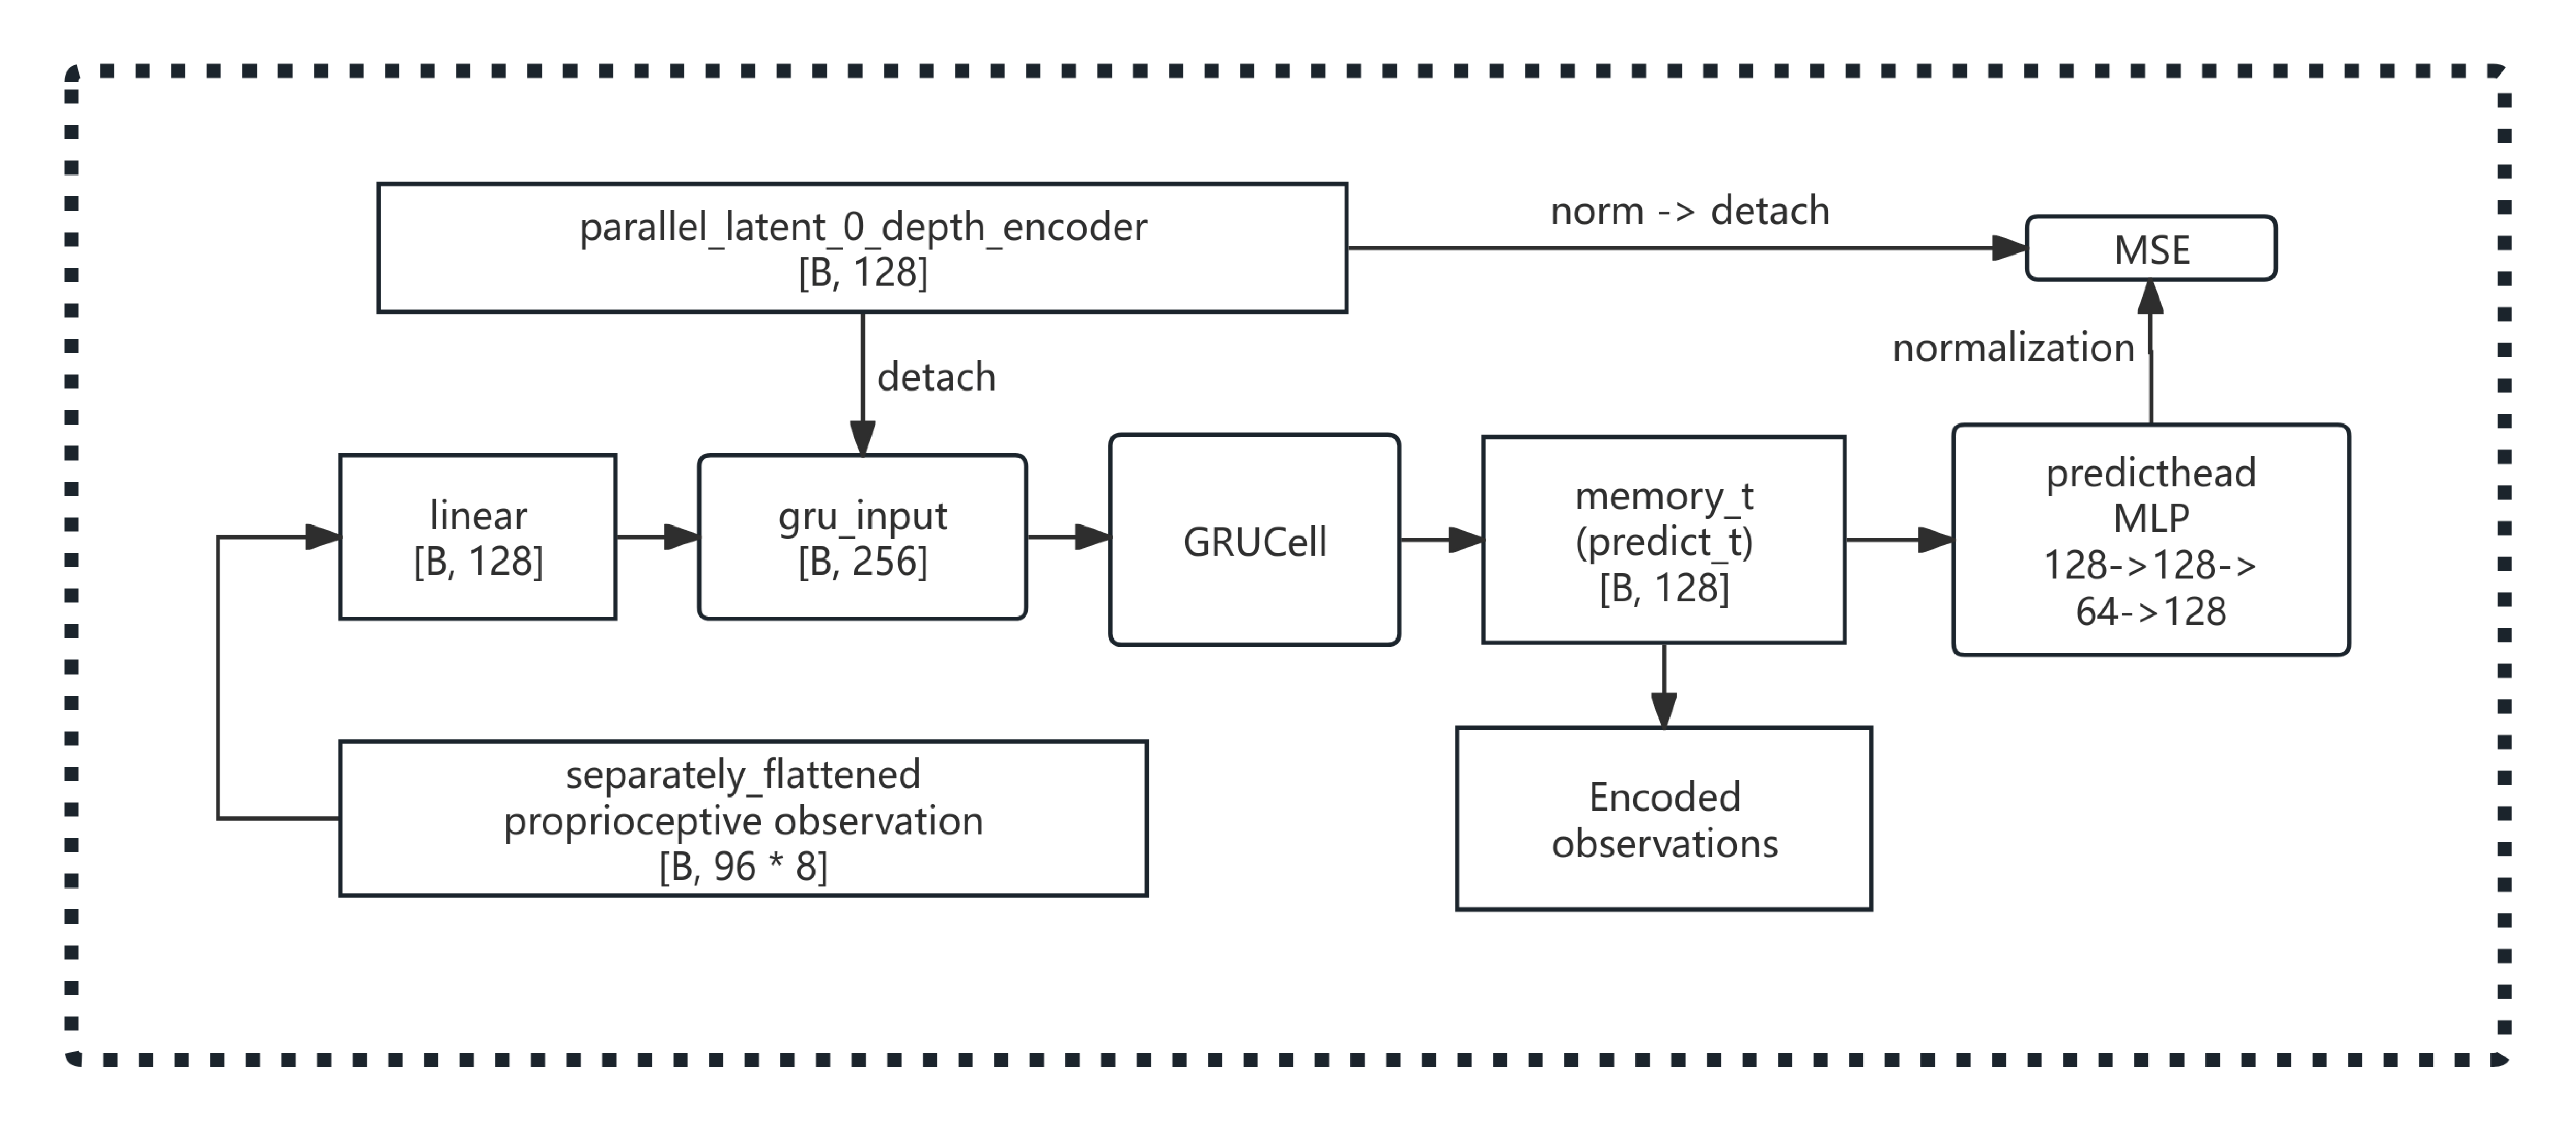
\includegraphics[width=0.85\textwidth]{figures/ch3_memory_module.pdf}
    \caption{Architecture of the memory module. The proprioceptive observations are projected to 128 dimensions and concatenated with the detached depth latent (128 dimensions) to form a 256-dimensional input to the GRU cell. The GRU hidden state (128 dimensions) is maintained across time steps and serves as the memory latent output. The consistency head produces a prediction target from the memory state, which is compared against the depth latent via the consistency loss.}
    \label{fig:memory_module}
\end{figure}

\subsection{Memory Consistency Loss}
\label{sec:consistency_loss}

A key challenge in training recurrent memory modules for locomotion is ensuring that the hidden state encodes meaningful information. Without explicit supervision, the GRU hidden state may degenerate into a representation that is useful for the policy's action selection but does not encode interpretable terrain features. This can lead to fragile memory representations that fail to generalize to new terrain configurations.

The proposed framework addresses this challenge through a \emph{memory consistency loss} that supervises the memory representation to predict the current depth latent. The consistency head is a multi-layer perceptron (MLP) that maps the memory hidden state to the depth latent space:
\begin{equation}
    \hat{\mathbf{z}}_t^d = f_{\text{head}}(\mathbf{m}_t) = W_3 \, \text{ELU}(W_2 \, \text{ELU}(W_1 \mathbf{m}_t + \mathbf{b}_1) + \mathbf{b}_2) + \mathbf{b}_3
\end{equation}
where the hidden dimensions are $128 \rightarrow 128 \rightarrow 64 \rightarrow 128$, matching the depth latent dimension. The consistency loss is then:
\begin{equation}
    \mathcal{L}_{\text{cons}} = \text{MSE}\left(\frac{\hat{\mathbf{z}}_t^d}{\|\hat{\mathbf{z}}_t^d\|}, \, \frac{\text{sg}(\mathbf{z}_t^d)}{\|\text{sg}(\mathbf{z}_t^d)\|}\right)
    \label{eq:consistency_loss}
\end{equation}
where both the prediction and the target are L2-normalized before computing the MSE. The normalization ensures that the loss measures the directional agreement between the memory prediction and the depth latent, rather than their magnitudes. The stop-gradient on $\mathbf{z}_t^d$ prevents the consistency loss from affecting the depth encoder's training.

\paragraph{Design Rationale.}
The consistency loss was arrived at after an unsuccessful attempt to train the memory module with a \emph{future prediction} objective---predicting the depth latent 1 second into the future. This approach failed for three reasons: (1)~the learning signal was insufficient, as predicting a precise future state from a noisy current observation is inherently difficult; (2)~the robot's body pose changes dramatically over 1 second in parkour, making the target depth latent highly variable; and (3)~predicting a single future time point provides a sparse and discontinuous training signal.

The current design---predicting the \emph{current} depth latent from the memory state---addresses these issues. The current depth latent is a stable, well-defined target that provides a dense learning signal at every time step. The key insight is that by requiring the memory to predict the current depth representation, the consistency loss forces the memory to encode a terrain interpretation that is consistent with the current visual observation. This terrain interpretation persists in the GRU hidden state even after the visual observation has changed, providing the policy with a stable terrain representation that is grounded in but not limited to the current depth input.

The consistency loss is incorporated into the PPO training objective as an auxiliary loss:
\begin{equation}
    \mathcal{L}_{\text{total}} = \mathcal{L}_{\text{PPO}} + \lambda_{\text{cons}} \cdot \mathcal{L}_{\text{cons}}
\end{equation}
where $\lambda_{\text{cons}}$ is a weighting coefficient. The consistency loss is computed for both the actor and critic encoders (which share the same architecture but maintain separate hidden states), and the total consistency loss is the average of the two.

\subsection{Qualitative Behavioral Effects}
\label{sec:memory_effects}

The memory module produces two notable behavioral effects that demonstrate its role in terrain understanding:

\paragraph{Conservative initial behavior.}
At the beginning of each episode, the GRU hidden state is initialized to zero, meaning the memory has no terrain information. However, the velocity commands immediately require the robot to move forward. The policy resolves this conflict by adopting a conservative locomotion strategy in the first few steps: it lifts its feet significantly higher than normal, effectively ``stepping blind'' with elevated foot clearance. This behavior is not a training artifact but rather a rational strategy: when the memory is empty, the policy has no information about the terrain ahead and compensates by increasing the safety margin for foot placement. As the GRU accumulates terrain information over the first few steps, the foot clearance gradually decreases to a normal level.

\paragraph{Confident terrain-adapted locomotion.}
After the memory has accumulated sufficient terrain information (typically within 3--5 steps), the policy transitions to terrain-adapted locomotion: it walks smoothly and efficiently on flat terrain, steps precisely on stairs, and adjusts its gait proactively when approaching obstacles. This transition from conservative to confident behavior indicates that the memory module is effectively encoding and maintaining terrain information, and that the policy has learned to modulate its behavior based on the information content of the memory state.

These behavioral patterns provide qualitative evidence that the memory consistency loss successfully forces the GRU hidden state to encode meaningful terrain representations. Without the consistency loss, the GRU hidden state would be free to encode arbitrary information that is useful for action selection but not necessarily terrain-related, potentially leading to a memory representation that is brittle and fails to generalize.

%% ============================================================
\section{Attention Module}
\label{sec:attention_module}
%% ============================================================

\subsection{Motivation}

While the depth image provides comprehensive spatial information about the terrain, not all regions of the depth image are equally important for the current locomotion decision. When the robot is approaching a gap, the region immediately ahead of its feet is far more critical than the distant terrain; when navigating near a wall, the wall's position and orientation determine whether the robot should stop or turn; and when stepping onto a narrow foothold, the precise geometry of the foothold region requires more attention than the surrounding terrain.

Existing depth-based locomotion methods process the entire depth image uniformly through a convolutional encoder~\cite{zhu2024hiking,zhuang2024humanoidparkour}, treating all spatial regions with equal importance. This uniform processing has two limitations: (1)~computational resources are wasted on irrelevant terrain regions, and (2)~the encoder may fail to capture fine-grained features in critical regions because its capacity is spread across the entire image. He et al.~\cite{he2024attentionmap} demonstrated that attention-based terrain encoding can improve locomotion generalization by selectively focusing on the most relevant terrain features, but their approach processes a single heightmap observation and does not address the multi-frame, multi-modal setting of the proposed framework.

The proposed attention module addresses these limitations through a cross-attention mechanism that uses the robot's current proprioceptive state as a query to selectively attend to the most task-relevant regions of the depth image. This design enables the policy to dynamically adjust its spatial focus based on the current locomotion context---for example, attending to nearby obstacles when approaching a gap, or focusing on wall structures when navigating confined spaces.

\subsection{Network Architecture}

The attention module implements a cross-attention mechanism between the proprioceptive observations (query) and the depth image spatial features (key and value). The architecture is as follows:

\begin{enumerate}
    \item \textbf{Key/Value construction.} The depth observation tensor $\mathbf{D}_t \in \mathbb{R}^{F \times H_d \times W_d}$ (where $F=8$, $H_d=36$, $W_d=64$) is reshaped into a sequence of spatial feature vectors. Each spatial position $(h, w)$ in the depth image has an $F$-dimensional feature vector (one value per temporal frame), and the entire image produces $L = H_d \times W_d = 2304$ such vectors:
    \begin{equation}
        \mathbf{K}_t = \mathbf{V}_t = \text{reshape}(\text{permute}(\mathbf{D}_t)) \in \mathbb{R}^{L \times d_a}
    \end{equation}
    where $d_a = F = 8$ is the attention embedding dimension. The constraint that the attention embedding dimension equals the number of depth frames ensures that the depth features can be directly used as key/value vectors without an additional projection layer, reducing the parameter count.

    \item \textbf{Query construction.} The proprioceptive observations are projected to the attention embedding dimension:
    \begin{equation}
        \mathbf{q}_t = W_q \mathbf{o}_t^{\text{prop}} + \mathbf{b}_q, \quad \mathbf{q}_t \in \mathbb{R}^{d_a}
    \end{equation}
    The query is then unsqueezed to add a sequence dimension: $\mathbf{Q}_t = \mathbf{q}_t^{\top} \in \mathbb{R}^{1 \times d_a}$.

    \item \textbf{Multi-head cross-attention.} The query, key, and value are processed by a multi-head attention layer with $N_h = 2$ heads:
    \begin{equation}
        \text{Attn}(\mathbf{Q}_t, \mathbf{K}_t, \mathbf{V}_t) = \text{softmax}\left(\frac{\mathbf{Q}_t \mathbf{K}_t^\top}{\sqrt{d_a / N_h}}\right) \mathbf{V}_t
    \end{equation}
    The output is a single vector $\mathbf{a}_t \in \mathbb{R}^{d_a}$ obtained by squeezing the sequence dimension. The two attention heads enable the module to learn two distinct spatial attention patterns---for example, one head may specialize in attending to nearby terrain features (relevant for immediate foot placement), while the other may attend to distant terrain features (relevant for trajectory planning).
\end{enumerate}

\begin{figure}[t]
    \centering
    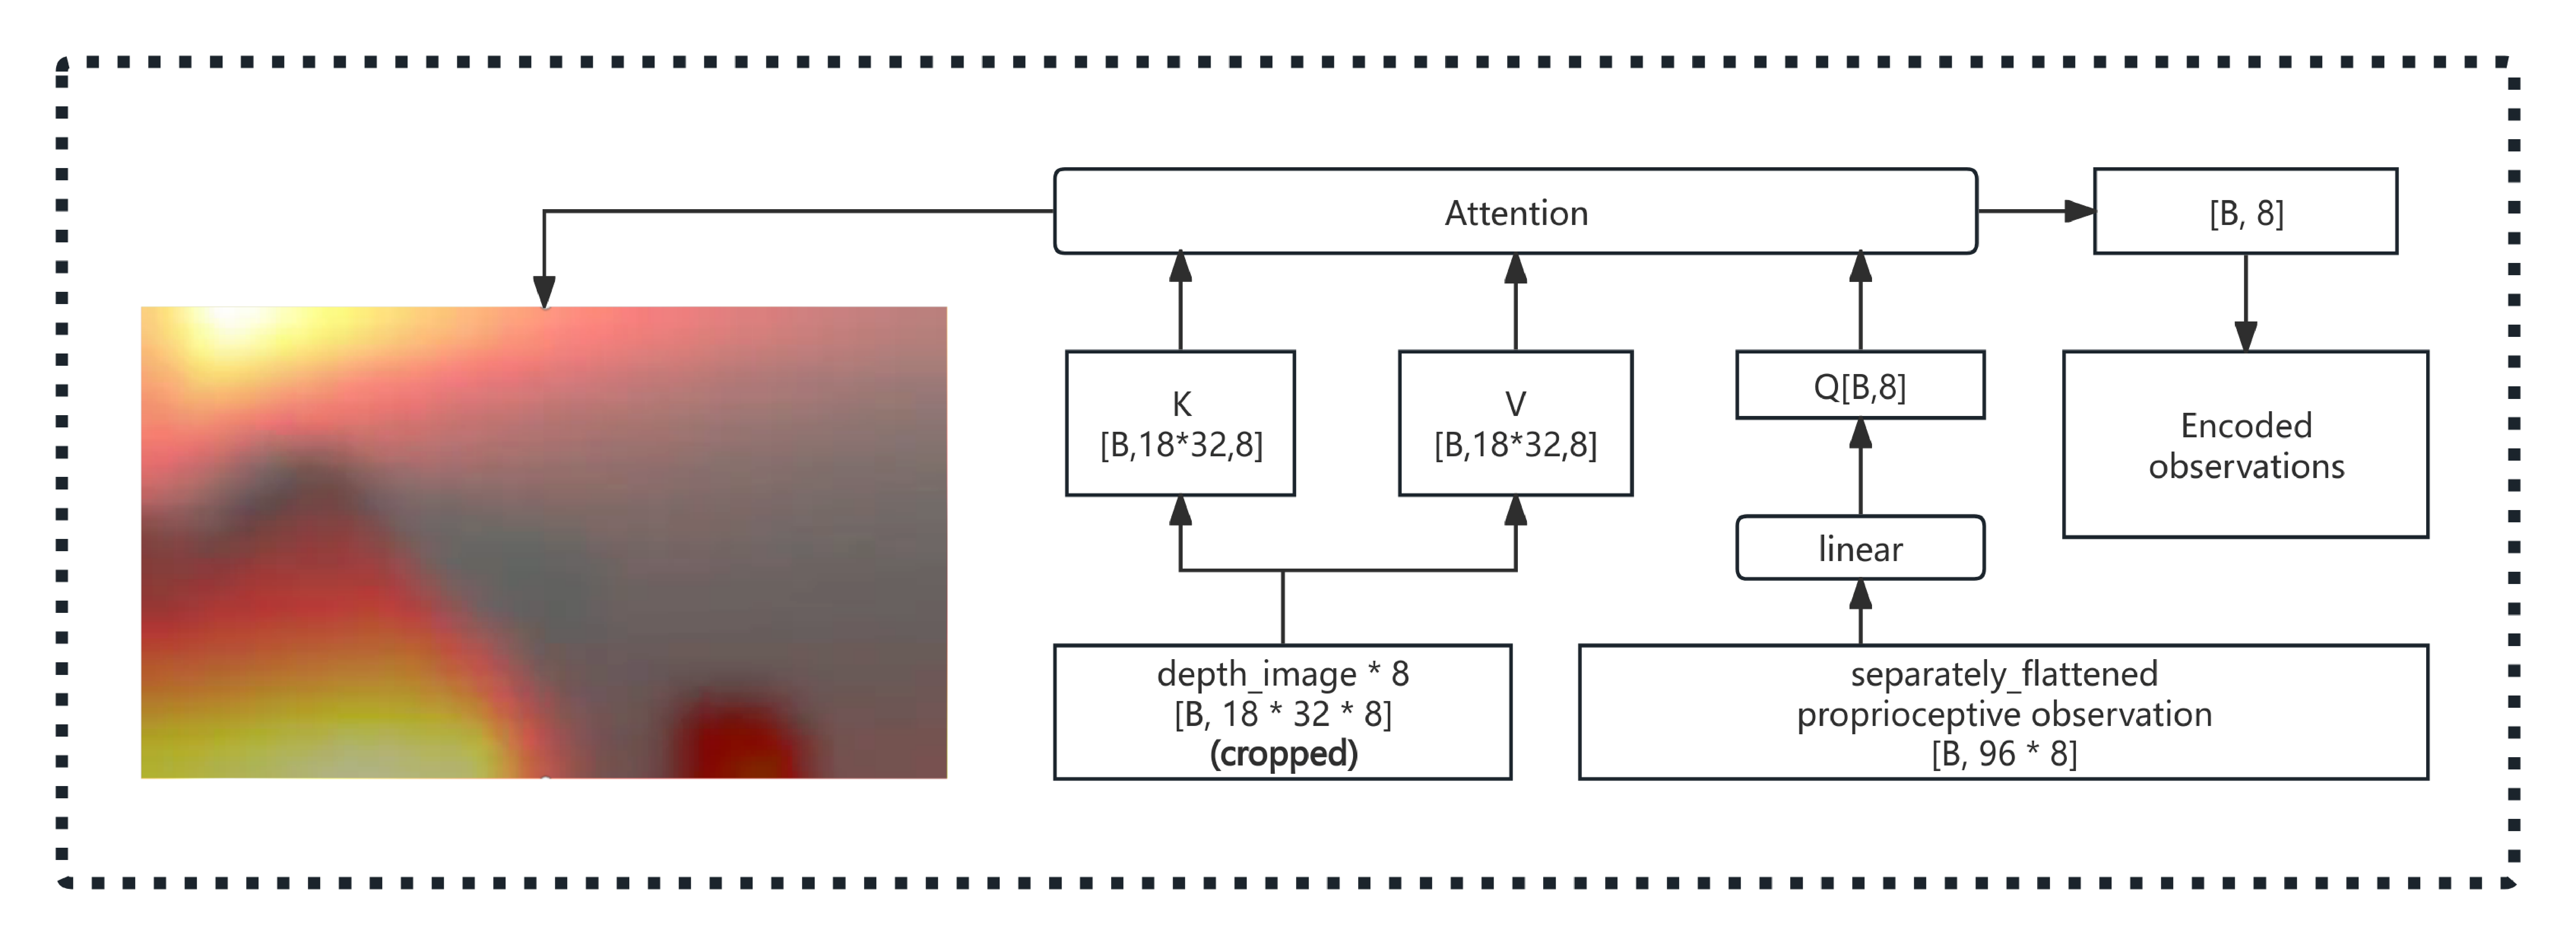
\includegraphics[width=0.85\textwidth]{figures/ch3_attention_module.pdf}
    \caption{Architecture of the cross-attention module. The depth image is reshaped into a sequence of $L = H_d \times W_d$ spatial feature vectors, each of dimension $d_a = F$ (the number of depth frames). The proprioceptive observations are projected to the same dimension and used as a query. Multi-head cross-attention (2 heads) produces an attention output $\mathbf{a}_t \in \mathbb{R}^{d_a}$. The attention weights can be reshaped back to the spatial dimensions of the depth image for visualization.}
    \label{fig:attention_module}
\end{figure}

The attention weights can be reshaped from $(N_h, 1, L)$ to $(N_h, H_d, W_d)$ to produce spatial attention maps over the depth image. These attention maps provide interpretable insights into which terrain regions the policy attends to when making locomotion decisions, enabling qualitative analysis of the policy's spatial focus.

\subsection{Qualitative Behavioral Effects}
\label{sec:attention_effects}

Visualization of the attention weights reveals that the policy learns meaningful spatial attention patterns that adapt to different terrain scenarios:

\paragraph{Obstacle avoidance.}
When the depth image contains obstacles that could affect the robot's posture or cause tripping, the attention weights concentrate on these obstacle regions. The policy learns to attend to the spatial extent and proximity of obstacles, enabling it to adjust its foot placement and body posture proactively rather than reactively. This is particularly important for small obstacles (e.g., stones, low steps) that occupy a small portion of the depth image but have a disproportionate impact on locomotion stability.

\paragraph{Wall avoidance.}
When the depth image shows a wall ahead, the attention weights focus on the wall region, and the policy learns to stop forward motion rather than colliding with the wall. This behavior demonstrates that the attention module enables the policy to recognize and respond to terrain features that require a qualitative change in locomotion strategy (from forward motion to stopping), rather than merely adjusting the parameters of a fixed locomotion pattern.

\paragraph{Two-stage gap crossing.}
For gap-crossing scenarios, the attention weights reveal a two-stage decision process. In the first stage, when the gap is still at a distance, the attention focuses on the gap's far edge, and the policy walks toward the gap edge (rather than attempting to leap from a distance). In the second stage, when the robot is at the gap edge, the attention shifts to the gap's geometry (width, depth), and the policy adjusts its center of mass and executes a large step to cross the gap. This two-stage behavior---approach then cross---is more robust than attempting to cross the gap from an arbitrary distance, as it ensures that the robot has optimal footing and balance before committing to the crossing maneuver.

\paragraph{Comparison with attention-free AMP-only policies.}
Policies trained with AMP but without the attention module exhibit a characteristic limitation: they learn natural locomotion postures through the AMP discriminator and basic obstacle avoidance through the depth encoder, but they fail to attend to small, localized terrain features such as stones or low steps near the robot's feet. This is a well-known limitation of current AMP-based locomotion methods---the AMP reward encourages natural motion style but does not provide the spatial selectivity needed to focus on critical terrain regions. The attention module addresses this limitation by enabling the policy to selectively amplify the representation of important terrain features, ensuring that even small obstacles receive sufficient processing capacity.

%% ============================================================
\section{Mixture-of-Experts Module}
\label{sec:moe_module}
%% ============================================================

\subsection{Motivation}

Parkour requires the robot to execute a diverse repertoire of locomotion skills---walking on flat terrain, climbing stairs, leaping across gaps, navigating slopes, and avoiding walls---often in rapid succession as the terrain changes. A single monolithic policy network may struggle to simultaneously master all these skills, as the optimal locomotion strategy for one terrain type may conflict with the optimal strategy for another (e.g., the high-step strategy for stairs vs.\ the low-swing strategy for flat walking).

Existing approaches to multi-skill parkour employ explicit skill decomposition: Extreme Parkour~\cite{cheng2024extremeparkour} and Robot Parkour Learning~\cite{zhuang2024robotparkour} train separate skill policies for each maneuver type and use a high-level planner to select and parameterize skills. While effective, this skill-chaining paradigm requires manual skill definition, careful skill boundary design, and a separate high-level policy, increasing the engineering complexity and limiting the system's ability to learn novel skill combinations.

The proposed framework employs a Mixture-of-Experts (MoE) architecture as an alternative to explicit skill decomposition. In the MoE paradigm, the policy network contains multiple expert sub-networks, each of which can specialize in a different locomotion strategy, and a gating network that dynamically selects which experts to activate for each input. This design enables the policy to learn diverse locomotion skills end-to-end without requiring explicit skill labels or a high-level skill selector.

\subsection{Network Architecture}

The MoE module replaces the standard MLP actor and critic heads with MoE layers. Each MoE layer consists of two components:

\begin{enumerate}
    \item \textbf{Gating network.} A linear layer maps the input to a distribution over experts:
    \begin{equation}
        \mathbf{g}_t = \text{softmax}(W_g \mathbf{x}_t + \mathbf{b}_g), \quad \mathbf{g}_t \in \mathbb{R}^{N_e}
    \end{equation}
    where $N_e = 8$ is the number of experts. The gate scores $\mathbf{g}_t$ represent the relative importance of each expert for the current input.

    \item \textbf{Expert networks.} Each expert $e$ is an MLP with hidden dimensions $[256, 256, 256]$ and an output dimension matching the action space (for the actor) or value space (for the critic). All experts share the same architecture but have independent parameters.

    \item \textbf{Weighted mixing.} The expert outputs are combined according to the gate scores:
    \begin{equation}
        \mathbf{y}_t = \sum_{e=1}^{N_e} g_{t,e} \cdot \mathbf{y}_{t,e} = \sum_{e=1}^{N_e} g_{t,e} \cdot f_e(\mathbf{x}_t)
    \end{equation}
    where $f_e$ is the $e$-th expert network and $g_{t,e}$ is the gate score for expert $e$ at time $t$. This soft mixing allows multiple experts to contribute to the output, enabling smooth interpolation between specialized strategies.
\end{enumerate}

\begin{figure}[t]
    \centering
    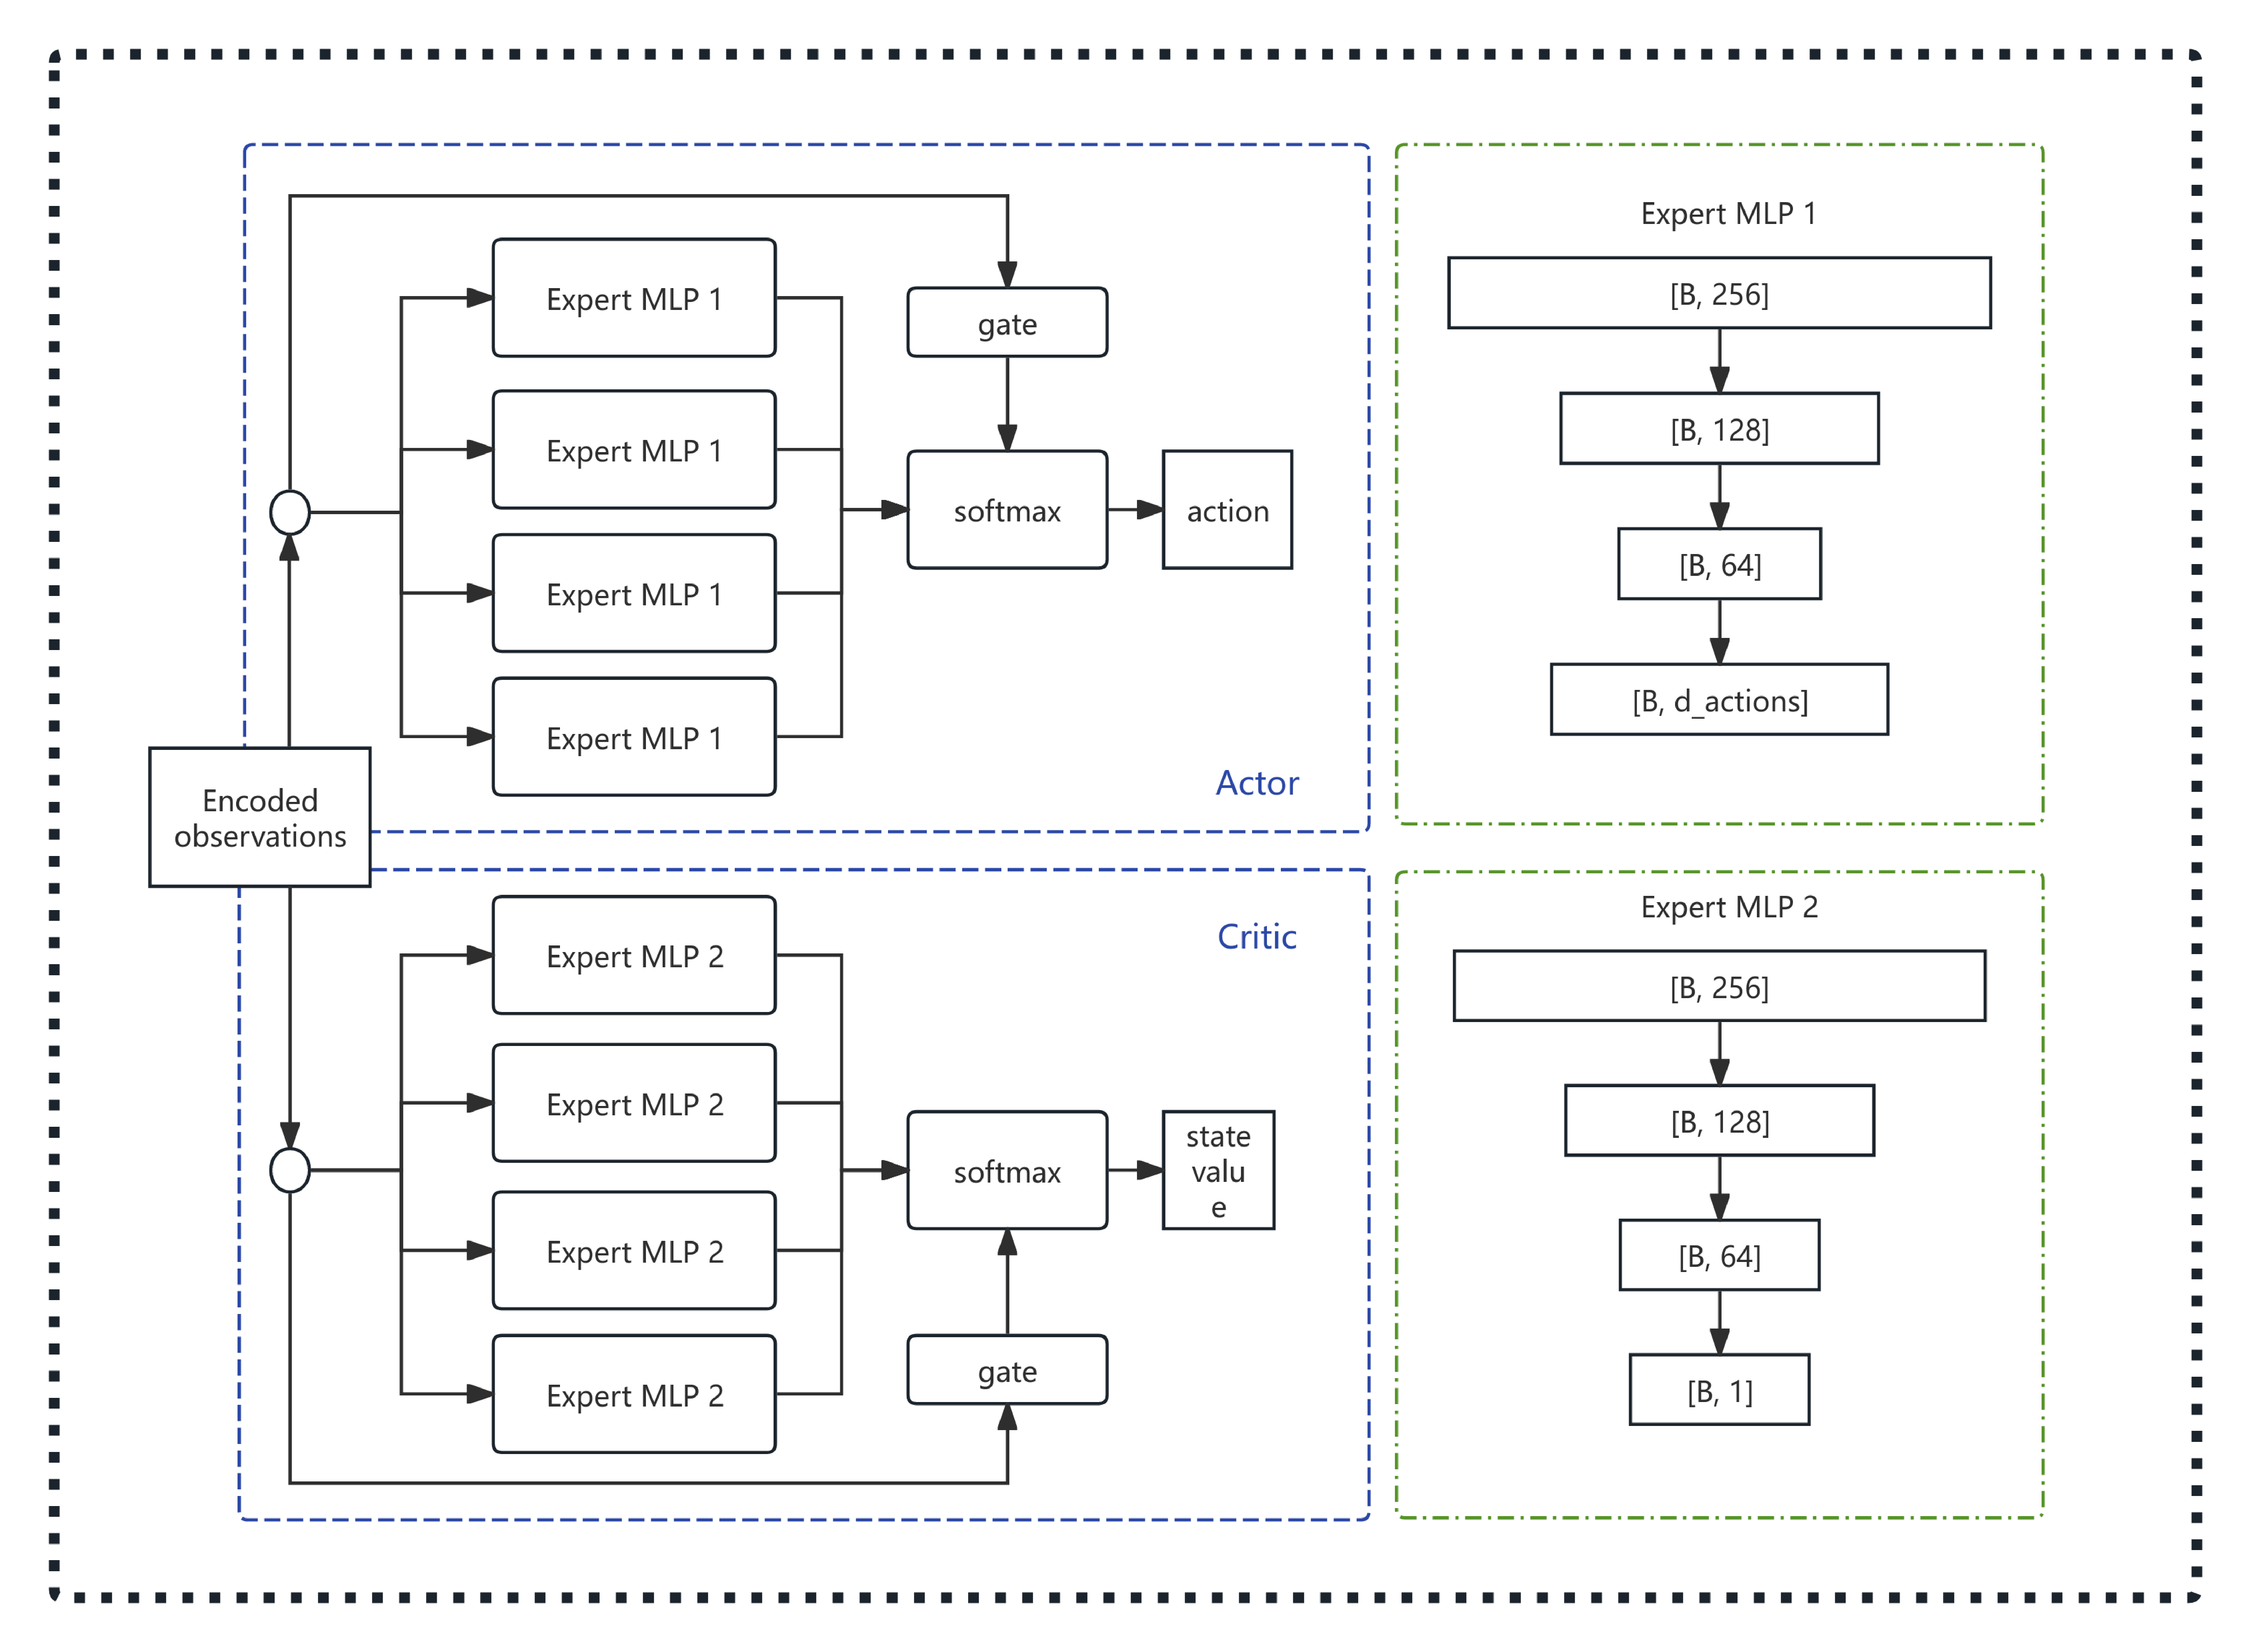
\includegraphics[width=0.75\textwidth]{figures/ch3_moe_module.pdf}
    \caption{Architecture of the Mixture-of-Experts layer. The input $\mathbf{x}_t$ is processed by a gating network that produces a softmax distribution over $N_e = 8$ experts. Each expert is an MLP with hidden dimensions $[256, 256, 256]$. The expert outputs are combined by weighted summation according to the gate scores. Both the actor and critic heads use independent MoE layers.}
    \label{fig:moe_module}
\end{figure}

The actor and critic each use an independent MoE layer with separate gating networks and expert parameters. This allows the actor and critic to develop different expert specializations: the actor's experts may specialize in different locomotion strategies (e.g., one expert for high-step climbing, another for flat walking), while the critic's experts may specialize in evaluating different terrain types.

\subsection{Comparison with Skill-Chaining Approaches}

The MoE architecture offers several advantages over the skill-chaining paradigm used in Extreme Parkour~\cite{cheng2024extremeparkour} and Robot Parkour Learning~\cite{zhuang2024robotparkour}:

\begin{enumerate}
    \item \textbf{No manual skill definition.} The MoE module does not require pre-defined skill categories or skill-specific reward functions. The expert specializations emerge automatically during training, driven by the diversity of the training terrain and the overall reward structure.

    \item \textbf{Smooth skill transitions.} The soft mixing of expert outputs enables smooth transitions between locomotion strategies, avoiding the discontinuities that can arise when switching between discrete skill policies.

    \item \textbf{End-to-end training.} The entire policy---including the encoder, MoE heads, and gating network---is trained jointly with a single PPO objective, simplifying the training pipeline compared to the multi-stage training required for skill-chaining approaches.

    \item \textbf{Scalability.} Adding more experts increases the model's capacity without changing the inference cost per expert, as each expert is evaluated independently. The gate computation adds negligible overhead.
\end{enumerate}

The primary limitation of the MoE approach is that the expert specializations are not guaranteed to be interpretable or well-separated: multiple experts may learn similar strategies, or a single expert may dominate the gate scores. However, the soft mixing mechanism mitigates this concern by ensuring that the output is always a reasonable combination of expert opinions, even if the expert specializations are not perfectly distinct.

%% ============================================================
\section{Adversarial Motion Prior Module}
\label{sec:amp_module}
%% ============================================================

\subsection{Motivation}

Reinforcement learning policies trained with pure task rewards often produce locomotion behaviors that are functionally correct but visually unnatural---the robot may shuffle its feet, exhibit jerky joint motions, or adopt awkward body postures that achieve the task objective but are energetically inefficient and potentially damaging to the hardware. In parkour scenarios, this problem is particularly acute because the diverse terrain types encourage the policy to adopt a wide range of locomotion strategies, some of which may be functional but physically implausible.

Adversarial Motion Priors (AMP)~\cite{peng2021amp} provide a principled solution to this problem by training a discriminator network that distinguishes between the policy's motion (``fake'') and reference motion data (``real''). The policy receives an adversarial reward that encourages it to produce motions that are indistinguishable from the reference data, effectively learning a style prior that regularizes the task-driven policy toward natural, human-like motion.

\subsection{AMP Framework}

The AMP module consists of a discriminator network $D_\phi$ that is trained concurrently with the policy. The discriminator receives a window of motion features and outputs a probability that the motion is ``real'' (from the reference dataset) rather than ``fake'' (from the policy). The AMP reward for the policy is:
\begin{equation}
    r_t^{\text{AMP}} = -\log(1 - D_\phi(\mathbf{s}_t^{\text{amp}})) + \log(D_\phi(\mathbf{s}_t^{\text{ref}}))
\end{equation}
where $\mathbf{s}_t^{\text{amp}}$ denotes the motion features from the policy and $\mathbf{s}_t^{\text{ref}}$ denotes the motion features from the reference dataset. The discriminator is trained to maximize its classification accuracy, while the policy is trained to maximize the AMP reward (i.e., to fool the discriminator).

\subsection{Observation Groups for AMP}

The AMP discriminator processes two observation groups with identical structure but different data sources:

\begin{table}[t]
\centering
\caption{AMP observation components for both the policy (amp\_policy) and reference (amp\_reference) groups. Each component is repeated over a history window of $H_{\text{amp}}=10$ time steps.}
\label{tab:amp_obs}
\begin{tabular}{llc}
\toprule
\textbf{Component} & \textbf{Description} & \textbf{Dim. per step} \\
\midrule
Projected gravity & Gravity vector in body frame & 3 \\
Joint positions (relative) & Current joint pos.\ minus default pos. & 29 \\
Joint velocities (relative) & Joint velocities (scaled by 0.05) & 29 \\
Base linear velocity & Linear velocity in body frame & 3 \\
Base angular velocity & Angular velocity in body frame & 3 \\
\midrule
\textbf{Total per step} & & \textbf{67} \\
\textbf{Total with history} & $67 \times H_{\text{amp}}$ & \textbf{670} \\
\bottomrule
\end{tabular}
\end{table}

The \texttt{amp\_policy} observation group samples motion features from the policy's current trajectory, while the \texttt{amp\_reference} observation group samples motion features from the retargeted reference dataset. The reference dataset consists of self-collected motion capture data of walking, running, and stair-climbing motions, retargeted to the robot's morphology using a general motion retargeting method~\cite{araujo2024retargeting}. The data collection and retargeting process is described in detail in Chapter~4.

\subsection{Integration with PPO Training}

The AMP reward is combined with the task reward to form the total reward signal for PPO training:
\begin{equation}
    r_t = r_t^{\text{task}} + w_{\text{AMP}} \cdot r_t^{\text{AMP}}
\end{equation}
where $w_{\text{AMP}}$ is a weighting coefficient that balances the task objective and the motion style objective. The discriminator is updated concurrently with the policy using a separate Adam optimizer, following the standard AMP training procedure~\cite{peng2021amp}.

The AMP discriminator is trained with a gradient penalty to prevent it from becoming overly confident, which could lead to vanishing gradients for the policy. The discriminator loss is:
\begin{equation}
    \mathcal{L}_D = -\mathbb{E}[\log D_\phi(\mathbf{s}^{\text{ref}})] - \mathbb{E}[\log(1 - D_\phi(\mathbf{s}^{\text{amp}}))] + \lambda_{\text{gp}} \cdot \mathcal{L}_{\text{gp}}
\end{equation}
where $\mathcal{L}_{\text{gp}}$ is the gradient penalty term and $\lambda_{\text{gp}}$ is its weighting coefficient.

\subsection{Comparison with Existing AMP Applications}

Most existing AMP-based locomotion methods~\cite{peng2021amp,zhang2024advdiscriminators} use publicly available motion capture datasets (e.g., AMASS) that primarily contain walking and running on flat ground. While these datasets provide a good style prior for flat-terrain locomotion, they lack the diversity of motion patterns needed for parkour---stair climbing, high-stepping, cautious approach walking, and dynamic leaping are not well-represented in standard motion capture datasets.

The proposed framework addresses this limitation by using self-collected motion capture data that specifically targets parkour-relevant motions. The reference dataset includes walking, running, and stair-climbing motions captured from human actors using a motion capture system, and retargeted to the robot's morphology using a general motion retargeting method~\cite{araujo2024retargeting}. This ensures that the AMP discriminator provides a style prior that is both natural (grounded in real human motion) and relevant (covering the motion patterns needed for parkour). The retargeting process accounts for differences in body proportions and joint limits between the human actor and the robot, producing reference motions that are feasible for the robot's embodiment.

Furthermore, the proposed framework applies symmetric augmentation to the reference dataset: each reference motion is mirrored left-to-right using a joint mapping that swaps corresponding left and right joints. This doubles the effective size of the reference dataset and encourages the AMP discriminator to learn symmetric motion patterns, which is important for bipedal locomotion where left and right steps should be stylistically similar.

%% ============================================================
\section{Implementation Details}
\label{sec:implementation}
%% ============================================================

This section describes the implementation details of the proposed framework, including the reward function design, environment configuration, sensor randomization, domain randomization, and training procedure. These details are critical for reproducibility and for understanding the design choices that differentiate the proposed method from ablation variants.

\subsection{Reward Function Design}
\label{sec:reward_function}

The reward function is composed of three categories: task rewards that encourage goal-directed behavior, regularization rewards that promote smooth and efficient motion, and safety rewards that prevent dangerous states. The complete reward function is listed in Table~\ref{tab:reward_terms}.

\begin{table}[t]
\centering
\caption{Complete reward function components. Positive weights indicate rewards, negative weights indicate penalties.}
\label{tab:reward_terms}
\footnotesize
\begin{tabular}{@{}lp{3.2cm}rp{7cm}@{}}
\toprule
\textbf{Category} & \textbf{Term} & \textbf{Weight} & \textbf{Description} \\
\midrule
\multirow{6}{*}{Task} & track\_lin\_vel\_xy & $+2.0$ & Track commanded linear velocity (exp.\ kernel, $\sigma=0.5$) \\
 & track\_ang\_vel\_z & $+2.0$ & Track commanded angular velocity (exp.\ kernel, $\sigma=0.5$) \\
 & heading\_error & $-1.0$ & Penalize heading deviation from command \\
 & dont\_wait & $-0.5$ & Penalize standing still when forward command is active \\
 & is\_alive & $+3.0$ & Reward for surviving each step \\
 & stand\_still & $-0.3$ & Penalize moving when no command (offset=4.0) \\
\midrule
\multirow{12}{*}{Regularization} & volume\_points\_penetration & $-4.0$ & Penalize foot volume penetrating virtual obstacles \\
 & feet\_air\_time & $+0.5$ & Reward swing foot air time (bipedal stepping) \\
 & feet\_slide & $-0.4$ & Penalize foot sliding on contact (threshold=1.0) \\
 & joint\_deviation\_hip & $-0.5$ & Penalize hip yaw/roll deviation from default \\
 & ang\_vel\_xy\_l2 & $-0.05$ & Penalize base roll/pitch angular velocity \\
 & dof\_torques\_l2 & $-1.5 \times 10^{-7}$ & Penalize joint torques (hip, knee, ankle) \\
 & dof\_acc\_l2 & $-1.25 \times 10^{-7}$ & Penalize joint accelerations \\
 & dof\_vel\_l2 & $-1.0 \times 10^{-4}$ & Penalize joint velocities \\
 & action\_rate\_l2 & $-0.005$ & Penalize action change between steps \\
 & flat\_orientation\_l2 & $-3.0$ & Penalize base orientation deviation from horizontal \\
 & pelvis\_orientation\_l2 & $-3.0$ & Penalize pelvis orientation deviation \\
 & feet\_flat\_ori & $-0.4$ & Penalize foot orientation misalignment on contact \\
\midrule
\multirow{7}{*}{Regularization (cont.)} & feet\_at\_plane & $-0.1$ & Penalize foot height error vs.\ terrain plane \\
 & feet\_close\_xy & $+0.4$ & Reward feet at appropriate lateral distance ($\sigma^2=0.05$) \\
 & energy & $-5.0 \times 10^{-5}$ & Penalize mechanical power (torque$\times$velocity) \\
 & freeze\_upper\_body & $-0.004$ & Penalize upper body joint deviation (L1 norm) \\
\midrule
\multirow{4}{*}{Safety} & dof\_pos\_limits & $-1.0$ & Penalize joint position limit violations \\
 & dof\_vel\_limits & $-1.0$ & Penalize joint velocity limit violations (soft ratio=0.9) \\
 & torque\_limits & $-0.01$ & Penalize torque exceeding 80\% of limit \\
 & undesired\_contacts & $-1.0$ & Penalize non-foot contact forces $>1.0$~N \\
\bottomrule
\end{tabular}
\end{table}

Several reward terms warrant additional discussion:

\paragraph{Volume points penetration.}
This term is a key safety mechanism for parkour. A set of 3D sample points is generated around each ankle in a grid pattern ($10 \times 5 \times 2$ points, spanning a volume of $0.15 \times 0.06 \times 0.04$~m around the foot). These points are checked against virtual obstacles generated from the terrain mesh (specifically, cylindrical approximations of terrain edges). The penalty is proportional to both the penetration depth and the velocity of the penetrating points, encouraging the robot to avoid obstacles and to move slowly when near them:
\begin{equation}
    r_{\text{pen}} = -w_{\text{pen}} \sum_{i} \mathbb{1}[d_i > \epsilon] \cdot (\|\mathbf{v}_i\| + \epsilon_v) \cdot d_i
\end{equation}
where $d_i$ is the penetration depth of point $i$, $\mathbf{v}_i$ is its velocity, and $w_{\text{pen}} = 4.0$. This reward term is particularly important for ensuring that the robot does not step through virtual obstacles such as terrain edges and low walls, which are represented as collision-free visual elements in the simulation.

\paragraph{Feet air time (bipedal).}
Unlike the standard feet air time reward used for quadrupedal locomotion, the bipedal version rewards the minimum air time of the swing foot during single-stance phases. This encourages the robot to take proper steps with adequate foot clearance, rather than shuffling or dragging its feet.

\paragraph{Feet close XY.}
This term encourages the robot to maintain an appropriate lateral distance between its feet using a Gaussian kernel:
\begin{equation}
    r_{\text{close}} = w_{\text{close}} \left(\exp\left(-\frac{\max(\tau - d_{\text{lat}}, 0)}{\sigma^2}\right) - 1\right)
\end{equation}
where $d_{\text{lat}}$ is the lateral foot distance, $\tau = 0.12$~m is the threshold, and $\sigma^2 = 0.05$. This prevents the robot from crossing its feet or walking with an excessively wide stance.

\paragraph{Freeze upper body.}
An L1-norm penalty on the deviation of upper body joints (shoulders, elbows, wrists, waist) from their default positions encourages the robot to keep its upper body still during locomotion. This is important for two reasons: (1)~it reduces the complexity of the whole-body coordination problem, allowing the policy to focus on lower-body locomotion; and (2)~it produces more natural-looking motion, as humans typically maintain a relatively stable upper body posture during walking and running.

\subsection{Environment Configuration}
\label{sec:env_config}

\subsubsection{Robot Configuration}

The robot is a Unitree G1 humanoid with 29 actuated degrees of freedom (excluding the floating base). The action space consists of target joint positions for all 29 joints, which are tracked by delayed PD actuators with configurable stiffness and damping. The robot is equipped with custom shoe attachments that modify the foot geometry and the contact dynamics, requiring adjusted reward parameters (e.g., the feet-at-plane height offset is increased from 0.035~m to 0.058~m to account for the shoe sole thickness).

\subsubsection{Terrain Configuration}

The training environment uses a terrain generator that produces 10 types of sub-terrains arranged in a $10 \times 20$ grid, with each sub-terrain measuring $8 \times 8$~m. The sub-terrain types and their proportions are listed in Table~\ref{tab:terrain_types}.

\begin{table}[t]
\centering
\caption{Terrain types used in training, with their proportions and key parameters.}
\label{tab:terrain_types}
\footnotesize
\begin{tabular}{@{}lp{1.5cm}p{4cm}p{4.5cm}@{}}
\toprule
\textbf{Type} & \textbf{Proportion} & \textbf{Key Parameters} & \textbf{Description} \\
\midrule
Perlin rough & 5\% & noise scale [0, 0.1] & Rough terrain with Perlin noise \\
Perlin rough (stand) & 5\% & noise scale [0, 0.1] & Rough terrain for standing practice \\
Square gaps & 10\% & gap 0.1--0.7~m, depth 0.4--0.6~m & Terrain with rectangular gaps \\
Pyramid stairs & 15\% & step height 0.05--0.23~m & Ascending stairs with Perlin noise \\
Pyramid stairs (high) & 10\% & step height 0.05--0.45~m & High ascending stairs \\
Inv.\ pyramid stairs & 15\% & step height 0.05--0.23~m & Descending stairs with Perlin noise \\
Inv.\ pyramid stairs (high) & 10\% & step height 0.05--0.45~m & High descending stairs \\
Discrete boxes & 10\% & height 0.05--0.45~m, width 0.8--1.5~m & Scattered box obstacles \\
Mesh boxes & 10\% & height 0.1--0.4~m & Dense small box obstacles \\
Inv.\ pyramid slope & 10\% & slope 0--0.7 & Sloped terrain with Perlin noise \\
\bottomrule
\end{tabular}
\end{table}

Each sub-terrain has a 30\% probability of generating virtual walls on each of its four edges, with a wall height of 5.0~m and thickness of 0.05~m. These walls create confined-space navigation scenarios that require the robot to stop or turn when encountering a wall. The terrain generator also produces virtual obstacles in the form of cylindrical approximations of terrain edges, which are used by the volume points penetration reward (Section~\ref{sec:reward_function}).

A terrain difficulty curriculum is applied during training: the terrain level (row index) assigned to each environment is determined by the robot's velocity tracking performance. Environments where the robot successfully tracks the commanded velocity are assigned to higher terrain levels (more difficult terrain), while environments where the robot fails are assigned to lower levels (easier terrain). This curriculum ensures that the policy is gradually exposed to increasingly challenging terrain configurations.

\subsubsection{Simulation Parameters}

The simulation uses a physics time step of $\Delta t_{\text{sim}} = 0.005$~s with a decimation factor of 4, resulting in a control period of $\Delta t = 0.02$~s (50~Hz control frequency). The episode length is 20 seconds (1000 control steps). The training uses 4096 parallel simulated environments, enabling efficient sample collection for PPO training.

\subsection{Sensor Randomization}
\label{sec:sensor_randomization}

Sensor randomization is a critical component for sim-to-real transfer, as it bridges the gap between the idealized sensor models in simulation and the noisy, delayed, and miscalibrated sensors on real hardware. The proposed framework applies extensive sensor randomization during training:

\paragraph{Camera offset randomization.}
The camera's extrinsic calibration (position and orientation relative to the torso link) is randomized at the start of each episode. The position offsets are sampled uniformly within specified ranges for each axis, and the orientation offsets are sampled similarly for roll, pitch, and yaw. This simulates the installation errors and mechanical vibrations that affect the camera's calibration on the real robot, forcing the policy to be robust to camera misalignment.

\paragraph{Depth noise pipeline.}
As described in Section~\ref{sec:depth_obs}, the depth images are processed through a multi-stage noise pipeline that includes crop-and-resize, Gaussian blur, depth normalization, additive Gaussian noise, and depth artifact noise. Each stage introduces a different type of sensor degradation, and the combination produces depth images that approximate the quality of real depth sensor output.

\paragraph{Frame delay randomization.}
A random delay of 0--1 frames is applied to the depth observation, simulating the processing and transmission latency of real depth sensors. This forces the policy to be robust to slightly outdated depth information, which is important for real-time deployment where sensor latency can vary.

\subsection{Domain Randomization}
\label{sec:domain_randomization}

In addition to sensor randomization, the proposed framework applies domain randomization to the physical properties of the simulation:

\paragraph{Physics material randomization.}
The friction and restitution coefficients of the robot's bodies are randomized at the start of each training run (mode: ``startup''). The static and dynamic friction coefficients are sampled uniformly from $[0.3, 1.6]$, and the restitution coefficient is sampled from $[0.05, 0.5]$, with 64 discrete buckets for efficient sampling. The ``make consistent'' flag ensures that the static friction is always greater than or equal to the dynamic friction.

\paragraph{Base state randomization.}
At each episode reset, the robot's base position is perturbed by $\pm 0.1$~m in the $x$ and $y$ directions and $\pm 0.1$~rad in yaw, and the base linear and angular velocities are perturbed by $\pm 0.2$ in each component. This encourages the policy to recover from perturbations and to be robust to initial state variations.

\paragraph{Joint state randomization.}
At each episode reset, the joint positions are perturbed by an offset sampled uniformly from $[-0.15, 0.15]$~rad around the default positions, and the joint velocities are set to zero. This ensures that the policy can handle non-default initial poses, which is important for deployment where the robot may start from a variety of configurations.

\subsection{Termination Conditions}
\label{sec:termination}

The episode terminates under the following conditions:

\begin{table}[t]
\centering
\caption{Episode termination conditions.}
\label{tab:termination}
\begin{tabular}{lll}
\toprule
\textbf{Condition} & \textbf{Threshold} & \textbf{Description} \\
\midrule
Time out & 20~s & Maximum episode length reached \\
Terrain out of bounds & 2.0~m & Robot exits terrain boundary \\
Base contact & Force $> 1.0$~N on torso & Torso collides with ground/obstacle \\
Bad orientation & Angle $> 1.0$~rad & Base tilt exceeds safety limit \\
Root height & Height $< 0.5$~m & Robot has fallen down \\
Dataset exhausted & --- & Reference motion data depleted \\
\bottomrule
\end{tabular}
\end{table}

The time-out and terrain-out-of-bounds conditions are flagged as ``time out'' rather than ``failure,'' meaning they do not indicate a policy failure and do not affect the value function estimation. The base contact, bad orientation, and root height conditions indicate policy failures that should be avoided.

\subsection{Training Procedure}
\label{sec:training_procedure}

The policy is trained using Proximal Policy Optimization (PPO)~\cite{schulman2017ppo} with the following configuration:

\begin{itemize}
    \item \textbf{Optimizer:} Adam with learning rate $1 \times 10^{-3}$ for the policy and $5 \times 10^{-3}$ for the discriminator.
    \item \textbf{PPO clipping:} $\epsilon = 0.2$.
    \item \textbf{Discount factor:} $\gamma = 0.99$.
    \item \textbf{GAE lambda:} $\lambda = 0.95$.
    \item \textbf{Rollout buffer:} 4096 environments $\times$ 24 steps per update.
    \item \textbf{Mini-batch size:} 32768.
    \item \textbf{Entropy coefficient:} $0.01$.
    \item \textbf{AMP discriminator update:} concurrent with policy update, using separate Adam optimizer.
\end{itemize}

The memory consistency loss (Equation~\ref{eq:consistency_loss}) is added to the PPO loss with a weighting coefficient $\lambda_{\text{cons}}$. The consistency loss is computed for both the actor and critic encoders, and the total consistency loss is the average of the two.

\subsection{Sim-to-Real Deployment}
\label{sec:sim2real}

For deployment on the physical robot, the trained policy is exported as ONNX models with separate encoder and actor components. The memory-attention encoder is exported with explicit hidden-state input and output ports, enabling the onboard inference system to feed the GRU hidden state back on each inference step:

\begin{enumerate}
    \item \textbf{Encoder model:} Takes the concatenated observation vector and the current GRU hidden state as inputs, and produces the encoded observation vector and the updated hidden state as outputs.
    \item \textbf{Actor model:} Takes the encoded observation vector as input and produces the action vector as output.
\end{enumerate}

This separation enables efficient inference on resource-constrained hardware: the encoder (which includes the depth CNN, GRU, and attention modules) is executed once per control step, while the actor (a lightweight MoE MLP) can be executed with minimal latency. The GRU hidden state is maintained externally and fed back into the encoder on each step, with zero-initialization at startup and reset on episode boundaries.

\subsection{Summary of Key Design Choices}

Table~\ref{tab:design_summary} summarizes the key design choices of the proposed framework and their corresponding advantages over existing approaches.

\begin{table}[t]
\centering
\caption{Summary of key design choices and their advantages.}
\label{tab:design_summary}
\footnotesize
\begin{tabular}{@{}p{3.5cm}p{4cm}p{5cm}@{}}
\toprule
\textbf{Design Choice} & \textbf{Existing Approach} & \textbf{Advantage} \\
\midrule
Temporal-subsampled depth stack & Single-frame depth or height scanner & Temporal context (0.8~s) + full 2D spatial structure \\
GRU memory + consistency loss & Implicit RNN hidden state & Explicit terrain encoding with supervised memory \\
Cross-attention (proprio $\to$ depth) & Uniform depth processing & Adaptive spatial focus on critical terrain regions \\
MoE actor-critic (8 experts) & Skill-chaining with manual decomposition & End-to-end skill learning, smooth transitions \\
AMP with self-collected data & AMP with public walking datasets & Parkour-relevant motion style prior \\
Volume points penetration & Simple contact penalty & Precise obstacle avoidance with virtual collision geometry \\
Sensor randomization (full pipeline) & Limited noise augmentation & Robust sim-to-real transfer \\
\bottomrule
\end{tabular}
\end{table}

These design choices work synergistically: the temporal-subsampled depth stack provides the perceptual foundation that enables both the memory and attention modules to operate effectively; the memory module provides long-horizon terrain understanding that complements the attention module's spatial selectivity; the MoE module provides the skill diversity needed to handle the varied terrain types encountered in parkour; and the AMP module ensures that the diverse locomotion strategies produced by the MoE are all stylistically natural. The combination of these components produces a policy that can navigate complex parkour terrain with both competence and naturalness.
\chapter{Ablation Study and Comparisons}

\section{Baselines}
\section{Module Ablation}
\section{Comparison with Existing Training Results}
\section{Analysis}

This chapter compares the proposed method with existing training results and isolates the effect of each major component to validate the contribution of the network design.
\chapter{Training Procedure and Data Preparation}

\section{Training Pipeline}
\section{Data Collection and Preparation}
\section{Hyperparameters}
\section{Implementation Notes}

This chapter describes the training process, including dataset preparation, preprocessing, environment configuration, training schedules, and other practical details needed to reproduce the results.
\chapter{Real-Robot Experiments}

\section{System Setup}
\section{Sim-to-Real Transfer}
\section{Experiment Scenarios}
\section{Results and Limitations}

This chapter presents the hardware deployment and on-robot validation, with a focus on safety, robustness, and the difference between simulation and real-world execution.

\backmatter
\chapter{Real-Robot Experiments}
\label{chap:real_robot}

This chapter presents the hardware deployment and real-world validation of the memory-attention-enhanced parkour policy described in Chapters~\ref{chap:proposed_method}--\ref{chap:training}. While the simulation experiments in Chapter~\ref{chap:experimental_results} demonstrated the qualitative behaviors enabled by the attention and memory modules, the ultimate test of any sim-to-real pipeline is whether the learned policy transfers to physical terrain without fine-tuning. We deploy the policy on a Unitree G1 humanoid robot and evaluate it across four terrain types: stairs, slopes, a raised platform, and randomly placed large rocks. The results show that the policy produces natural, terrain-adaptive locomotion in the real world, with the attention module enabling proactive terrain awareness and the memory module preserving context when visual information becomes temporarily unavailable.

The chapter is organized as follows. Section~\ref{sec:system_setup} describes the hardware setup and sim-to-real transfer protocol. Section~\ref{sec:terrain_config} details the terrain configurations. Section~\ref{sec:real_results} presents the experimental results for each terrain scenario. Section~\ref{sec:real_discussion} discusses the key findings, and Section~\ref{sec:real_limitations} discusses limitations and lessons learned.

%% ============================================================
\section{System Setup and Sim-to-Real Transfer}
\label{sec:system_setup}
%% ============================================================

\subsection{Hardware Platform}
\label{sec:hardware_platform}

The robot used in all experiments is the Unitree G1 humanoid robot with 29 degrees of freedom (G1-29Dof-TorsoBase configuration). The robot is approximately 1.3\,m tall and weighs approximately 35\,kg including the battery.

\paragraph{Computing architecture.}
Rather than deploying the policy on an onboard computer, the policy inference is performed on an external laptop connected to the robot via an Ethernet cable. The laptop receives sensor data from the robot and sends joint position commands back at 50\,Hz. While this setup introduces a communication dependency (discussed in Section~\ref{sec:real_limitations}), it simplifies the deployment pipeline and provides sufficient computational resources for real-time inference.

\paragraph{Depth perception.}
An Intel RealSense D435i depth camera is mounted on the robot's head (torso link), pitched downward at 47.5$^\circ$ with no yaw or roll offset. The camera provides depth images at $480 \times 270$ resolution and 60\,FPS. The depth camera runs in a separate process and communicates with the main control loop via shared memory, ensuring that the camera's operation does not interfere with the policy inference timing. The RealSense D435i has a vertical field of view (VFOV) of 58.0$^\circ$, which covers a sufficiently wide area in front of and below the robot for terrain perception.

\paragraph{Control loop.}
The main control loop runs at 50\,Hz (20\,ms period), consistent with the simulation training frequency. Each control cycle executes the full observe--infer--act pipeline: (1)~read proprioceptive observations (IMU angular velocity, projected gravity, joint positions and velocities, previous actions, velocity commands) and the latest depth image from the shared memory buffer; (2)~run the ONNX-exported policy network to compute the action; (3)~send the resulting joint position targets to the robot's low-level motor controller.

\subsection{Depth Image Processing Pipeline}
\label{sec:depth_pipeline}

The depth image undergoes a multi-step preprocessing pipeline that mirrors the simulation's camera noise pipeline, ensuring that the real-world input distribution matches what the policy was trained on:

\begin{enumerate}
    \item \textbf{Downsampling.} The raw $480 \times 270$ depth image is downsampled to $64 \times 36$ by sampling the center pixel of each block, matching the simulation camera's ray-caster resolution.
    \item \textbf{Cropping.} The top 18 rows and the left and right 16 columns are removed, yielding a $32 \times 18$ depth image. This cropping removes the sky region and peripheral areas that are less relevant for locomotion.
    \item \textbf{Gaussian blur.} A $3 \times 3$ Gaussian kernel with $\sigma = 1$ is applied for smoothing.
    \item \textbf{Depth normalization.} Depth values are clipped to $[0, 2.5]$\,m and linearly mapped to $[0, 1]$.
    \item \textbf{Temporal stacking with frame subsampling.} The policy receives a stack of 8 depth frames subsampled from a 37-frame history buffer at intervals of 5 frames, providing an effective temporal horizon of approximately 3.6\,s ($37 \times 0.02$\,s). This temporal stacking is the mechanism that provides the policy with longer-range depth information, as discussed in Section~\ref{sec:attention_memory_synergy}.
\end{enumerate}

\subsection{Actuator Model}
\label{sec:actuator_model}

The sim-to-real transfer for the actuator layer follows the BeyondMimic actuator modeling approach. Each joint is modeled as a delayed PD actuator with motor-specific armature values derived from the physical motor parameters (Unitree A1-7520 and A1-5020 motor series). The stiffness and damping gains are computed from the armature values using a natural frequency of 10\,Hz and a damping ratio of 2.0:
\begin{equation}
    k_p = b \cdot \omega_n^2, \quad k_d = 2\zeta \, b \cdot \omega_n
    \label{eq:actuator_gains}
\end{equation}
where $b$ is the armature, $\omega_n = 10 \times 2\pi$\,rad/s is the natural frequency, and $\zeta = 2.0$ is the damping ratio. An actuator delay of 0--2 timesteps (0--40\,ms) is applied during training to account for communication and computation latency. The resulting PD gains are used directly on the real robot's low-level joint position controller without any gain tuning.

Table~\ref{tab:actuator_params} summarizes the actuator parameters for the major joint groups.

\begin{table}[t]
\centering
\caption{Actuator parameters for the G1-29Dof-TorsoBase configuration. Stiffness and damping are computed from Eq.~\ref{eq:actuator_gains}.}
\label{tab:actuator_params}
\footnotesize
\begin{tabular}{@{}p{2.5cm}p{2.8cm}ccccc@{}}
\toprule
\textbf{Joint Group} & \textbf{Motor} & \textbf{Armature} & $\boldsymbol{k_p}$ (N\,m/rad) & $\boldsymbol{k_d}$ (N\,m\,s/rad) & \textbf{Effort Limit} (N\,m) \\
\midrule
Hip pitch / yaw   & A1-7520 (14\,A) & 0.0102 & 40.2  & 2.56  & 88  \\
Hip roll / knee   & A1-7520 (22\,A) & 0.0251 & 99.1  & 6.31  & 139 \\
Ankle pitch/roll  & A1-5020 ($\times$2) & 0.0072 & 28.5  & 1.82  & 50  \\
Waist roll/pitch  & A1-5020 ($\times$2) & 0.0072 & 28.5  & 1.82  & 50  \\
Waist yaw         & A1-7520 (14\,A) & 0.0102 & 40.2  & 2.56  & 88  \\
Arms              & A1-5020 / 4010  & varies & varies & varies & 5--25 \\
\bottomrule
\end{tabular}
\end{table}

\subsection{Sim-to-Real Transfer Protocol}
\label{sec:sim2real_protocol}

The policy is trained entirely in simulation using the Isaac Lab framework described in Chapter~\ref{chap:training} and deployed to the real robot without any fine-tuning on real-world data. The sim-to-real gap is bridged through the following techniques:

\begin{itemize}
    \item \textbf{Domain randomization:} As described in Chapter~\ref{chap:proposed_method}, the training environment randomizes friction coefficients, mass distributions, sensor noise (additive uniform noise on proprioceptive observations), depth image noise (Gaussian blur, depth artifacts, random Gaussian noise), and actuator delays (0--2 timesteps) to cover the range of real-world variability.
    \item \textbf{Depth image preprocessing:} The real depth images undergo the same preprocessing pipeline as in simulation (Section~\ref{sec:depth_pipeline}), including downsampling, cropping, Gaussian blur, depth normalization, and temporal stacking with frame subsampling.
    \item \textbf{Actuator model:} The delayed PD actuator model in simulation (Section~\ref{sec:actuator_model}) is designed to match the real actuator dynamics. The same PD gains are used on the real robot without any gain tuning.
    \item \textbf{ONNX export:} The trained PyTorch policy is exported to ONNX format and executed via the ONNX Runtime on the laptop, ensuring deterministic and efficient inference.
\end{itemize}

\subsection{Safety Considerations}
\label{sec:safety}

During testing, a safety harness was attached to the robot's shoulders to prevent damage from falls. The harness was slack at all times and did not apply any external force to the robot during normal operation; it served solely as a safety net in case of a fall. However, occasional inadvertent tension in the harness caused the robot to produce unnecessary balance corrections, which are visible in the supplementary video. This is a limitation of the experimental setup rather than the policy itself.

An important motivation for the safety harness was a communication reliability issue encountered during early testing: the Ethernet cable connector was prone to loosening, causing intermittent communication loss between the laptop and the robot. When communication is lost, the robot continues executing the last received command, which can lead to a fall. During early testing, one such fall resulted in the robot kicking the operator, causing injury. To prevent similar incidents, all subsequent experiments were conducted with the safety harness.

%% ============================================================
\section{Terrain Configurations}
\label{sec:terrain_config}
%% ============================================================

Four terrain types are constructed for the real-robot experiments, each targeting a different aspect of parkour locomotion. Figure~\ref{fig:terrain_overview} shows the overall experimental setup. The specifications of each terrain module are summarized in Table~\ref{tab:terrain_specs}.

\begin{figure}[t]
    \centering
    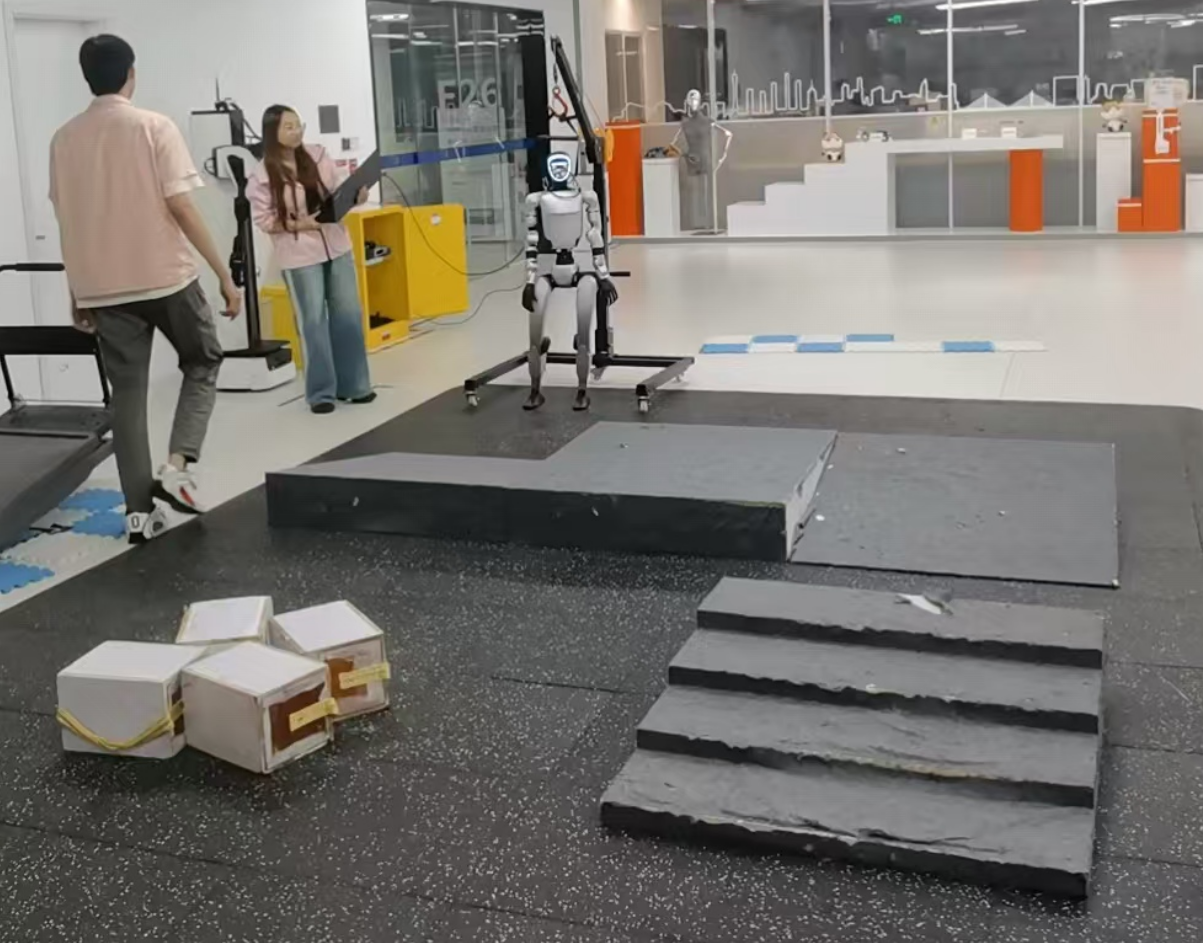
\includegraphics[width=\textwidth]{figures/ch7_terrain_overview.png}
    \caption{Overview of the real-robot experiment terrain setup. The four terrain types are: (a)~stairs connected to a slope, (b)~a second slope from the opposite direction, (c)~randomly placed large rocks, and (d)~a raised platform.}
    \label{fig:terrain_overview}
\end{figure}

\begin{table}[t]
\centering
\caption{Specifications of the terrain modules used in the real-robot experiments.}
\label{tab:terrain_specs}
\footnotesize
\begin{tabular}{@{}p{2.5cm}p{2.5cm}p{7.5cm}@{}}
\toprule
\textbf{Terrain} & \textbf{Footprint} & \textbf{Key Parameters} \\
\midrule
Stairs           & 1\,m $\times$ 1\,m & Total height 20\,cm, 4 steps; each step: width 1\,m, depth 25\,cm, height 5\,cm \\
Slope ($\times$2) & 1\,m $\times$ 1\,m & Height 20\,cm, slope angle $\arctan(0.2) \approx 11.3^\circ$ \\
Raised platform  & 1\,m $\times$ 1\,m & Height 20\,cm \\
Random rocks ($\times$4) & Each 30\,cm $\times$ 22\,cm $\times$ 20\,cm & Randomly placed on flat ground \\
\bottomrule
\end{tabular}
\end{table}

The stair and slope modules are arranged in sequence (stairs $\to$ slope) to test the policy's ability to transition between terrain types. The two slope modules are placed in different orientations to test directional robustness. The raised platform is tested from both approach directions (ascending and descending). The four rock blocks are placed at arbitrary positions and orientations on flat ground to create an unstructured stepping challenge.

All terrain modules share a common height of 20\,cm, which is comparable to the robot's foot length and represents a significant obstacle relative to the robot's leg length. The stair steps (5\,cm each) are intentionally low to test whether the policy can choose efficient multi-step climbing strategies rather than stepping on each individual tread.

%% ============================================================
\section{Experiment Results}
\label{sec:real_results}
%% ============================================================

Each terrain scenario was tested 2--3 times. The initial attempts had lower success rates due to infrastructure issues rather than policy failures: (1)~the Ethernet cable connector loosening during motion, causing communication loss; (2)~the laptop entering power-saving mode during long test sessions, reducing inference speed below the 50\,Hz requirement; and (3)~overly aggressive velocity commands sent via the wireless controller (maximum speed setting), causing excessively large motion amplitudes. Once these infrastructure and operational issues were resolved, the policy consistently produced stable locomotion across all terrain types at a walking speed of approximately 1\,m/s.

\subsection{Stairs Connected to Slope (First Run)}
\label{sec:stair_slope_first}

The first test scenario consists of the stair module connected to a slope module, requiring the robot to climb stairs, transition onto a slope, and descend from the slope to flat ground.

\paragraph{Stair climbing.}
Because each stair step is only 5\,cm high, the robot chooses to take two steps at a time, effectively treating the stairs as 10\,cm steps. This behavior emerges naturally from the policy's terrain-adaptive stepping strategy: the attention module perceives the low step height and determines that a single-step-per-stair gait would be unnecessarily cautious, while the energy penalty reward ($r_{\mathrm{energy}}$, weight $-5 \times 10^{-5}$, defined as the squared sum of torque $\times$ velocity normalized by stiffness) further discourages over-cautious stepping.

\paragraph{Attention-driven step placement at stair end.}
As the robot approaches the top of the stairs, the attention module detects the height difference at the stair-slope boundary. Rather than stepping onto the slope directly from the second-to-last step, the robot places its final step on the last stair tread, ensuring a stable foothold before transitioning to the slope (Figure~\ref{fig:stair_attention_last_step}). This behavior demonstrates that the attention module is not merely reacting to the current depth image but is integrating terrain context to plan the next foothold.

\begin{figure}[t]
    \centering
    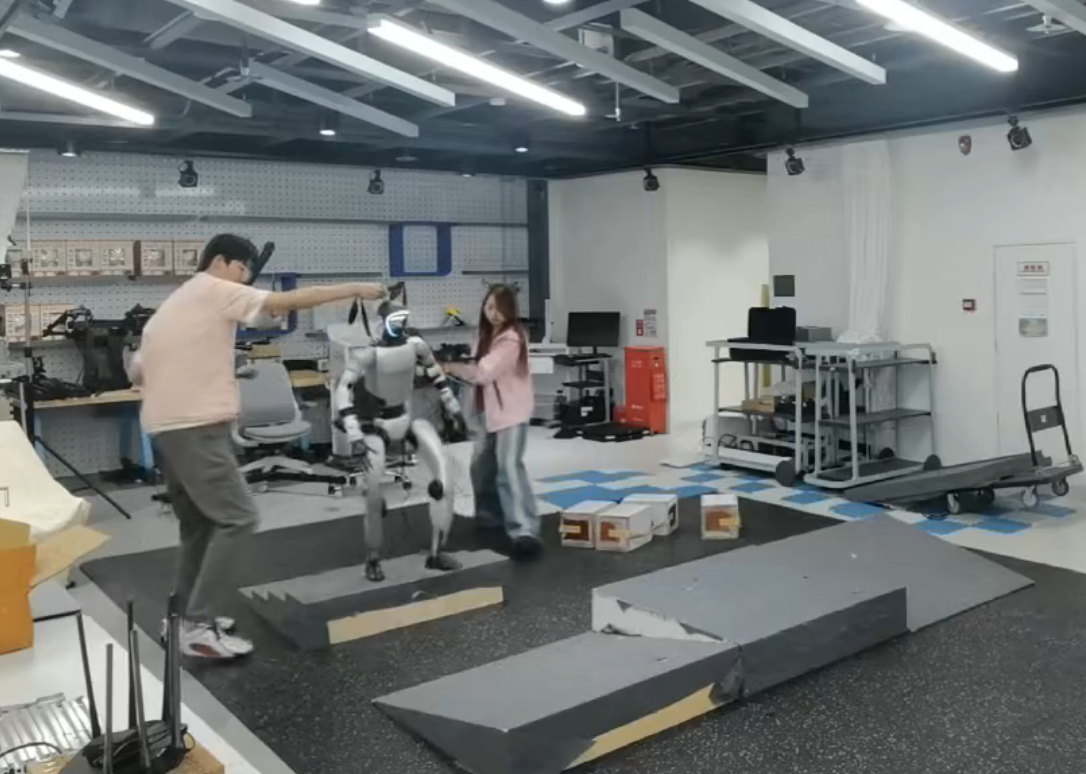
\includegraphics[width=0.9\textwidth]{figures/ch7_stair_attention_last_step.png}
    \caption{The robot climbing stairs connected to a slope. Through the attention mechanism, the robot detects the height difference at the stair end and chooses to place its final step on the last stair tread rather than stepping directly onto the slope, ensuring a stable foothold before the terrain transition.}
    \label{fig:stair_attention_last_step}
\end{figure}

\paragraph{Slope ascent.}
Upon reaching the slope, the depth camera provides visual input indicating the upward incline ahead. The robot responds by lifting its swing foot higher and shifting its center of gravity toward the mid-rear of the support polygon. Placing the center of gravity too far forward would result in insufficient shock absorption at foot landing, causing impact instability. The learned policy naturally adopts this conservative posture, which is consistent with the behavior observed in simulation on pyramid slope terrains (Chapter~\ref{chap:experimental_results}).

\paragraph{Slope descent with attention to edge.}
At the top of the slope, the attention module focuses on the sharp edge where the slope meets the flat ground. To avoid tripping on this edge, the robot adopts a conservative high-step gait for the final step off the slope, lifting the swing foot well above the edge before landing on flat ground (Figure~\ref{fig:slope_attention_edge}). This is another instance where the attention module identifies a specific geometric feature (the slope edge) and the policy adjusts its gait accordingly.

\begin{figure}[t]
    \centering
    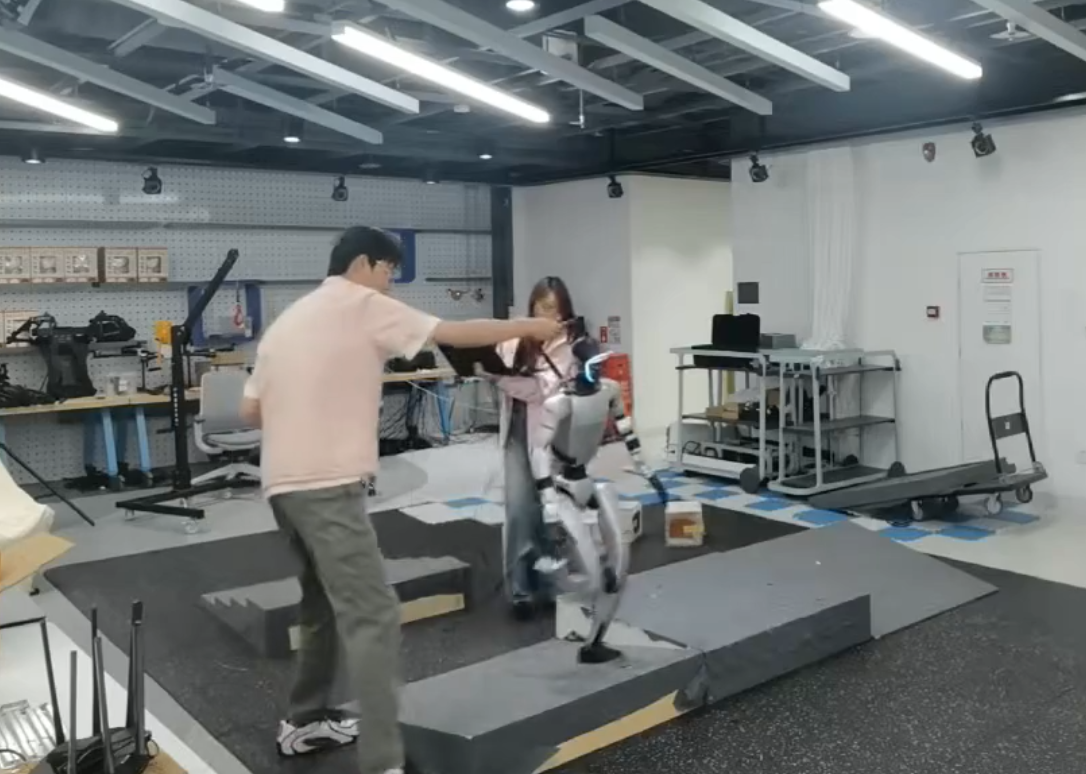
\includegraphics[width=0.9\textwidth]{figures/ch7_slope_attention_edge.png}
    \caption{The robot descending from the slope. The attention module focuses on the sharp edge at the slope top, and the robot adopts a conservative high-step gait to avoid tripping on the edge.}
    \label{fig:slope_attention_edge}
\end{figure}

\subsection{Slope from Opposite Direction}
\label{sec:slope_opposite}

After completing the stair-slope sequence, the robot approaches the second slope module from the opposite direction. The policy produces the same adaptive behaviors---higher foot lift on the slope, rear-shifted center of gravity, and cautious edge descent---demonstrating that the terrain-adaptive strategy is direction-invariant and robust to approach angle.

\subsection{Random Large Rocks}
\label{sec:random_rocks}

The most challenging scenario involves four large rock blocks (each 30\,cm $\times$ 22\,cm $\times$ 20\,cm) placed at arbitrary positions and orientations on flat ground. This terrain tests the combined effect of the attention and memory modules, as the robot must identify stable footholds among the rocks and retain terrain context when visual information becomes occluded.

\paragraph{Step 1: Attention identifies a flat foothold between rocks.}
The attention module identifies a patch of flat ground between two rocks that can serve as a stable foothold. The robot shifts its center of gravity toward this flat region and steps onto it, avoiding the surrounding rocks (Figure~\ref{fig:rocks_attention_memory}, top).

\paragraph{Step 2: Memory preserves terrain context under occlusion.}
After stepping onto the flat ground between the rocks, the depth camera's field of view no longer covers the area directly beneath the robot's feet---the rocks occlude the downward view. However, the memory module retains the information that there are rocks near the feet, and the robot lifts its swing foot high to avoid tripping on the rocks at foot level. This is a clear demonstration of the memory module's value: without memory, the robot would have no knowledge of the rocks beneath it once they leave the camera's field of view, and would likely trip. With memory, the robot proactively lifts its foot and steps securely onto the surface of a rock (Figure~\ref{fig:rocks_attention_memory}, bottom). The synergy between attention and memory is critical here: attention first identifies the flat ground as a stepping target, and memory then preserves the context about nearby rocks even after they leave the camera's view.

\begin{figure}[t]
    \centering
    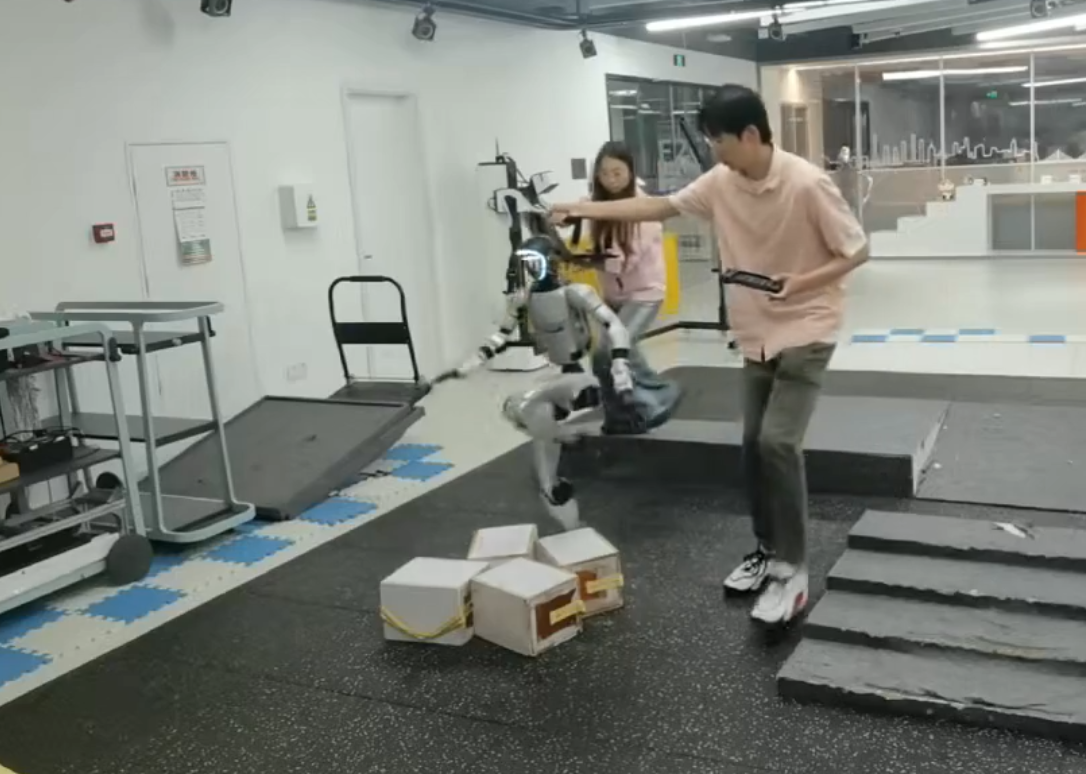
\includegraphics[width=0.9\textwidth]{figures/ch7_rocks_attention_memory.png}
    \caption{The robot navigating randomly placed large rocks. \textbf{Top:} The attention module identifies a flat patch of ground between the rocks and the robot steps onto it. \textbf{Bottom:} After the depth camera can no longer see the area near the feet (rocks occlude the downward view), the memory module retains the terrain context and the robot lifts its swing foot high to avoid tripping, stepping securely onto the rock surface.}
    \label{fig:rocks_attention_memory}
\end{figure}

\paragraph{Step 3: Attention selects the next rock foothold.}
From the top of the first rock, the attention module identifies the next rock's surface as a viable foothold. The robot steps across and lands precisely on the target rock (Figure~\ref{fig:rocks_attention_next_rock}).

\begin{figure}[t]
    \centering
    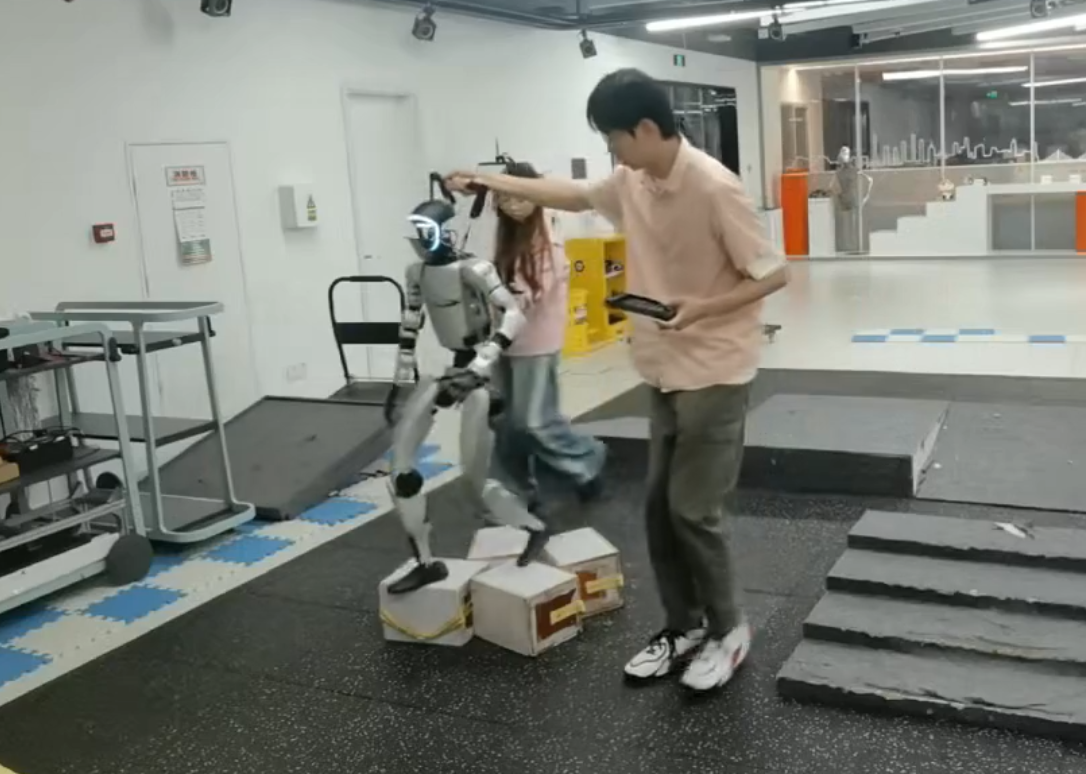
\includegraphics[width=0.9\textwidth]{figures/ch7_rocks_attention_next_rock.png}
    \caption{The robot stepping from one rock to the next. The attention module identifies the next rock's surface as a viable foothold, and the robot lands precisely on the target.}
    \label{fig:rocks_attention_next_rock}
\end{figure}

\paragraph{Step 4: Final step to flat ground.}
After traversing the rocks, the robot steps naturally onto the flat ground between the rocks and lands smoothly (Figure~\ref{fig:rocks_flat_ground}).

\begin{figure}[t]
    \centering
    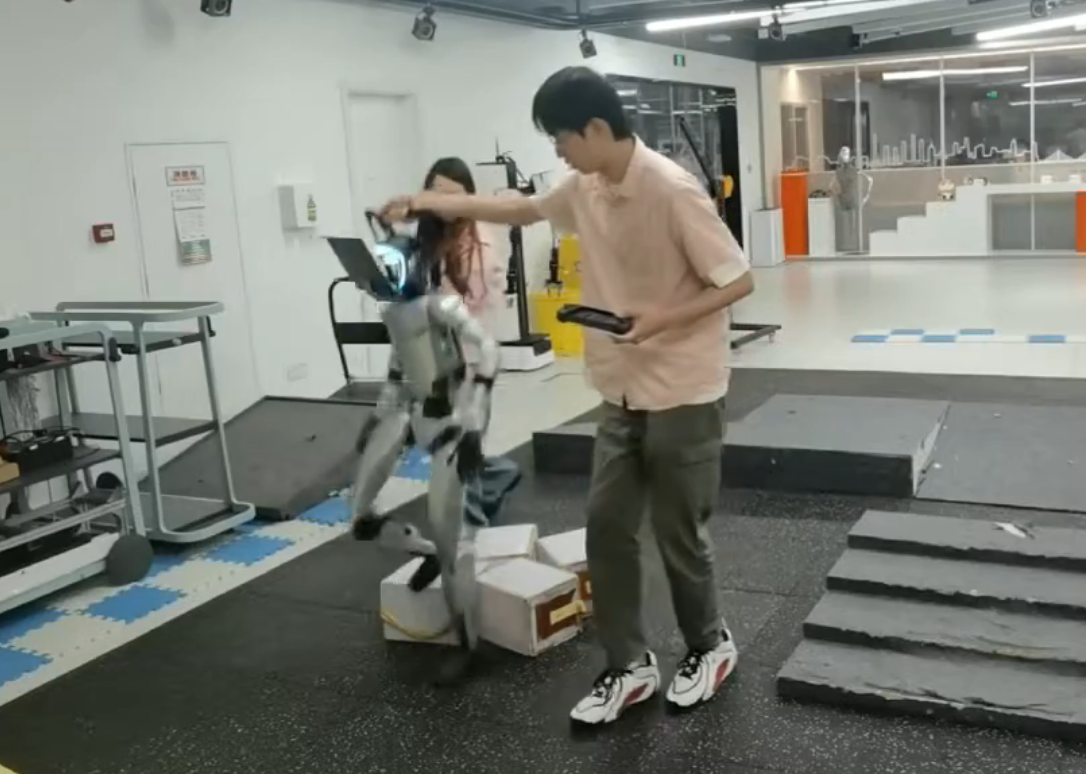
\includegraphics[width=0.9\textwidth]{figures/ch7_rocks_flat_ground.png}
    \caption{The robot's final step from the rocks onto flat ground, landing smoothly.}
    \label{fig:rocks_flat_ground}
\end{figure}

\subsection{Raised Platform}
\label{sec:raised_platform}

The robot is tested on the raised platform (1\,m $\times$ 1\,m, height 20\,cm) from two approach directions: ascending onto the platform and descending from the platform. In both cases, the robot produces natural walking motion without any issues, stepping onto and off the platform with appropriate foot height and body posture.

\subsection{Stairs Connected to Slope (Second Run --- Robustness Verification)}
\label{sec:stair_slope_second}

The stair-slope scenario is repeated to verify the robustness of the policy. In this second run, the robot exhibits a slightly different but equally valid strategy:

\paragraph{Alternative stair strategy.}
Unlike the first run where the robot stepped onto the last stair tread, in this run the robot does not step onto the last step. Instead, it lifts its swing foot over the highest remaining step and lands directly on flat ground beyond the stairs (Figure~\ref{fig:stair_step_over}). This demonstrates that the policy does not follow a fixed behavioral script but makes context-dependent decisions: the attention module perceives the terrain layout, the memory module retains the stair context, and the temporal-subsampled depth image stack provides a longer temporal horizon of depth information. Combined with the energy penalty reward that discourages unnecessary steps, the policy chooses the most efficient action---stepping over the last stair rather than stepping onto it.

\begin{figure}[t]
    \centering
    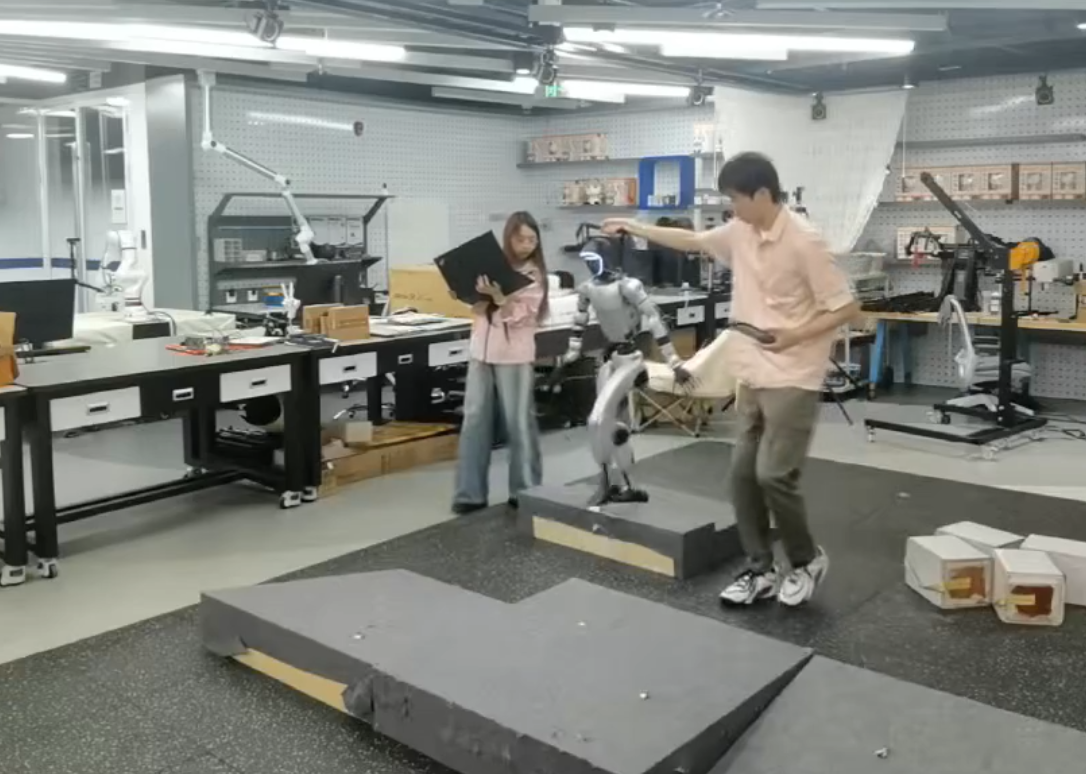
\includegraphics[width=0.9\textwidth]{figures/ch7_stair_step_over.png}
    \caption{The second run on the stair-slope terrain. Unlike the first run, the robot does not step onto the last stair tread but instead lifts its swing foot over the highest step and lands directly on flat ground, demonstrating energy-efficient and context-dependent decision making.}
    \label{fig:stair_step_over}
\end{figure}

\paragraph{Natural slope landing.}
At the end of the slope, the robot performs a small two-foot hop to transition from the slope to flat ground. This is a natural and energy-efficient motion that emerges from the AMP-trained gait style, rather than a cautious step-down (Figure~\ref{fig:slope_hop_landing}).

\begin{figure}[t]
    \centering
    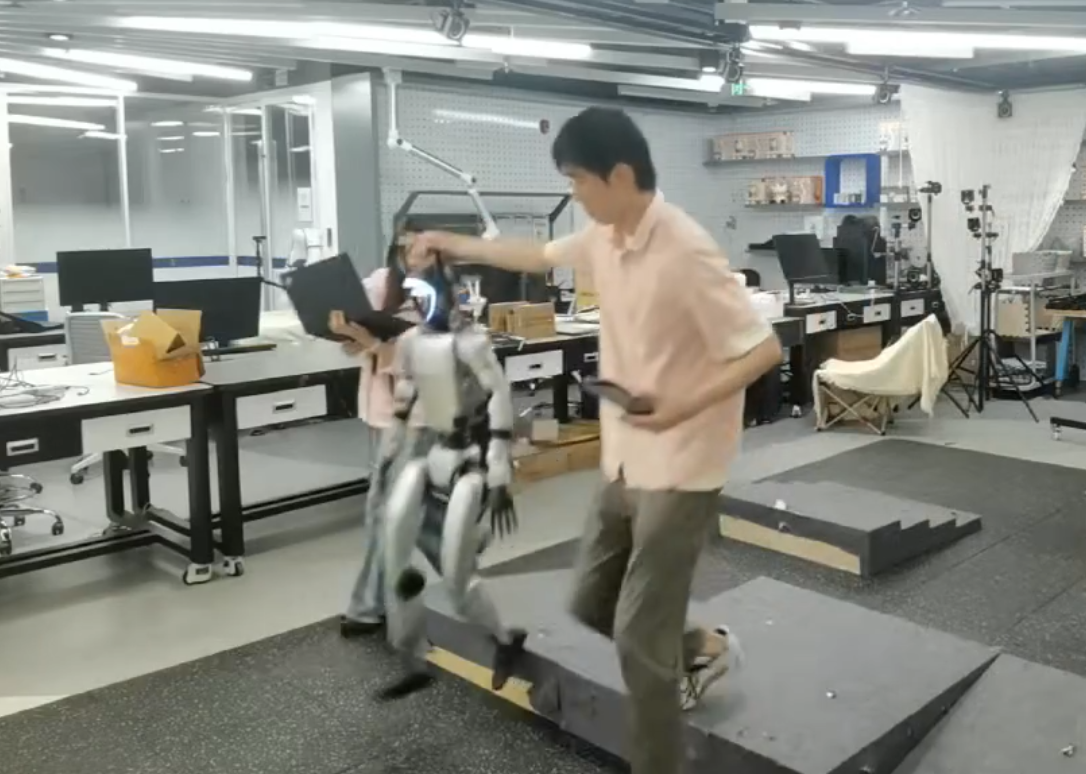
\includegraphics[width=0.9\textwidth]{figures/ch7_slope_hop_landing.png}
    \caption{The robot performing a small two-foot hop at the end of the slope to transition to flat ground, a natural and energy-efficient motion emerging from the AMP-trained gait style.}
    \label{fig:slope_hop_landing}
\end{figure}

%% ============================================================
\section{Discussion}
\label{sec:real_discussion}
%% ============================================================

\subsection{Natural Motion Style}
\label{sec:natural_motion}

A notable outcome of the real-robot experiments is the naturalness of the robot's motion. The walking gait, foot placement, and body posture adjustments all appear fluid and human-like. This is attributed to the AMP discriminator (Chapter~\ref{chap:proposed_method}), which provides a style reward that encourages the policy to imitate the reference motion data, combined with the MoE architecture that allows different experts to specialize in different terrain conditions. Without AMP, the robot's gait would be functional but robotic---achieving the task without the stylistic quality that makes the motion appear natural.

\subsection{Attention, Memory, and Temporal Depth Synergy}
\label{sec:attention_memory_synergy}

The rock terrain experiment provides the clearest evidence of the three perception components working together:

\begin{enumerate}
    \item \textbf{Attention} identifies the relevant terrain feature (flat ground between rocks, the next rock surface, the slope edge).
    \item \textbf{Memory} preserves terrain context when the depth camera can no longer see the area near the feet (rocks occluding the downward view).
    \item \textbf{Temporal depth stacking} (frame subsampling) extends the effective perception horizon, allowing the robot to retain depth information from several steps ago. The policy receives 8 depth frames subsampled from a 37-frame history at 5-frame intervals, providing an effective lookback of approximately 3.6\,s.
\end{enumerate}

Without any one of these components, the robot would likely fail on the rock terrain: without attention, it would not identify the correct foothold; without memory, it would lose track of rocks near its feet once they leave the camera's view; without temporal stacking, the depth perception horizon would be too short to inform multi-step planning.

The second stair-slope run further illustrates this synergy: the robot's decision to step over the last stair rather than onto it requires (1)~attention to perceive the terrain layout, (2)~memory to retain the stair context, and (3)~temporal depth stacking to provide a longer perception horizon. The energy penalty reward then biases the policy toward the more efficient option, but only because the perception modules provide sufficient information to the policy to determine that stepping over is safe.

\subsection{Energy-Efficient Decision Making}
\label{sec:energy_efficient}

The second run on the stair-slope terrain demonstrates that the policy makes energy-efficient decisions. By stepping over the last stair rather than stepping onto it, the robot avoids an unnecessary step. This behavior is shaped by the energy penalty reward during training ($r_{\mathrm{energy}}$, weight $-5 \times 10^{-5}$, computed as the squared sum of motor power $\tau \cdot \dot{q}$ normalized by stiffness) and enabled by the combined perception of attention, memory, and temporal depth stacking, which give the robot sufficient information to determine that stepping over is safe. Similarly, the two-foot hop at the end of the slope is a natural, energy-efficient transition that emerges from the AMP-trained gait style.

%% ============================================================
\section{Limitations}
\label{sec:real_limitations}
%% ============================================================

\begin{itemize}
    \item \textbf{Safety harness interference:} The safety harness attached to the robot's shoulders occasionally applied inadvertent tension to the robot, causing unnecessary balance corrections. This is visible in the supplementary video and slightly degrades the apparent motion quality. A fully autonomous deployment without the harness would be needed to evaluate the policy's true fall-recovery capability.

    \item \textbf{Communication reliability:} Ethernet cable disconnection was a recurring issue during testing, causing communication loss and robot falls. This is a hardware infrastructure problem rather than a policy limitation, but it highlights the importance of robust communication (or fully onboard computing) for autonomous operation.

    \item \textbf{External computing dependency:} The current deployment relies on an external laptop for policy inference, which limits the robot's autonomy and introduces a communication dependency. Future work should transition to onboard computing (e.g., NVIDIA Jetson Orin NX) to enable fully autonomous operation.

    \item \textbf{Limited extreme terrain testing:} The experiments were conducted on terrain modules with a maximum height of 20\,cm. The policy's performance on more extreme terrain (higher steps, steeper slopes, larger gaps) remains to be evaluated.

    \item \textbf{Velocity command sensitivity:} When the operator sends overly aggressive velocity commands (maximum speed via the wireless controller), the resulting motion amplitudes can exceed the policy's stable operating regime. Tuning a better command limiter would enhance robustness.
\end{itemize}

\end{document}